% !TeX program = latexmk
% Generated from the reference PDF text layer; full PDF pages are not embedded.
\PassOptionsToPackage{bookmarks=false}{hyperref}
\documentclass[withoutpreface,bwprint]{cumcmthesis}
\usepackage{url}
\usepackage{subcaption}
\usepackage{graphicx}
\usepackage{svg}
\usepackage{fvextra}
\IfFontExistsTF{Noto Sans SC}
  {\newfontfamily\PDFTextFont{Noto Sans SC}}
  {\newfontfamily\PDFTextFont{FandolHei-Regular.otf}}
\setmonofont{Latin Modern Mono}
\setCJKmonofont{FandolFang-Regular.otf}
\newcommand{\CodeTextSetup}{\xeCJKsetup{CJKecglue={},CJKglue={}}}
\renewcommand{\theFancyVerbLine}{\normalfont\small\arabic{FancyVerbLine}}
\DefineVerbatimEnvironment{CodeText}{Verbatim}{fontsize=\small,numbers=left,numbersep=10pt,xleftmargin=0pt,breaklines=true,breakanywhere=false,breaksymbolleft={},breaksymbolright={},formatcom=\CodeTextSetup,listparameters={\setlength{\topsep}{0pt}\setlength{\partopsep}{0pt}\setlength{\parsep}{0pt}}}
\setlength{\parskip}{0pt}
\sloppy

\makeatletter
\renewenvironment{abstract}{%
\if@twocolumn
    \section*{\abstractname}%
  \else
   \begin{center}%
  {\zihao{4}\bfseries \abstractname\vspace{-.5em}\vspace{\z@}}%
   \end{center}%
   \quotation
  \fi}
  {\if@twocolumn\else\endquotation\clearpage\fi}
\makeatother

\title{基于动态搜索的“板凳龙”运动状态及路线研究}
\tihao{A}
\baominghao{}
\schoolname{}
\membera{}
\memberb{}
\memberc{}
\supervisor{}
\yearinput{2024}
\monthinput{9}
\dayinput{8}

\begin{document}
\maketitle

\begin{abstract}
板凳龙作为浙闽地区的一种传统民俗活动，以其高观赏性和舞龙队的协调配合著称。本文针对板凳龙表演的三个阶段——盘入、调头和盘出，通过分析舞龙队的行进路线及各节板凳之间的几何关系，建立了运动模型和行进路线优化模型。采用多种优化方法，对舞龙队在不同条件下的运动状态以及行进路线进行研究。

\textbf{针对问题一：}构建盘入运动模型。首先，根据盘入路线为等距螺线的特征，建立\textbf{极坐标系}。针对龙头位置，建立有关极角的微分方程，利用微积分及\textbf{二分法}求解龙头前把手的极坐标，继而利用\textbf{余弦定理}，\textbf{递推求解}相邻板凳的位置关系，获得各把手的位置函数。通过对位置函数求导，得到相应的速度函数。最终，将极坐标转换为直角坐标，求得各把手在各时刻的位置和速度，结果详见\textbf{表2，表3和result1.xlsx}。

\textbf{针对问题二：}构建碰撞检测模型。首先，证明最易发生碰撞的区间为最内圈与其外侧一圈的板凳，缩小检测范围。随后，确定\textbf{碰撞条件}为：内圈板凳顶点与外圈板凳把手连线的距离小于板凳宽度的一半（0.15m），并通过几何关系算出\textbf{距离函数}，判断该函数的最小值是否小于0.15m 以确定碰撞是否发生。最后，采用\textbf{动态搜索策略}，先用变步长搜索确定时间范围，再进行二分搜索，确定首次碰撞的准确时间。我们得到停止盘入时间为\textbf{412.473838s}，此时各把手的位置和速度详见\textbf{表4和result2.xlsx}。

\textbf{针对问题三：}构建最短螺距的\textbf{单目标优化}模型。其中目标函数和决策变量为螺距大小。在约束条件方面，基于板凳的几何参数和问题二中的参数限定螺距范围，基于盘入运动模型确定龙头前把手进入调头空间的时间，并利用碰撞检测模型判断进入调头空间前是否发生碰撞，建立相应约束。在优化求解过程中，对比后选用\textbf{粒子群算法}求解板间最小距离，并结合\textbf{变步长搜索}求得最短螺距为\textbf{0.450337m}。

\textbf{针对问题四：}基于问题一的模型，构建调头运动模型。首先证明在给定条件下，调头曲线长度为常数，\textbf{无法进一步减小}。随后，将调头路线划分为四个部分，通过几何关系求解出各部分的曲线方程。沿用问题一的推导方法，首先求解龙头前把手位置函数，再通过递推关系和求导计算其余把手的位置函数和速度函数。我们对调头空间附近的递推进行了详细的\textbf{分类讨论}，并给出了相应的\textbf{递推方程}。最终，将极坐标转换为直角坐标，求得各板凳把手在各时刻的位置和速度，详见\textbf{表5，表6和result4.xlsx}。

\textbf{针对问题五：}在调头运动模型的基础上，构建各把手最大速度的优化模型。首先，通过\textbf{比例转换}，将目标转化为在龙头速度仍为1m/s 的条件下，求解各把手在所有时刻的最大速度。随后，基于问题四的速度规律及物理规律确定最大速度出现的大致时间范围，接着通过大步长搜索确定了最大速度出现的区间为[\textbf{14s},\textbf{15s}]。由于函数在该区间内\textbf{呈单峰性}，应用\textbf{三分搜索算法}进一步精确定位最大速度。最后，通过比例关系还原龙头的最大速度，得到龙头最大速度约为\textbf{1.246266m/s}。

\keywords{板凳龙\quad 等距螺线\quad 动态搜索\quad 粒子群算法\quad 单目标优化}
\end{abstract}

\section{问题重述}
\subsection{问题背景}
中药材在加工后需要及时脱除水分，以提高储藏稳定性并保持成品品质。热风方式利用空气与药材之间的温差和湿度差完成热量、水分交换，药材内部经历由外向内的升温过程，同时水分由内部逐步迁移至表面并逸出。整个过程可分为升温过渡阶段和后续恒温脱水阶段，两个阶段的传热传质特征并不完全相同。

烘房温度、湿度及物性参数的组合会直接影响干燥速率、能耗和最终品质，单纯依靠反复试验难以系统考察这些因素的作用。为此，本文从连续介质传热与传质角度描述药材内部状态的时空变化，并结合数值计算比较不同干燥阶段及尺寸变化对结果的影响，为干燥时间判定和工艺参数分析提供依据。

\subsection{问题提出}
如图2所示，研究对象取为一段长度$25\,\mathrm{cm}$、半径$2\,\mathrm{cm}$的圆柱状药材。计算开始时，药材内部温度和干基含水率分别为$28\,{}^{\circ}\mathrm{C}$和$2.55\,\mathrm{kg/kg}$。附件同时提供烘房环境状态的时间序列以及干燥过程中药材半径的变化信息。本文据此建立模型并完成下列任务。

\begin{figure}[H]
\centering
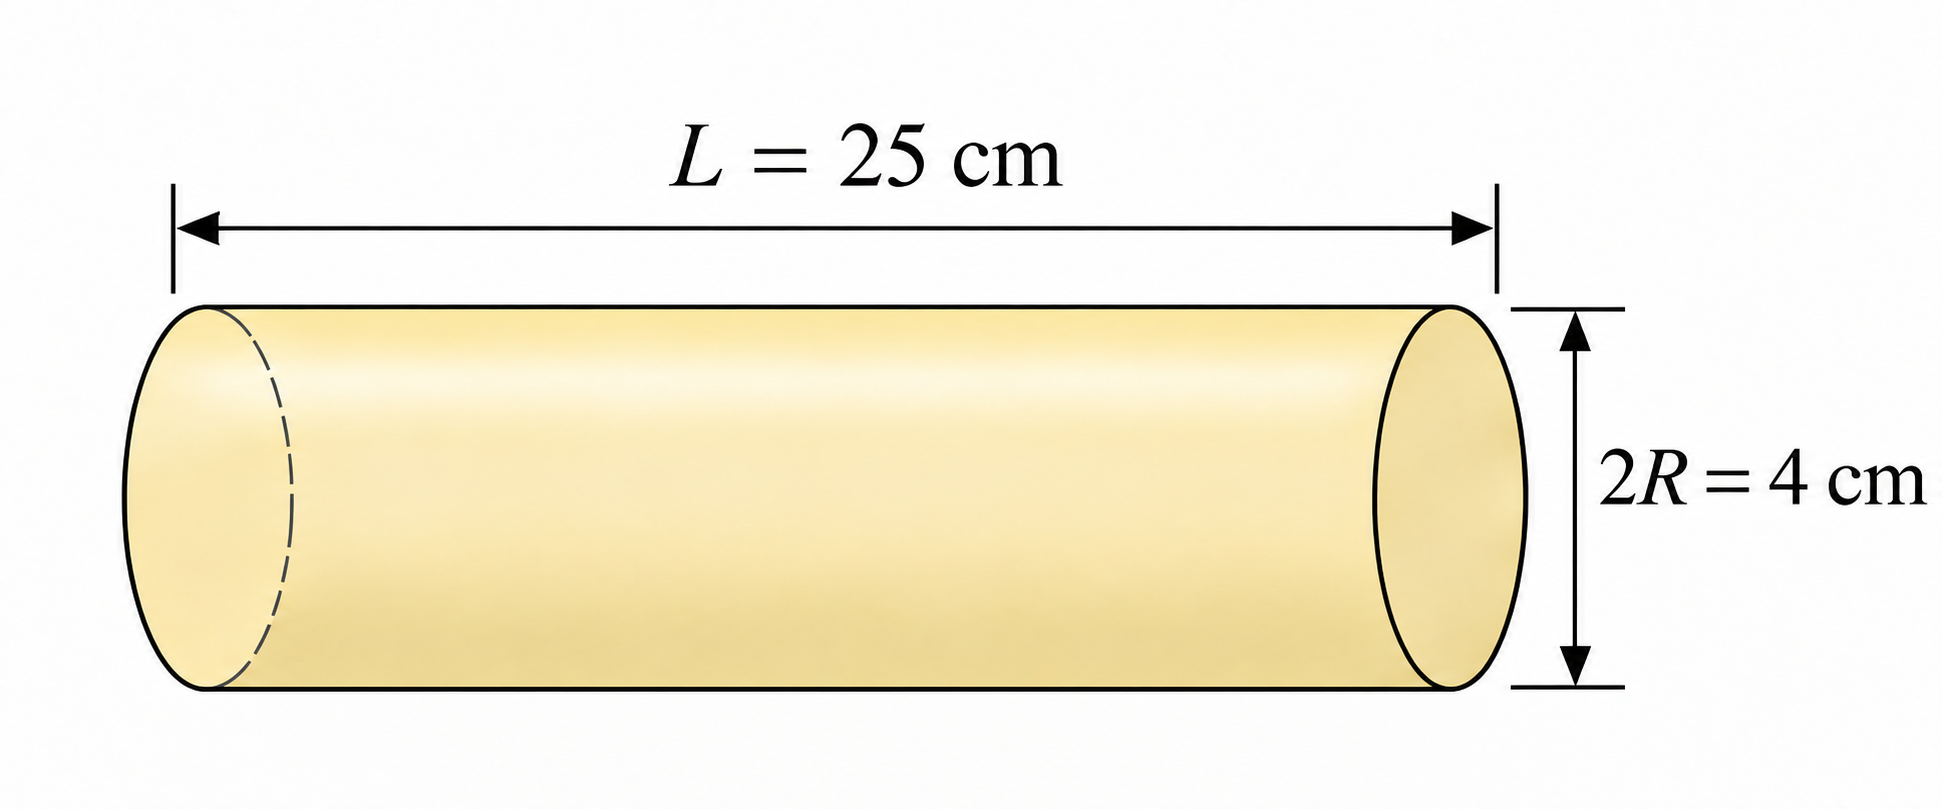
\includegraphics[width=0.8\textwidth]{figures/圆柱.png}
\caption{药材几何外形示意图}
\end{figure}

\textbf{问题一：}首先研究干燥开始后的$1800\,\mathrm{s}$预热阶段。利用附件1的烘房环境数据和附录2给出的物性参数，求解药材内部温度和含水率随时间及径向位置的分布。

\textbf{问题二：}在完整干燥过程的计算中，采用附录3的统一经验关系描述物性参数随状态的变化，建立温度场与含水率场的耦合模型。

\textbf{问题三：}在半径保持不变的条件下，以药材各处含水率均低于$0.15\,\mathrm{kg/kg}$作为干燥完成判据，确定达到该判据所需的时间。

\textbf{问题四：}进一步考虑药材失水后半径随时间收缩的情况，利用附件2的半径数据和附录4的经验关系修正传质计算域，重新确定达到$0.15\,\mathrm{kg/kg}$判据的干燥时长。

\section{问题分析}
\subsection{问题一}
问题一要求刻画预热平衡阶段药材内部温度和水分浓度随时间及径向位置的变化规律。由于药材可近似为均质、各向同性的细长圆柱体，其长度与半径之比为$12.5$，两个端面的总面积仅为侧面积的$8\%$，因此可忽略轴向梯度和端部效应，将问题简化为固定半径圆柱内的一维轴对称非稳态传热与传质问题(如图3)，从而将温度场与水分场作为两个相互并行的偏微分方程分别求解。对于温度场，根据Fourier导热定律和能量守恒建立圆柱坐标下的一维径向非稳态热传导方程，在圆柱中心设置对称边界，在药材表面设置Newton对流换热边界。对于水分场，根据Fick扩散定律和质量守恒建立径向扩散方程。为求解上述温度场和水分场的偏微分方程，本文采用径向有限体积法进行空间离散，并采用后向Euler全隐式格式进行时间离散与推进。

\begin{figure}[H]
\centering
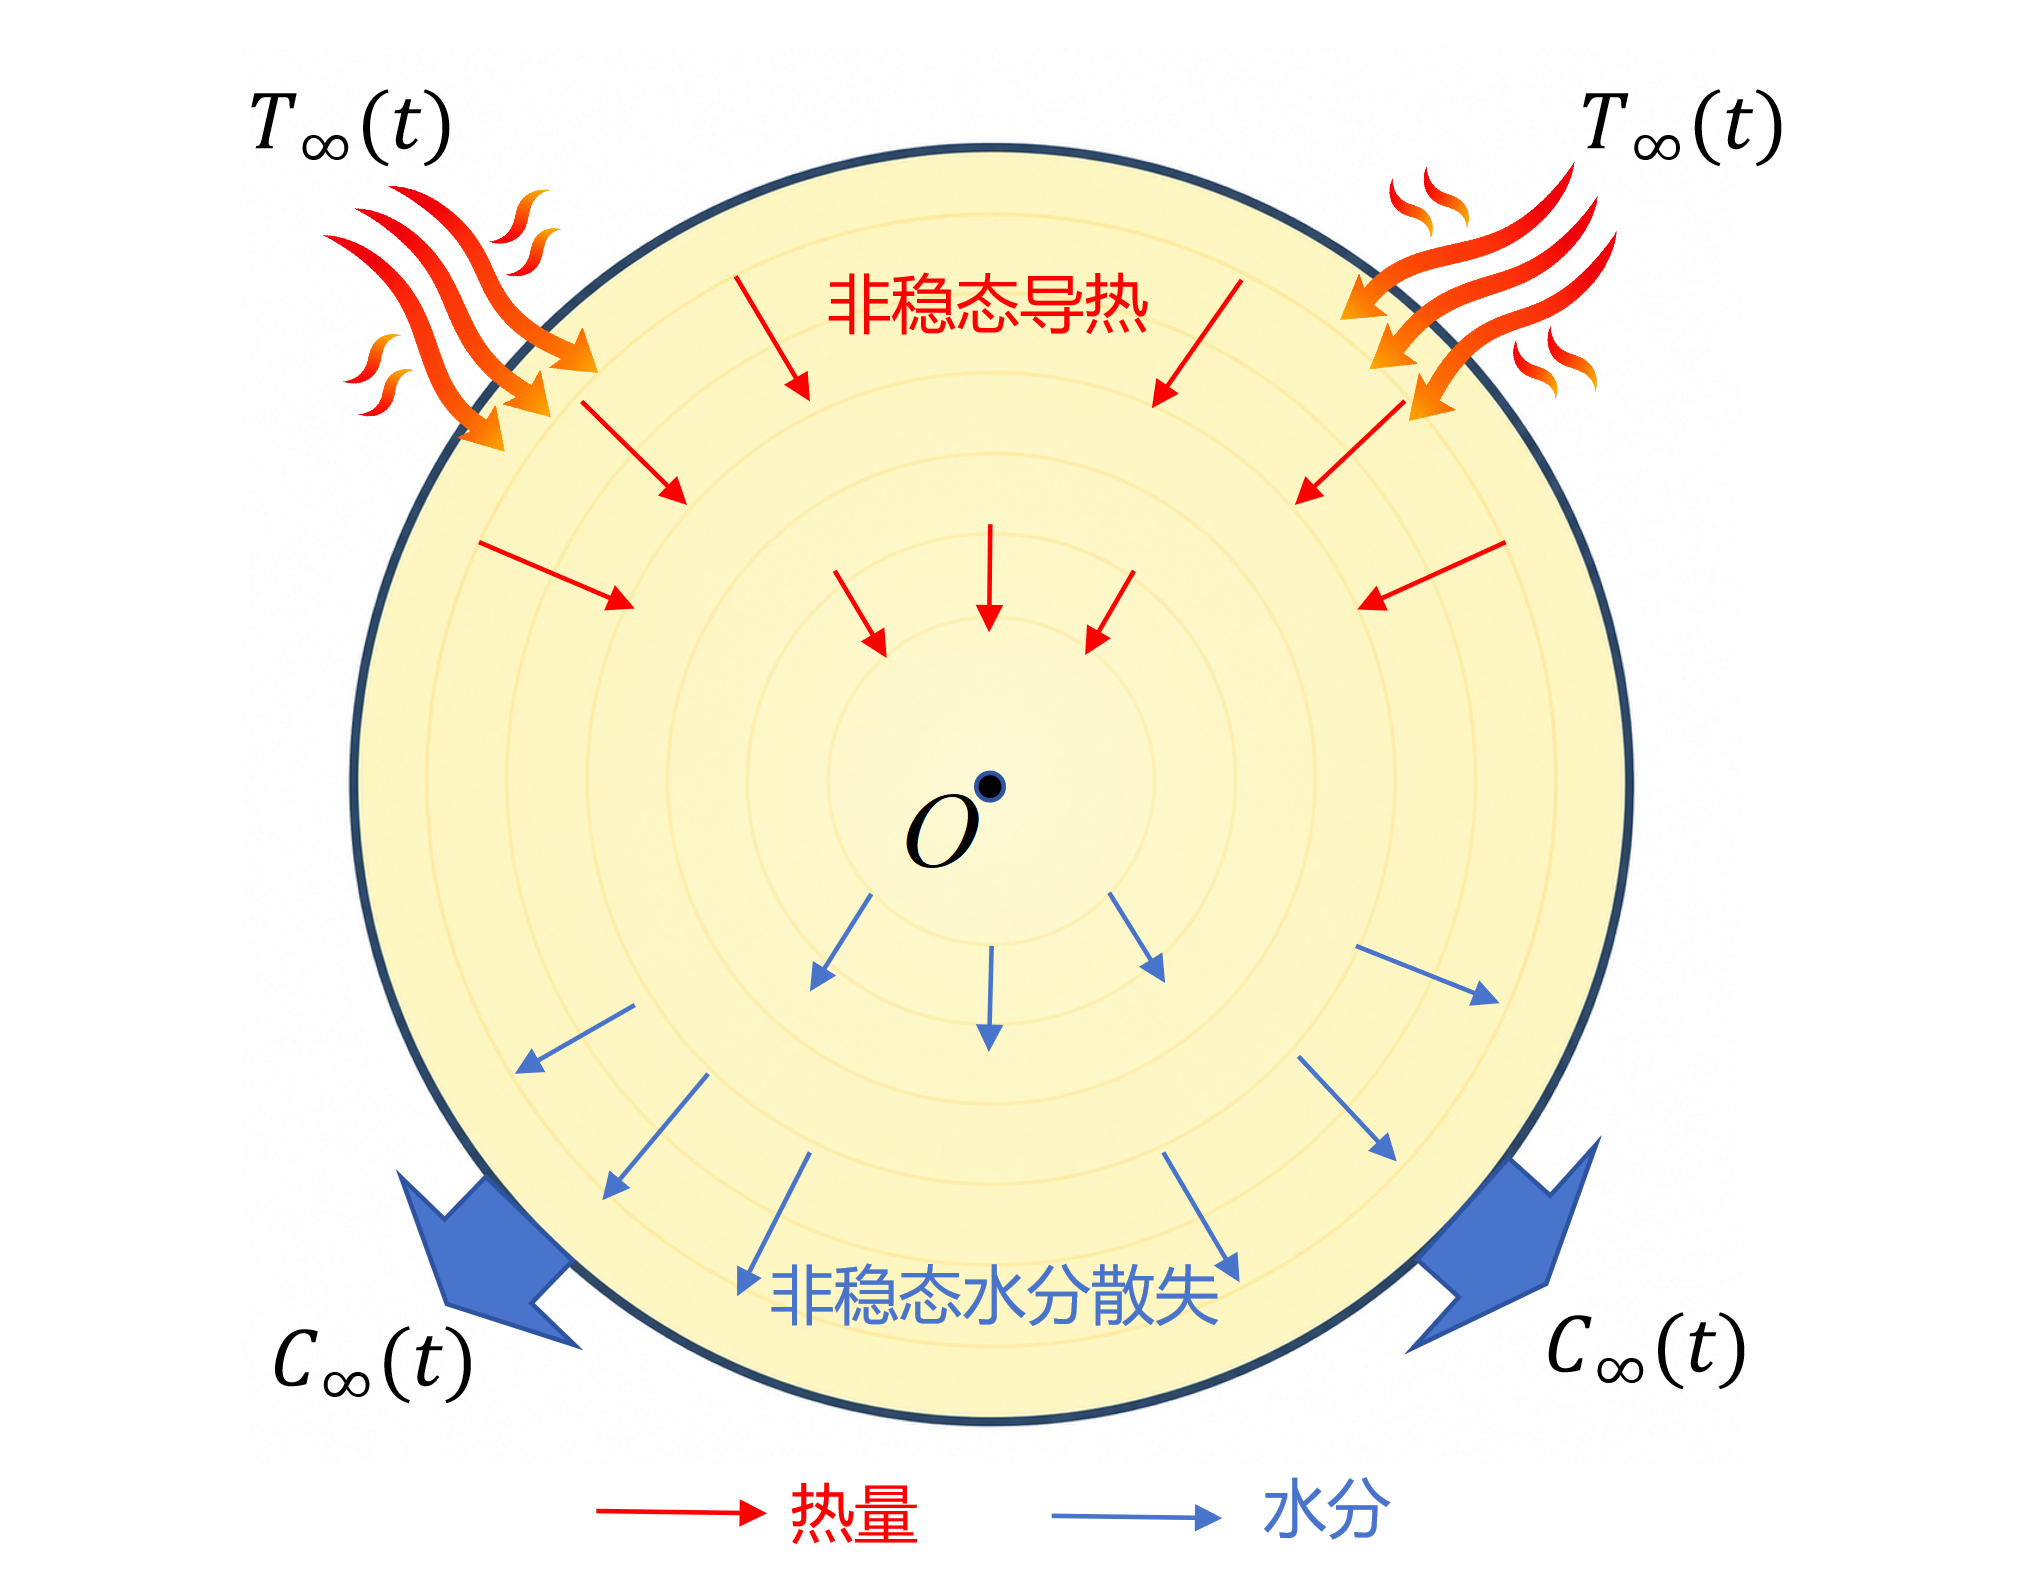
\includegraphics[width=0.8\textwidth]{figures/问题重述热量水分.png}
\caption{药材径向传热传质示意图}
\end{figure}


\subsection{问题二}
问题二沿用问题一建立的一维径向“传热-传质”模型，但进一步考虑药材物性参数随温度和含水率变化的影响。如图\ref{fig:q2-flowchart}所示，密度、比热容和导热系数由含水率决定，水分扩散系数则同时受含水率和绝对温度影响，因此温度场与水分场通过变物性参数形成间接双向耦合。模型从烘干初始状态开始计算，环境温度和水分浓度边界沿用分段线性插值结果。求解时采用与问题一一致的径向有限体积法和后向 Euler 全隐式格式，在每个时间层内交替更新变物性参数并采用 Picard 迭代求解，直至温度场和水分场同时收敛，进而获得前$3\,\mathrm{h}$内各时刻、各径向位置处的温度和水分浓度。

\begin{figure}[H]
\centering
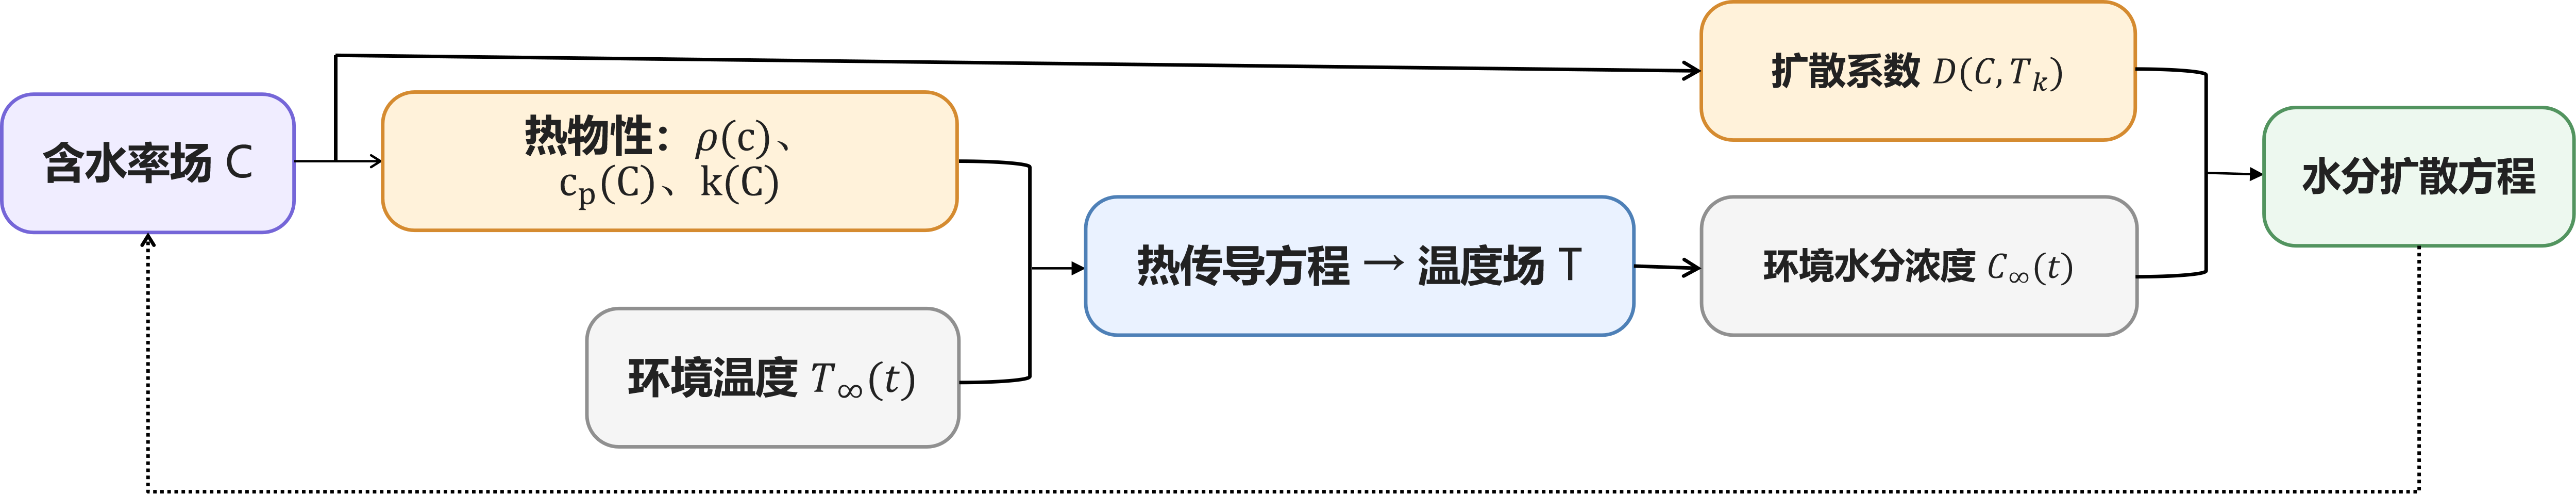
\includegraphics[width=0.95\textwidth]{figures/问题二流程图.png}
\caption{问题二热湿耦合计算流程图}
\label{fig:q2-flowchart}
\end{figure}

\subsection{问题三}
问题三要求确定药材各处干基含水率均低于$0.15\,\mathrm{kg/kg}$的时刻。本文继承问题二的固定半径变物性模型，先对附件1测量区间以外的环境边界作连续延拓，再以全域最大含水率构造终止事件。主计算采用表面加密的有限体积网格和变步长 BDF2 格式，通过独立的空间、时间加密估计数值不确定性；随后利用采用不同空间离散和时间推进的 Chebyshev 谱元--Radau 方法复算同一径向模型，检验临界时刻是否依赖单一数值实现。

\subsection{问题四}
问题四将固定半径模型推广到实测半径驱动的收缩区域。首先依据干基含水率定义与干质量守恒，检验附录4密度关系和附件2几何数据的相容性，说明即使放弃均匀仿射收缩，精确局部湿体积密度、实测半径、干质量守恒与长度不增加也不能全部满足。随后明确主模型的闭合选择：保留实测半径，采用固定长度和径向仿射运动，将题给密度关系用于有效显热储存，并在材料坐标中求解移动边界热湿耦合方程。最后通过真实密度下的长度反演和自由半径预测两组守恒对照，讨论烘干时长对模型结构的依赖，区分数值收敛与物理有效性。

\subsection{问题五}
问题五的目的是建立一个优化模型，求解最大速度。首先需要在问题四的基础上，计算全过程中各把手的最大速度。其次需要对问题四的结果进行分析，结合物理规律，缩小搜索范围。最后依据速度最大值函数的特征，采用适当的算法求解最大速度。

\section{建模假设}
\begin{enumerate}[label=\arabic*.,leftmargin=2em,itemsep=0pt,topsep=0pt]
  \item \textbf{连续、均质、各向同性：}在宏观尺度上，将药材等效为连续、均质且各向同性的多孔介质，忽略纹理方向、孔隙结构及分层物性等信息以及各向异性的导热和扩散参数。
  \item \textbf{一维径向近似：}药材长度远大于半径，端面相对于侧面的面积较小，因此忽略周向变化和主体区域的轴向端部效应，只考虑径向传热与传质。
  \item \textbf{忽略蒸发散热：}水分蒸发会带走汽化潜热，但题目未给出汽化潜热、蒸发速率及相变动力学参数，因此温度方程中不显式加入蒸发吸热项；由此产生的影响作为模型误差处理。同时忽略体热源、化学反应热、辐射换热和热扩散引起的直接水分通量。
  \item \textbf{局部宏观平均：}将温度场 $T(r,t)$ 和干基含水率场 $C(r,t)$ 视为连续场变量，微观孔隙内的气液界面不单独解析，其影响等效包含在 $k$ 和 $D$ 中。

\end{enumerate}


\section{符号说明}
{\centering\textbf{表1\quad 符号说明}\par}
\begin{table}[H]
\centering
\renewcommand{\arraystretch}{1.12}
\begin{tabularx}{0.96\textwidth}{>{\centering\arraybackslash}p{0.18\textwidth}X>{\centering\arraybackslash}p{0.24\textwidth}}
\toprule
符号 & 含义 & SI单位 \\
\midrule
$L$ & 药材长度 & $\mathrm{m}$ \\
$R_0$ & 药材初始半径 & $\mathrm{m}$ \\
$r$ & 到圆柱中心轴的物理距离 & $\mathrm{m}$ \\
$R(t)$ & 当前药材半径；前三问为 $R_0$ & $\mathrm{m}$ \\
$t$ & 时间 & $\mathrm{s}$ \\
$T(r,t)$ & 药材温度 & $^\circ\mathrm{C}$ \\
$T_K(r,t)$ & 绝对温度，$T_K=T+273.15$ & $\mathrm{K}$ \\
$C(r,t)$ & 干基含水率，即水质量与绝干物质量之比 & $\mathrm{kg/kg}$ \\
$T_\infty(t)$ & 烘房环境温度 & $^\circ\mathrm{C}$ \\
$C_\infty(t)$ & 与表面传质模型匹配的环境等效含水率 & $\mathrm{kg/kg}$ \\
$\rho$ & 表观密度 & $\mathrm{kg/m^3}$ \\
$c_p$ & 比热容 & $\mathrm{J/(kg\cdot K)}$ \\
$k$ & 导热系数 & $\mathrm{W/(m\cdot K)}$ \\
$D$ & 有效水分扩散系数 & $\mathrm{m^2/s}$ \\
$h$ & 表面对流换热系数 & $\mathrm{W/(m^2\cdot K)}$ \\
$h_m$ & 表面对流传质系数 & $\mathrm{m/s}$ \\
$\xi$ & 第四问的无量纲材料坐标，$\xi=r/R(t)$ & $1$ \\
\bottomrule
\end{tabularx}
\end{table}

药材初始长度和半径分别为 $L=25\,\mathrm{cm}$、$R_0=2\,\mathrm{cm}$，初始状态为 $T(r,0)=28\,{}^\circ\mathrm{C}$、$C(r,0)=2.55\,\mathrm{kg/kg}$。
其中 $C$ 为干基含水率，数值 $2.55$ 表示每 $1\,\mathrm{kg}$ 绝干药材含 $2.55\,\mathrm{kg}$ 水。


\section{模型建立与求解}
\subsection{问题一模型的建立与求解}

\begin{figure}[H]
\centering
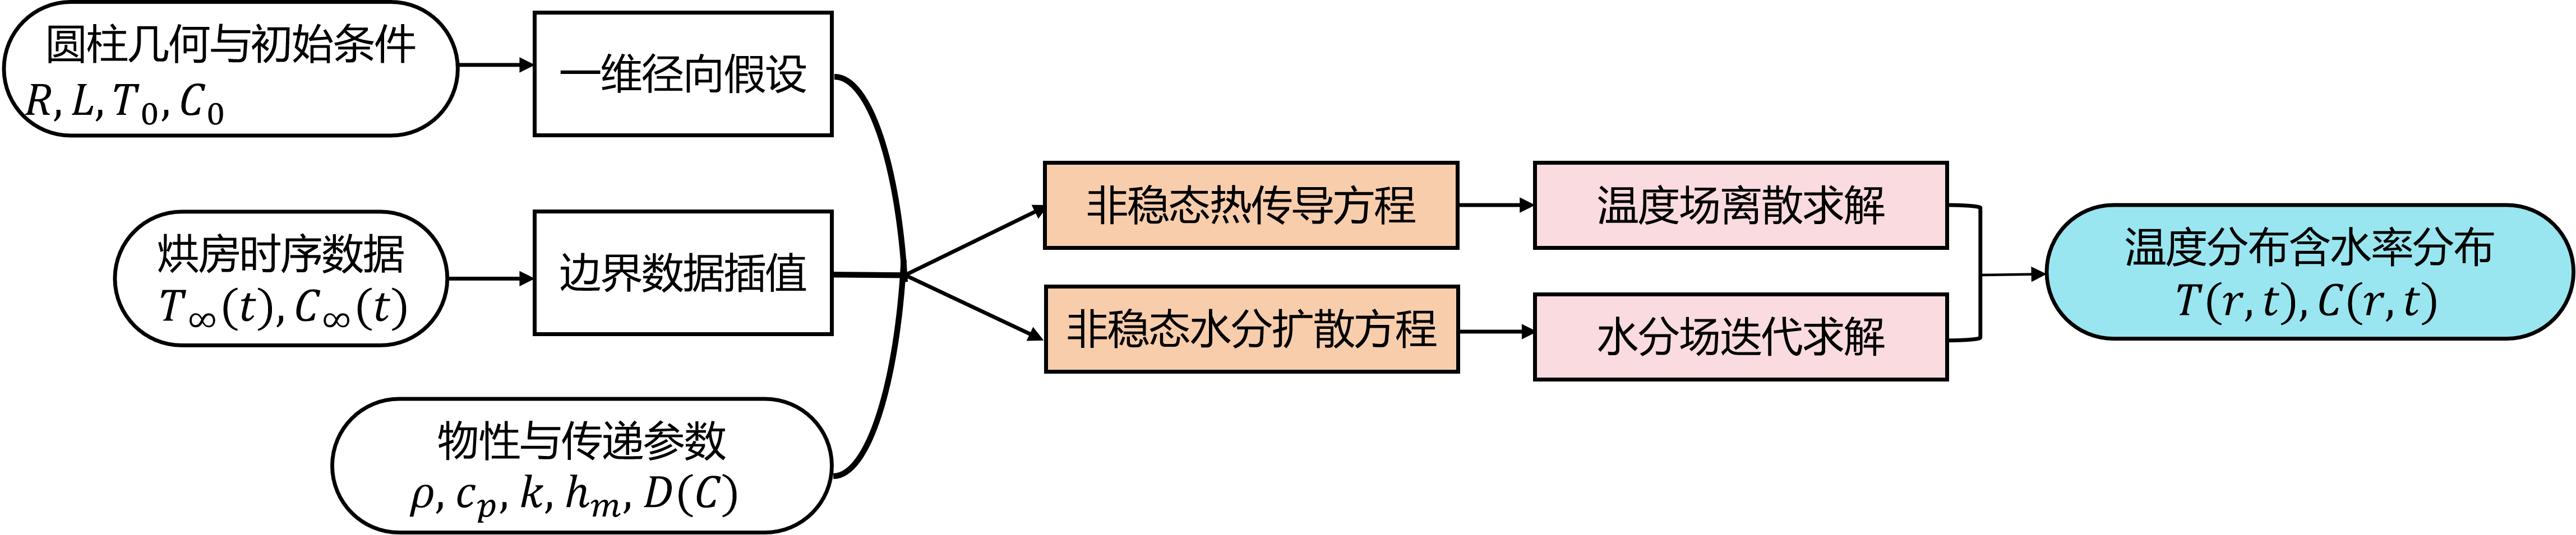
\includegraphics[width=0.9\textwidth]{figures/问题一流程图.png}
\caption{问题一流程图}
\end{figure}

\subsubsection{线性插值处理}
附件1给出的烘房温度和水分浓度为时间间隔$60\,\mathrm{s}$的离散采样序列，而数值离散的时间层间隔为$1\,\mathrm{s}$。为获得各计算时间层对应的边界状态，本文对该采样序列进行分段线性插值。设相邻采样时刻为$t_j$和$t_{j+1}$，则当$t\in[t_j,t_{j+1}]$时，有
\begin{equation}
\left\{
\begin{aligned}
T_\infty(t)&=T_{\infty,j}
+\frac{t-t_j}{t_{j+1}-t_j}
\left(T_{\infty,j+1}-T_{\infty,j}\right)\\
C_\infty(t)&=C_{\infty,j}
+\frac{t-t_j}{t_{j+1}-t_j}
\left(C_{\infty,j+1}-C_{\infty,j}\right)
\end{aligned}
\right.
\label{eq:environment-interpolation}
\end{equation}
该插值仅用于构造连续变化的边界条件，不改变附件1的原始采样数据。



\subsubsection{温度场模型}

为清晰表征药材内部传热、传质过程及其边界交换关系，图\ref{fig:q1-radial-process}示意了一维径向非稳态热传导与水分扩散过程。模型中，药材中心取轴对称条件作为内边界，药材表面与烘房环境之间分别以对流换热和对流传质进行热量与水分交换；后续温度场与水分场控制方程即基于此建立。

\begin{figure}[H]
\centering
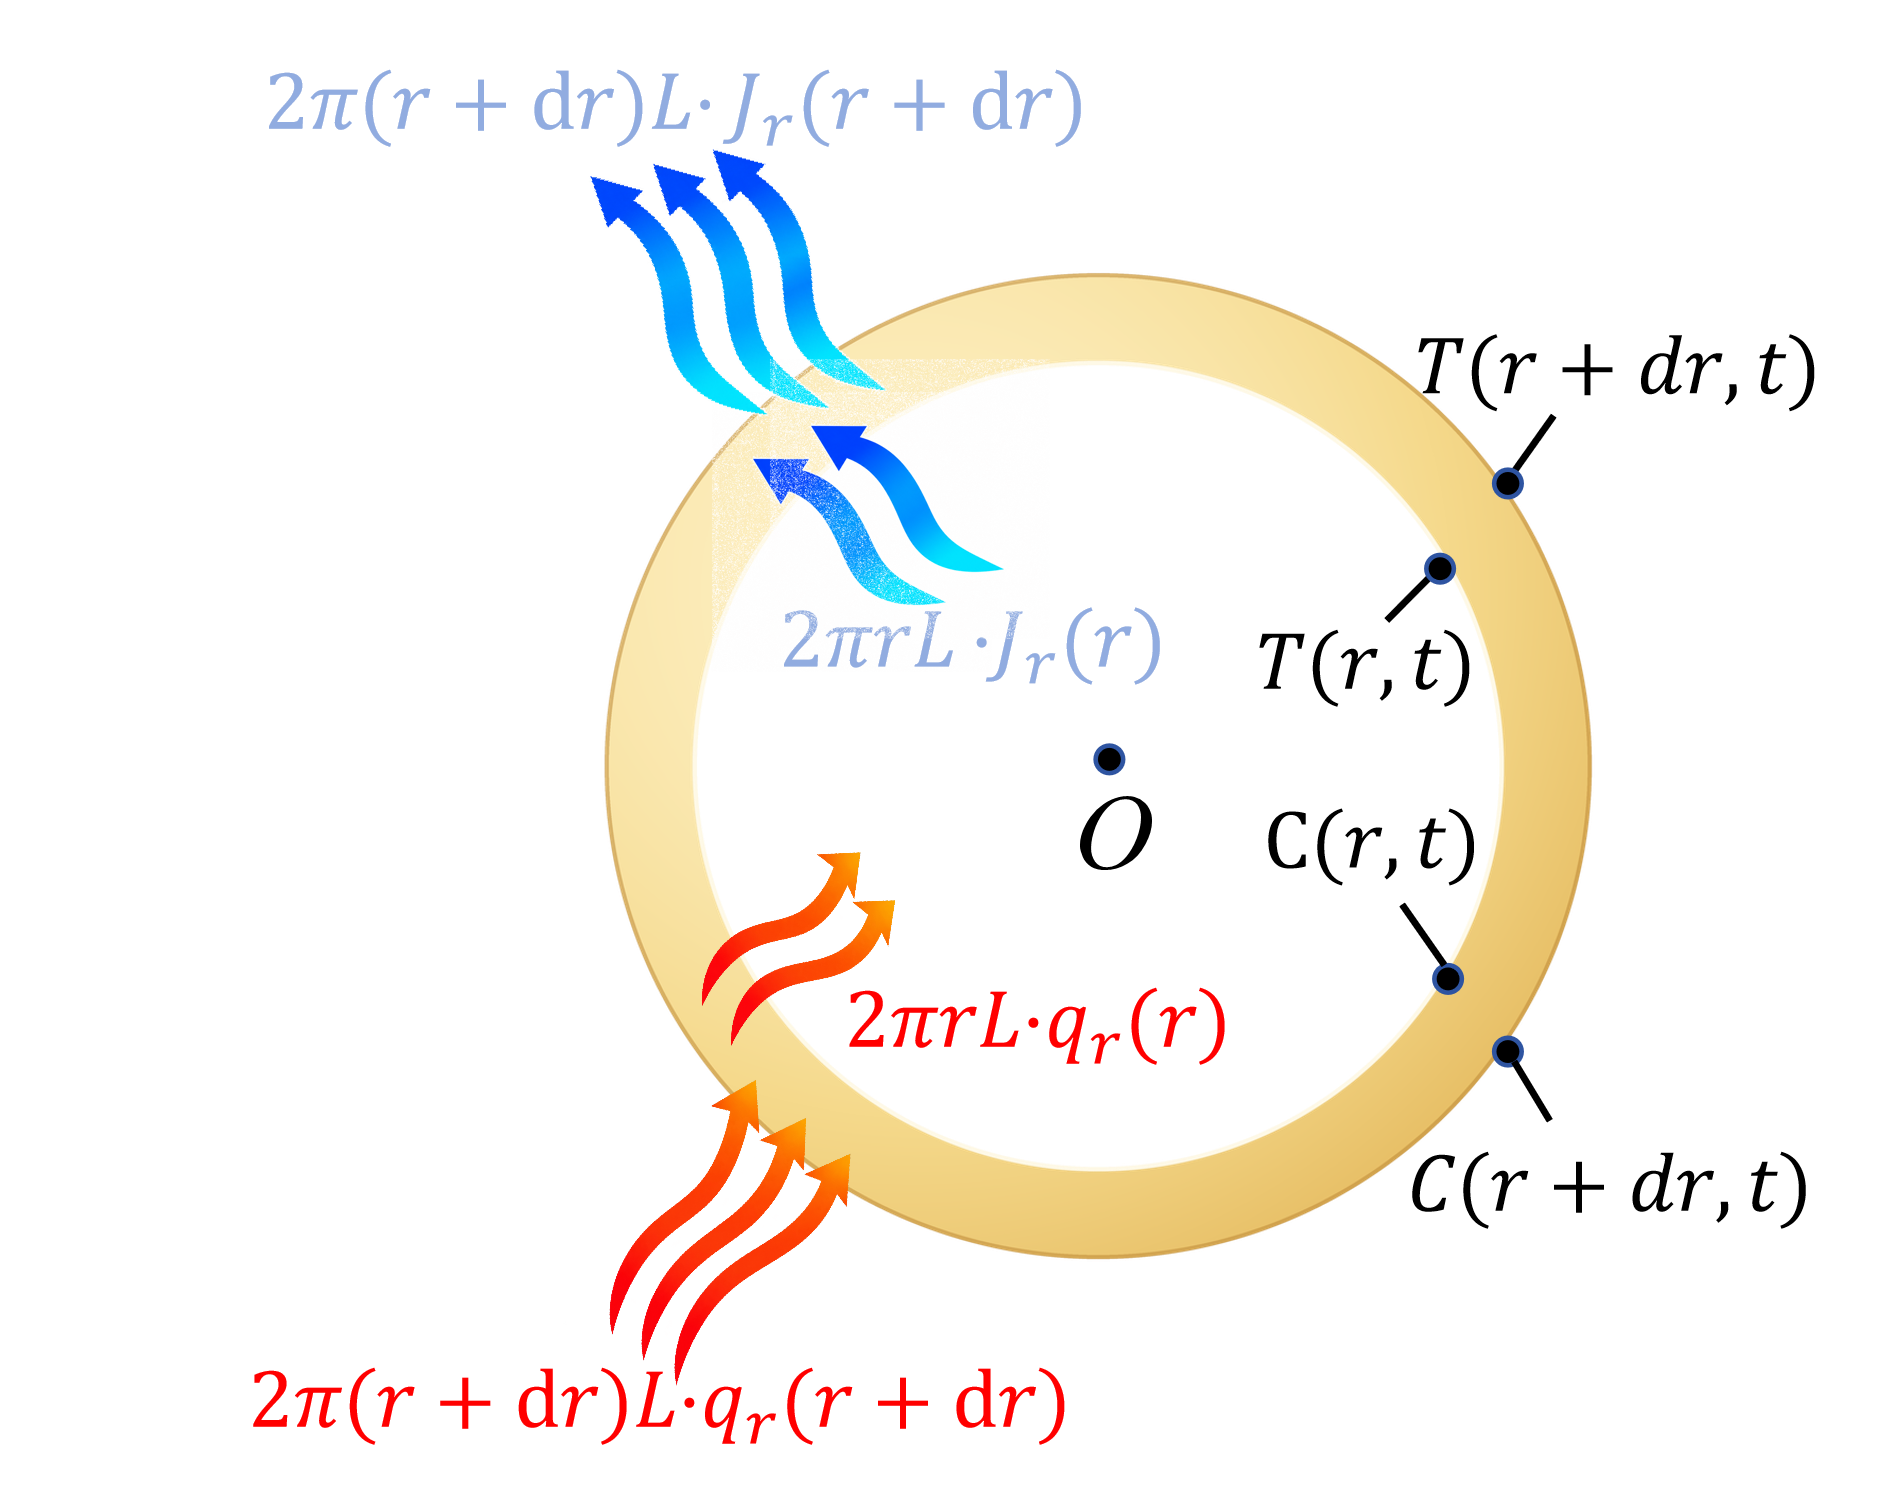
\includegraphics[width=0.8\textwidth]{figures/一维径向非稳态热传导示意图.png}
\caption{一维径向非稳态热传导和水分扩散示意图}
\label{fig:q1-radial-process}
\end{figure}

根据 Fourier 导热定律，药材内部的径向热流密度 $q_r$ 为 $-k\frac{\partial T}{\partial r}$。如图\ref{fig:q1-control-volume}所示，取半径为 $r$、厚度为 $\mathrm{d}r$、长度为 $L$ 的圆柱薄壳作为控制体，其体积 $\mathrm{d}V$为$2\pi rL\,\mathrm{d}r$。

\begin{figure}[H]
\centering
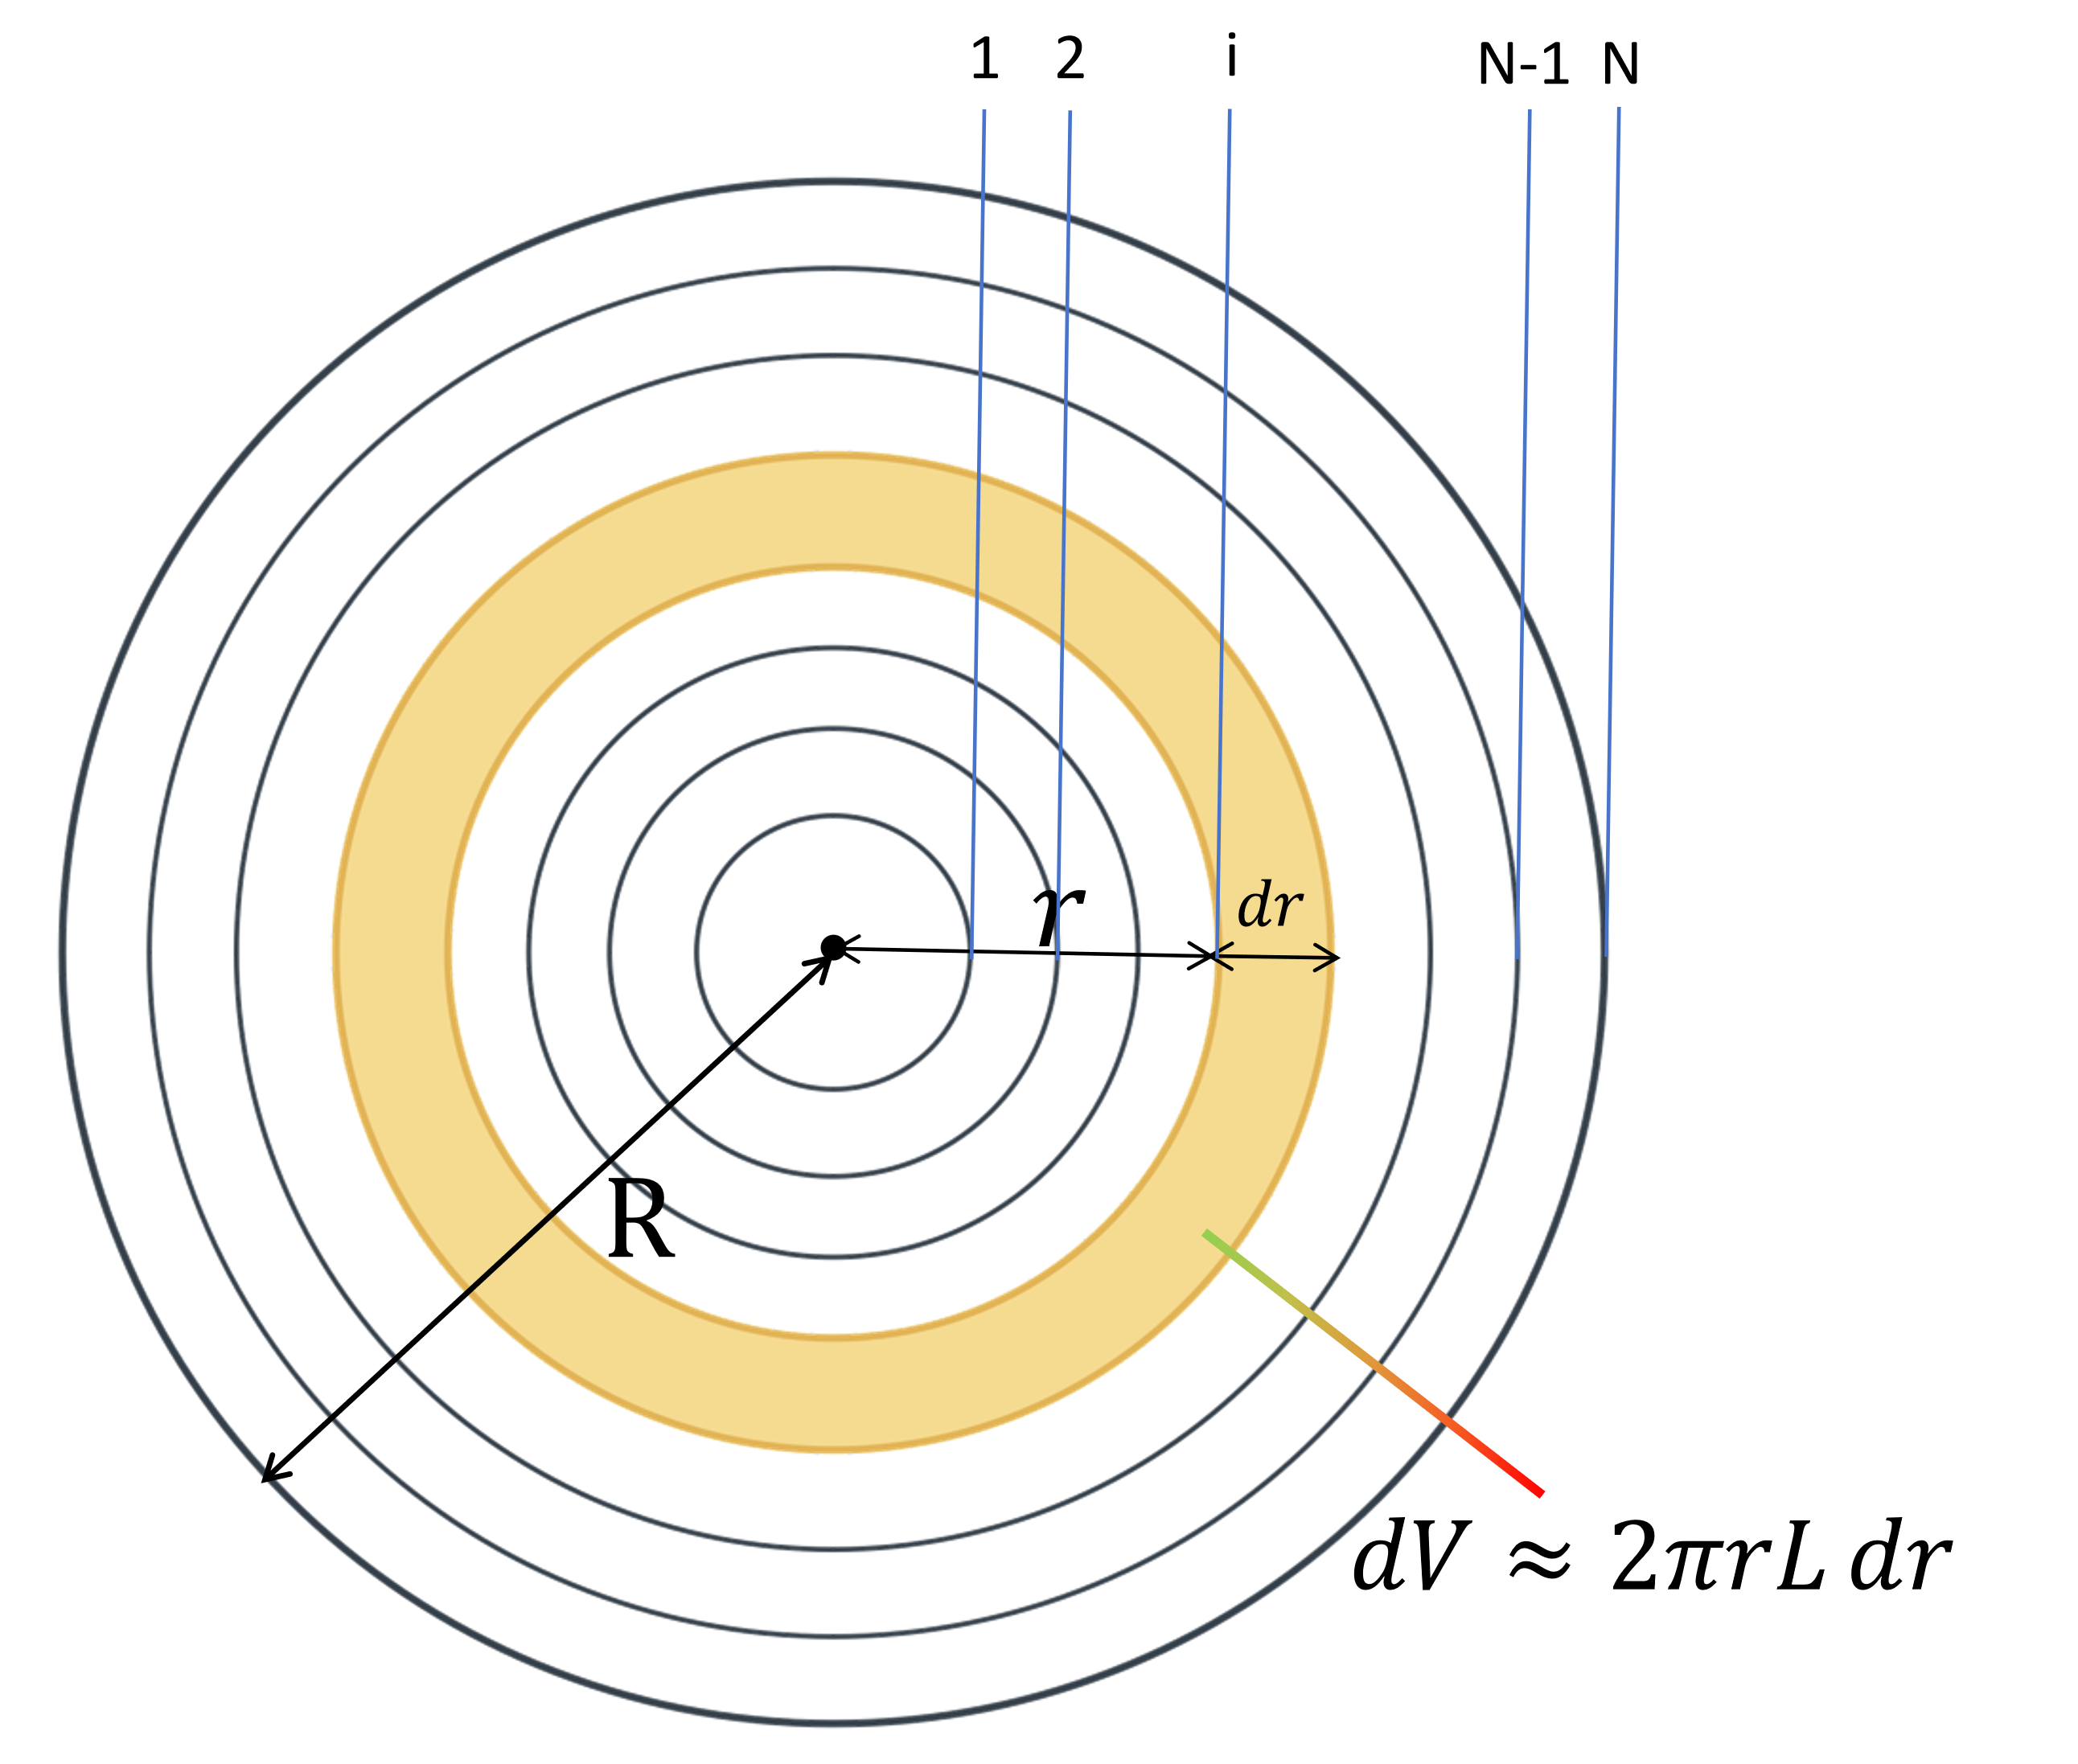
\includegraphics[width=0.8\textwidth]{figures/dV.png}
\caption{圆柱薄壳控制体示意图}
\label{fig:q1-control-volume}
\end{figure}

薄壳单位时间内的显热积累量为 $\rho c_p\,\mathrm{d}V\frac{\partial T}{\partial t}$。薄壳的净导热输入量等于内侧流入与外侧流出之差，由径向热流密度 $q_r$ 可写为 $-2\pi L\frac{\partial(rq_r)}{\partial r}\,\mathrm{d}r$。
根据能量守恒，显热积累量等于净导热输入量，约去公共因子 $2\pi L\,\mathrm{d}r$，得到圆柱坐标下的一维径向非稳态热传导方程：
\begin{equation}
\rho c_p\frac{\partial T}{\partial t}
=
\frac{1}{r}\frac{\partial}{\partial r}
\left(rk\frac{\partial T}{\partial r}\right)
\qquad 0<r<R,\quad 0<t\le1800\,\mathrm{s}.
\end{equation}
第一问中 $\rho$、$c_p$ 和 $k$ 均为常数，因此上式可写为：
\begin{equation}
\frac{\partial T}{\partial t}
=\alpha\left(
\frac{\partial^2T}{\partial r^2}
+\frac{1}{r}\frac{\partial T}{\partial r}
\right),
\qquad
\alpha=\frac{k}{\rho c_p}.
\end{equation}
代入题目给定的物性参数，得到热扩散率 $\alpha=1.6886\times10^{-7}\,\mathrm{m^2/s}$。

初始时刻，药材温度均匀分布，即$T(r,0)=28\,{}^\circ\mathrm{C}$。
由于圆柱中心满足轴对称条件，有 $\left.\frac{\partial T}{\partial r}\right|_{r=0}=0$。
令 $T_s=T(R,t)$，药材表面向外的导热通量$q_{\mathrm{out}}$为 $-k\left.\frac{\partial T}{\partial r}\right|_{r=R}$。
根据 Newton 对流换热定律，环境向表面传出的热流为 $h(T_\infty-T_s)$。在药材与烘房气体的分界面上，根据能量守恒原理，药材内部导热通量与界面对流换热通量相等，得到表面对流换热边界条件：
\begin{equation}
-k\left.\frac{\partial T}{\partial r}\right|_{r=R}
=h\left[T_s-T_\infty(t)\right].
  \label{eq:q1-surface-heat-flux}
\end{equation}

\subsubsection{水分场模型}
根据 Fick 第一定律\cite{fick1855}，药材内部的径向水分扩散通量 $J_r$ 为 $-D(C)\frac{\partial C}{\partial r}$。对同一圆柱薄壳控制体，含水率的积累量为 $2\pi rL\,\mathrm{d}r\frac{\partial C}{\partial t}$，水分的净扩散输入量为 $-2\pi L\frac{\partial(rJ_r)}{\partial r}\,\mathrm{d}r$。
根据质量守恒定律，约去公共因子并代入$J_r$，得到含水率的一维径向扩散方程
\begin{equation}
\frac{\partial C}{\partial t}
=
\frac{1}{r}\frac{\partial}{\partial r}
\left[rD(C)\frac{\partial C}{\partial r}\right]
\qquad 0<r<R,\quad 0<t\le1800\,\mathrm{s},
\end{equation}
其中水分扩散系数采用题目给定的经验公式：
\begin{equation}
D(C)=7\times10^{-9}
\exp\left(-\frac{0.89}{C}\right)\,\mathrm{m^2/s}.
\end{equation}

初始时刻，药材含水率均匀分布，即$C(r,0)=2.55$。令 $C_s=C(R,t)$。药材表面向外的扩散通量 $J_{\mathrm{out}}$ 为 $J_{\mathrm{out}}=-D(C_s)\left.\frac{\partial C}{\partial r}\right|_{r=R}$。根据线性对流传质定律，表面向环境传出的水分通量为 $h_m(C_s-C_\infty)$，故表面传质边界为
\begin{equation}
-D(C_s)\left.\frac{\partial C}{\partial r}\right|_{r=R}
=h_m\left[C_s-C_\infty(t)\right].
  \label{eq:q1-surface-moisture-flux}
\end{equation}

\subsubsection{数值离散与求解}

令径向步长为$\Delta r=0.1\,\mathrm{cm}$，时间步长为$\Delta t=1\,\mathrm{s}$，径向计算节点定义为：
\begin{equation}
\Delta r=0.1\,\mathrm{cm}=1.0\times10^{-3}\,\mathrm{m},
\qquad
r_i=i\Delta r,\quad i=0,1,\ldots,20
\label{eq:q1-space-grid}
\end{equation}

时间层定义为：
\begin{equation}
\Delta t=1\,\mathrm{s},
\qquad
t_n=n\Delta t
\label{eq:q1-time-grid}
\end{equation}
其中，$n$为时间层编号。


温度场和水分场均采用径向有限体积法离散，控制体取同心圆柱薄壳。为统一表示两个扩散方程，将其写为：
\begin{equation}
s\frac{\partial\phi}{\partial t}
=
\frac{1}{r}
\frac{\partial}{\partial r}
\left(
r\Gamma\frac{\partial\phi}{\partial r}
\right)
\label{eq:q1-unified-pde}
\end{equation}
其中，变量和参数对应关系为：
\begin{equation}
(\phi,s,\Gamma)=
\begin{cases}
(T,\rho c_p,k),&\text{温度场},\\
(C,1,D(C)),&\text{水分场}
\end{cases}
\label{eq:q1-unified-parameters}
\end{equation}

在每个时间层$t_n\rightarrow t_{n+1}$内，时间导数采用后向 Euler 全隐式离散，即$\partial\phi/\partial t\approx(\phi^{n+1}-\phi^n)/\Delta t$，离散方程中的未知量及传递系数均取$n+1$时刻。由式\eqref{eq:q1-unified-pde}和式\eqref{eq:q1-unified-parameters}在各径向控制体上的守恒积分，分别得到如下节点离散格式。

\paragraph{内部节点离散}
对内部节点$i=1,2,\ldots,N-1$，控制体的径向权重记为$M_i=r_i\Delta r$，并令$r_{i+\frac12}=r_i+\Delta r/2$。对统一控制方程进行积分并采用后向 Euler 格式，得到
\begin{equation}
s_iM_i\frac{\phi_i^{n+1}-\phi_i^n}{\Delta t}
=
r_{i+\frac12}\Gamma_{i+\frac12}^{n+1}
\frac{\phi_{i+1}^{n+1}-\phi_i^{n+1}}{\Delta r}
-r_{i-\frac12}\Gamma_{i-\frac12}^{n+1}
\frac{\phi_i^{n+1}-\phi_{i-1}^{n+1}}{\Delta r}
\label{eq:q1-fvm-interior}
\end{equation}
其中$N=20$，$s_i$为节点$r_i$处的储存系数，$\Gamma_{i+\frac12}^{n+1}$为界面$r_{i+\frac12}$处的传递系数。该式分别取$(\phi,s,\Gamma)=(T,\rho c_p,k)$和$(C,1,D(C))$时，对应温度场和水分场的内部节点离散方程。

\paragraph{中心节点离散}
中心控制体为$0\le r\le\Delta r/2$。利用圆柱中心的轴对称无通量条件，中心界面通量为零，从而避免直接计算统一控制方程中的$1/r$项，得到中心节点格式
\begin{equation}
s_0\frac{\phi_0^{n+1}-\phi_0^n}{\Delta t}
=\frac{4\Gamma_{\frac12}^{n+1}}{\Delta r^2}
\left(\phi_1^{n+1}-\phi_0^{n+1}\right)
\label{eq:q1-fvm-center}
\end{equation}

\paragraph{表面节点离散}
记表面节点为$N=20$，表面半控制体的径向权重为
\begin{equation}
M_N=\frac{R^2-(R-\Delta r/2)^2}{2}
\label{eq:q1-surface-weight}
\end{equation}
将前文的表面 Robin 边界通量式\eqref{eq:q1-surface-heat-flux}和式\eqref{eq:q1-surface-moisture-flux}代入表面控制体守恒式，得到统一的表面节点离散方程
\begin{equation}
sM_N\frac{\phi_N^{n+1}-\phi_N^n}{\Delta t}
=Rb\left(\phi_\infty^{n+1}-\phi_N^{n+1}\right)
-r_{N-\frac12}\Gamma_{N-\frac12}^{n+1}
\frac{\phi_N^{n+1}-\phi_{N-1}^{n+1}}{\Delta r}
\label{eq:q1-fvm-surface}
\end{equation}
其中$\phi_\infty^{n+1}$表示相应的环境温度或环境含水率，比例系数$b$为
\begin{equation}
b=
\begin{cases}
h,&\phi=T,\\
h_m,&\phi=C
\end{cases}
\label{eq:q1-surface-transfer-coefficient}
\end{equation}


\paragraph{非线性扩散系数处理}
由于水分扩散系数$D(C)$随含水率$C$非线性变化，水分场控制方程为非线性偏微分方程，故采用 Picard 迭代求解。温度方程中的$\rho$、$c_p$和$k$为常数，每个时间步可直接组装并求解一次线性三对角方程组。取上一时间层解$C^n$作为初始迭代值，在第$m$次迭代中根据$C_i^{(m)}$计算节点扩散系数
\begin{equation}
D_i^{(m)}=7\times10^{-9}\exp\left(-\frac{0.89}{C_i^{(m)}}\right)
\label{eq:q1-picard-diffusivity}
\end{equation}
界面扩散系数采用相邻节点扩散系数的调和平均
\begin{equation}
D_{i+\frac12}^{(m)}
=\frac{2D_i^{(m)}D_{i+1}^{(m)}}{D_i^{(m)}+D_{i+1}^{(m)}}
\label{eq:q1-harmonic-diffusivity}
\end{equation}
在固定$D^{(m)}$的条件下求解线性离散方程，得到新的含水率场$C^{(m+1)}$。当相邻两次迭代的最大绝对增量满足
\begin{equation}
\max_i\left|C_i^{(m+1)}-C_i^{(m)}\right|<10^{-10}
\label{eq:q1-picard-convergence}
\end{equation}
时，认为当前时间层收敛，并将收敛解作为下一时间层的初值。


\subsubsection{模型计算结果}

数值计算覆盖$t=0,1,\ldots,1800\,\mathrm{s}$的全部时间层和$r=0,0.1,\ldots,2.0\,\mathrm{cm}$的全部径向节点，完整计算结果保存于文件\texttt{result1.xlsx}。从数值解中提取$t=100,300,600,900,1200,1500,1800\,\mathrm{s}$时，$r=0,0.5,1.0,1.5,2.0\,\mathrm{cm}$处的温度和水分浓度，结果分别列于表2和表3。

\begin{table}[H]
\centering
\renewcommand{\arraystretch}{1.25}
{\centering\textbf{表2\quad 30分钟内药材的温度}\par}
\vspace{0.4em}
\begin{tabularx}{0.9\textwidth}{|>{\centering\arraybackslash}p{0.20\textwidth}|>{\centering\arraybackslash}X|>{\centering\arraybackslash}X|>{\centering\arraybackslash}X|>{\centering\arraybackslash}X|>{\centering\arraybackslash}X|}
\hline
\multirow{2}{*}{时间/s} & \multicolumn{5}{c|}{到药材中心的距离/cm} \\
\cline{2-6}
& 0 & 0.5 & 1 & 1.5 & 2 \\
\hline
100  & 28.0001 & 28.0003 & 28.0040 & 28.0327 & 28.1801 \\
\hline
300  & 28.0408 & 28.0635 & 28.1514 & 28.3681 & 28.8489 \\
\hline
600  & 28.4533 & 28.5360 & 28.8039 & 29.3159 & 30.1652 \\
\hline
900  & 29.3243 & 29.4583 & 29.8755 & 30.6161 & 31.7304 \\
\hline
1200 & 30.5427 & 30.7098 & 31.2223 & 32.1126 & 33.4276 \\
\hline
1500 & 31.9957 & 32.1867 & 32.7660 & 33.7463 & 35.1203 \\
\hline
1800 & 33.5753 & 33.7720 & 34.3642 & 35.3621 & 36.7856 \\
\hline
\end{tabularx}
\end{table}

\begin{table}[H]
\centering
\renewcommand{\arraystretch}{1.25}
{\centering\textbf{表3\quad 30分钟内药材的水分浓度}\par}
\vspace{0.4em}
\begin{tabularx}{0.9\textwidth}{|>{\centering\arraybackslash}p{0.20\textwidth}|>{\centering\arraybackslash}X|>{\centering\arraybackslash}X|>{\centering\arraybackslash}X|>{\centering\arraybackslash}X|>{\centering\arraybackslash}X|}
\hline
\multirow{2}{*}{时间/s} & \multicolumn{5}{c|}{到药材中心的距离/cm} \\
\cline{2-6}
& 0 & 0.5 & 1 & 1.5 & 2 \\
\hline
100  & 2.5500 & 2.5500 & 2.5500 & 2.5500 & 2.2470 \\
\hline
300  & 2.5500 & 2.5500 & 2.5500 & 2.5492 & 2.0508 \\
\hline
600  & 2.5500 & 2.5500 & 2.5500 & 2.5353 & 1.8770 \\
\hline
900  & 2.5500 & 2.5500 & 2.5497 & 2.5045 & 1.7547 \\
\hline
1200 & 2.5500 & 2.5500 & 2.5482 & 2.4646 & 1.6586 \\
\hline
1500 & 2.5500 & 2.5499 & 2.5445 & 2.4206 & 1.5787 \\
\hline
1800 & 2.5500 & 2.5497 & 2.5383 & 2.3755 & 1.5102 \\
\hline
\end{tabularx}
\end{table}\

\noindent


图\ref{fig:q1-3d-surfaces}和图\ref{fig:q1-clouds}分别以三维时空曲面和分时刻云图的形式展示了温度场与水分浓度场的分布特征。其中，图7(a)和(b)分别为温度场和水分浓度场的三维时空分布曲面图；图\ref{fig:q1-clouds}(a)和(b)分别为$t=0\,\mathrm{s}$、$900\,\mathrm{s}$和$1800\,\mathrm{s}$时刻的温度场和水分浓度场分布云图。

\begin{figure}[H]
\centering
\begin{subfigure}[b]{0.48\textwidth}
\centering
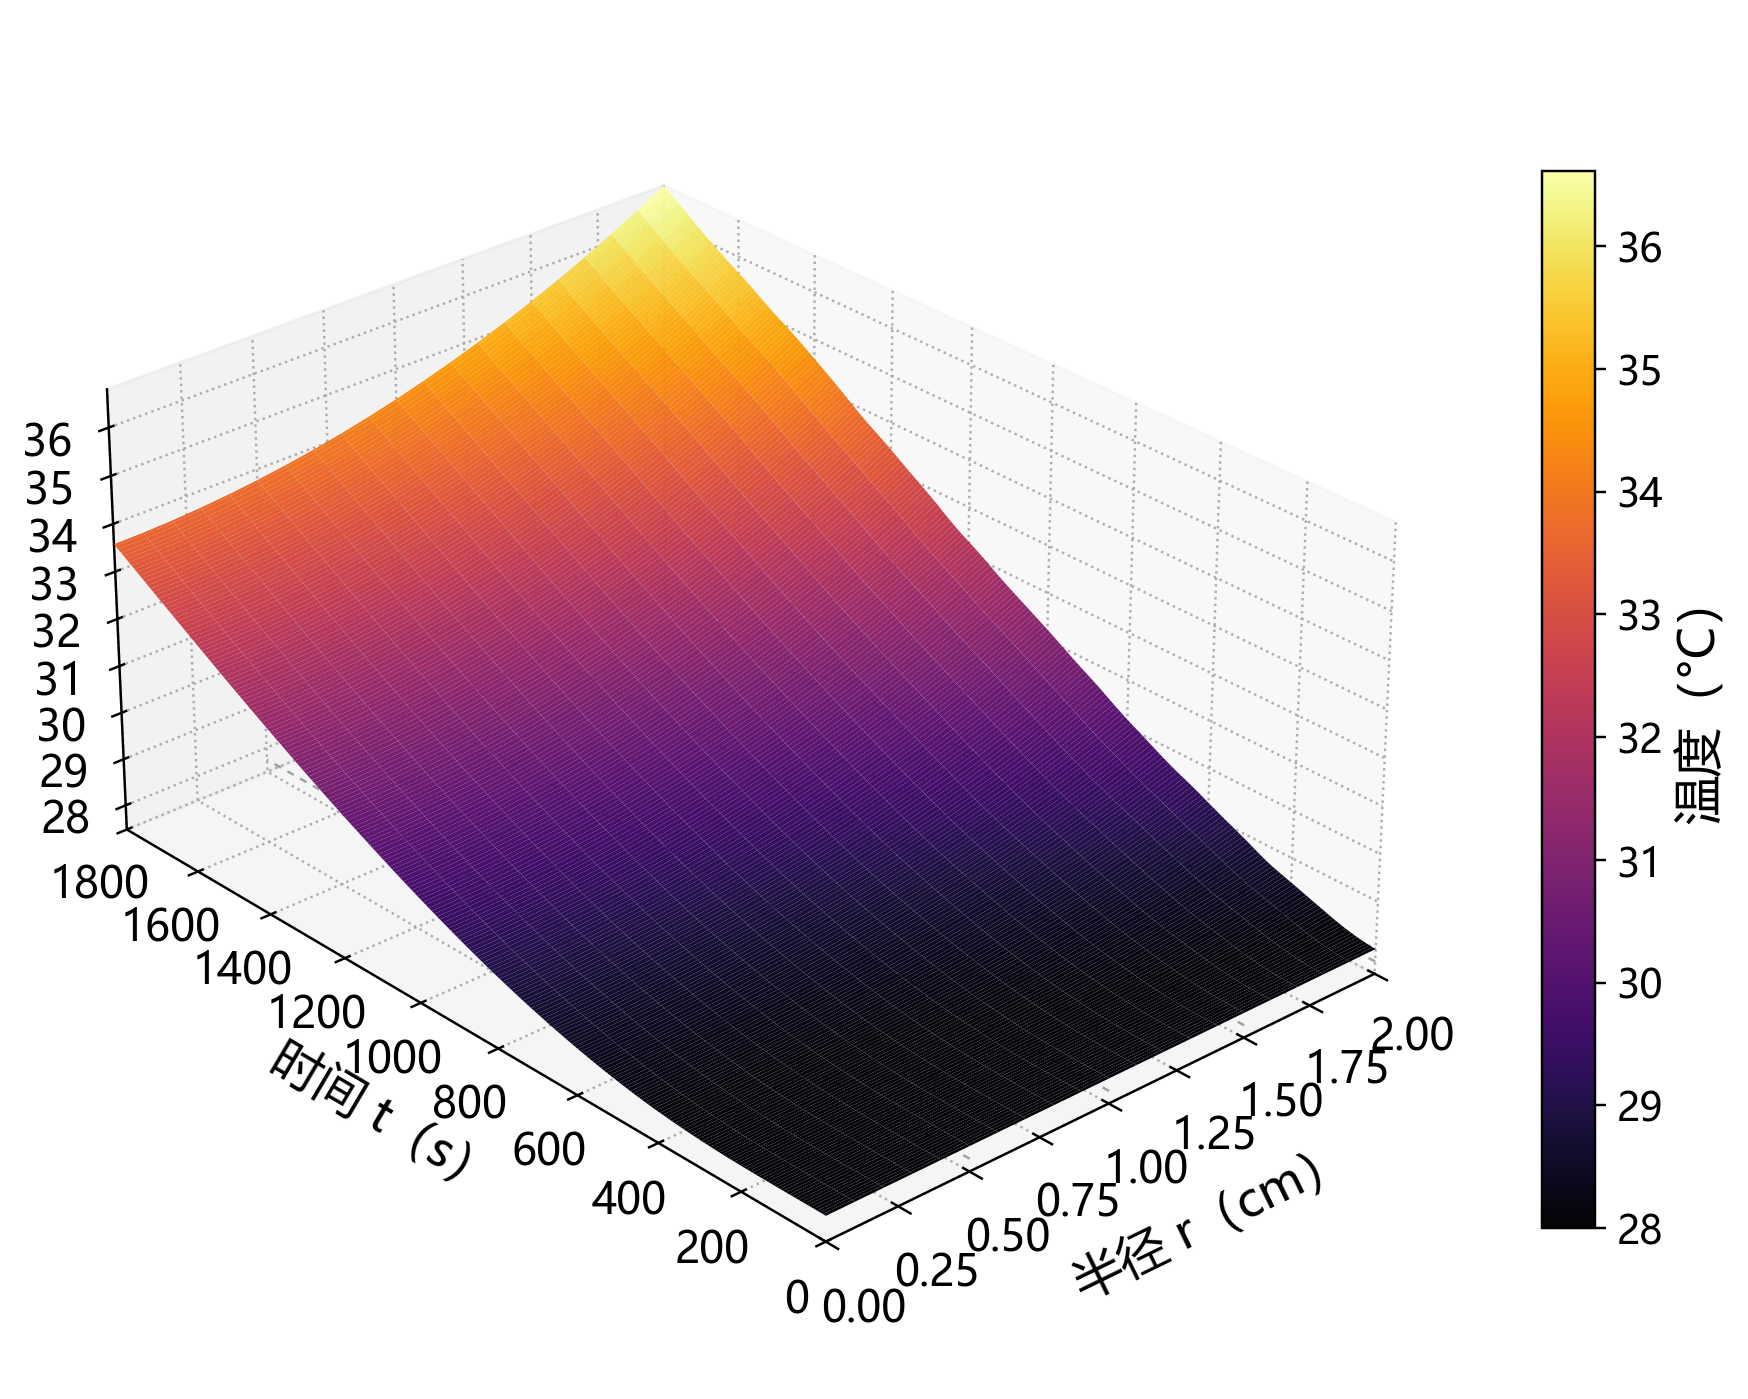
\includegraphics[width=\linewidth]{figures/温度三维时空分布曲面图.png}
\caption{温度三维时空分布曲面图}
\label{fig:q1-temperature-surface}
\end{subfigure}
\hfill
\begin{subfigure}[b]{0.48\textwidth}
\centering
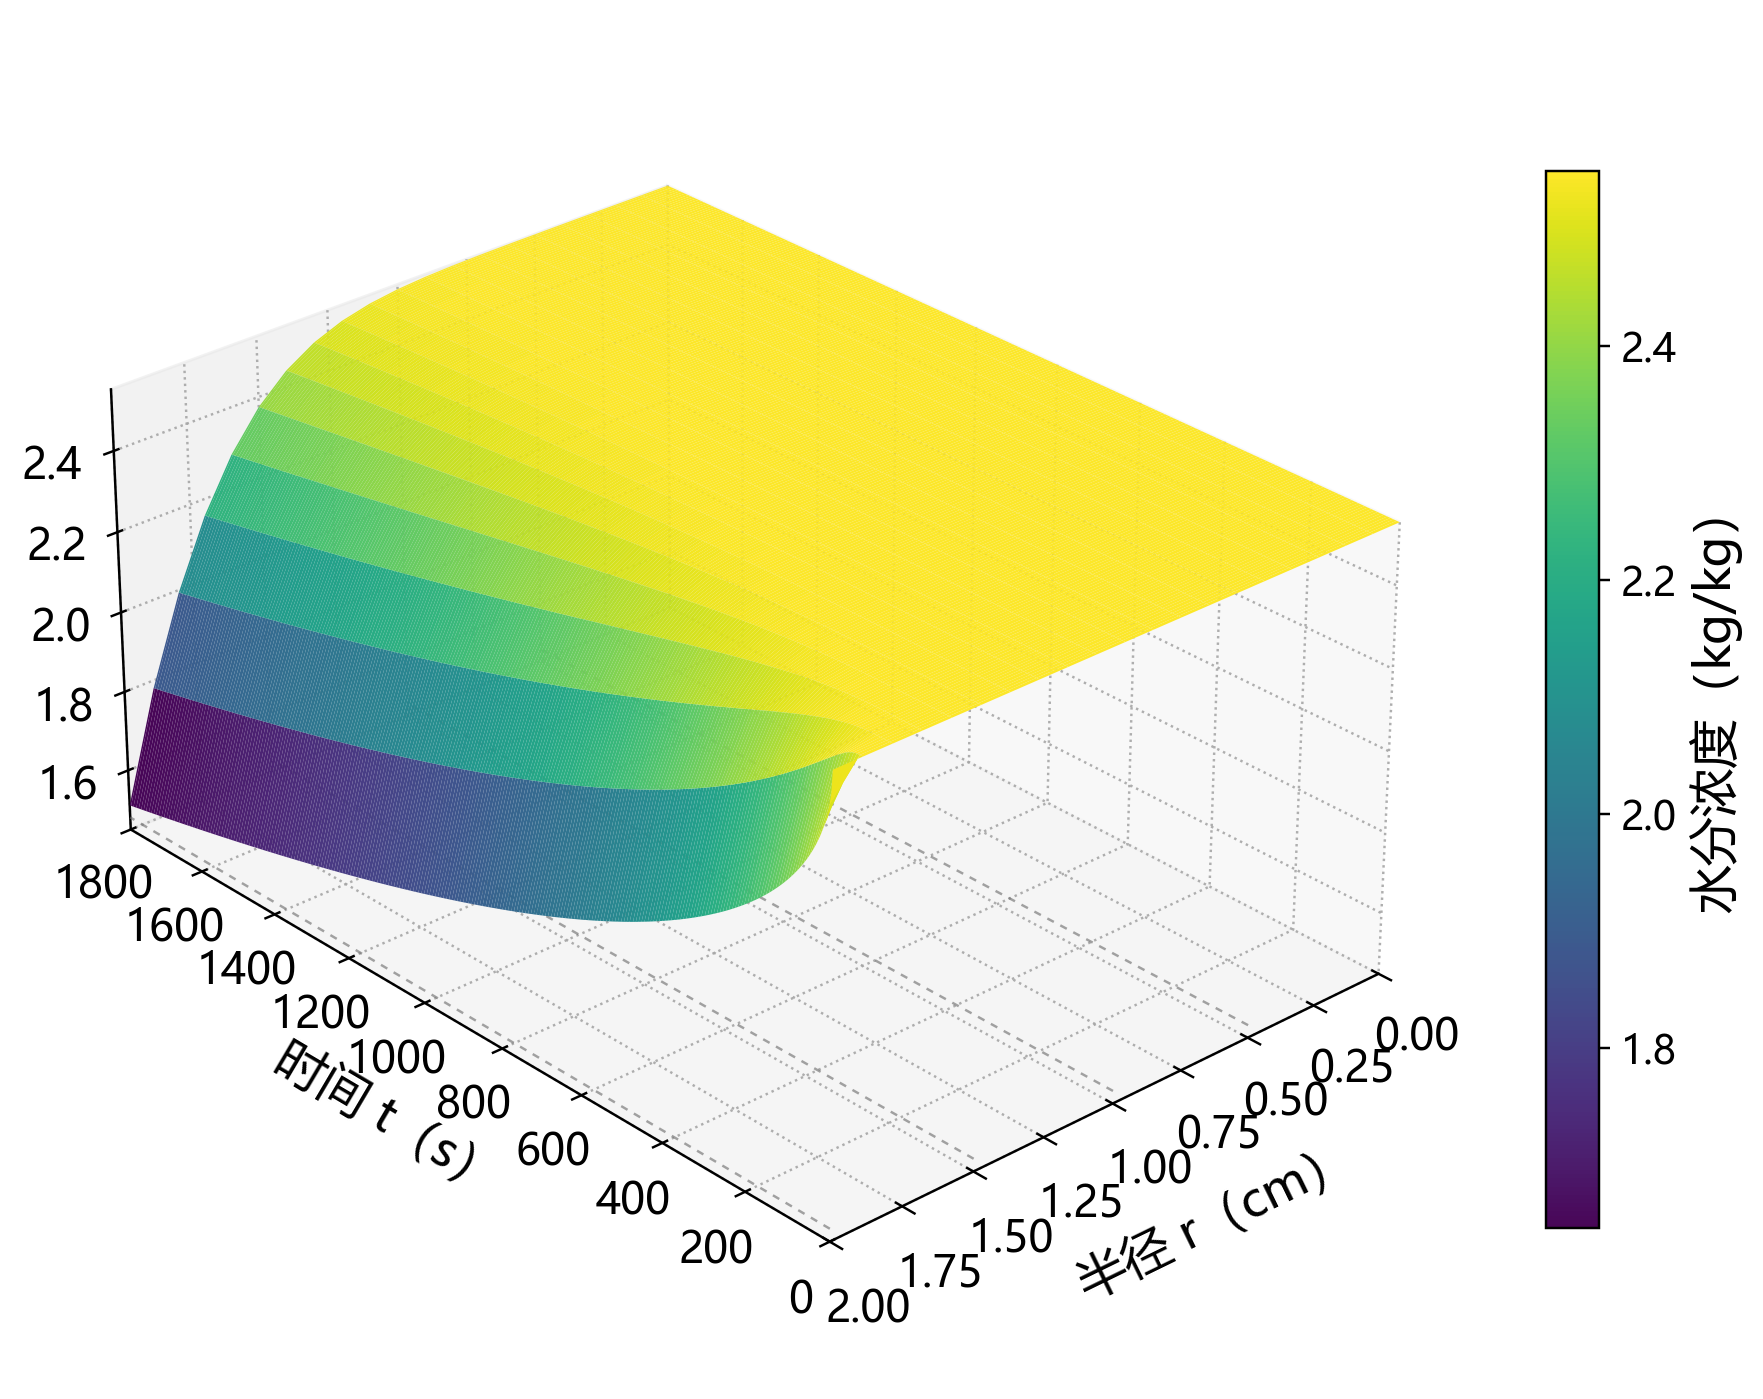
\includegraphics[width=\linewidth]{figures/水分浓度三维时空分布曲面图.png}
\caption{水分浓度三维时空分布曲面图}
\label{fig:q1-moisture-surface}
\end{subfigure}
\caption{温度和水分浓度三维时空分布曲面图}
\label{fig:q1-3d-surfaces}
\end{figure}

\begin{figure}[H]
\centering
\begin{subfigure}[b]{0.48\textwidth}
\centering
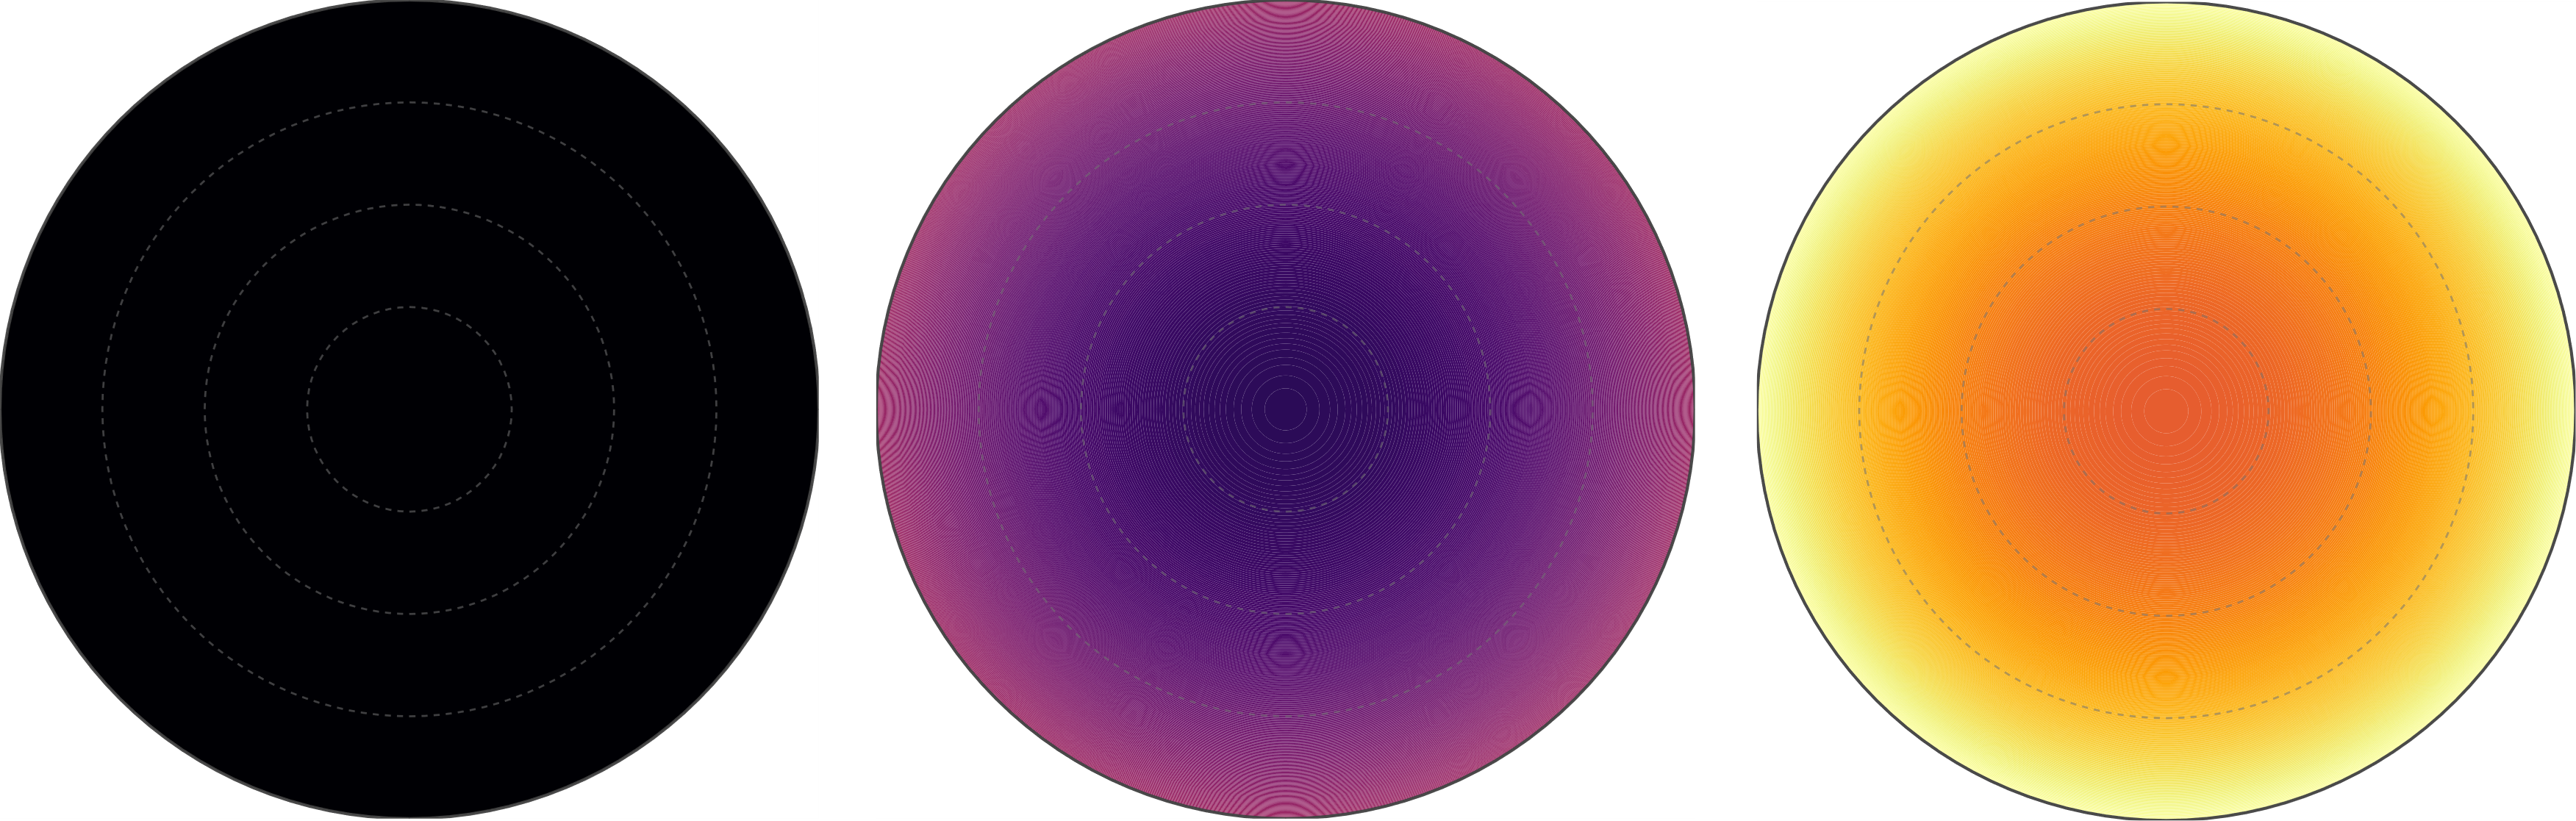
\includegraphics[width=\linewidth]{figures/云A.png}
\caption{$t=0\,\mathrm{s}$、$900\,\mathrm{s}$和$1800\,\mathrm{s}$时刻的温度分布云图}
\label{fig:q1-temperature-clouds}
\end{subfigure}
\hfill
\begin{subfigure}[b]{0.48\textwidth}
\centering
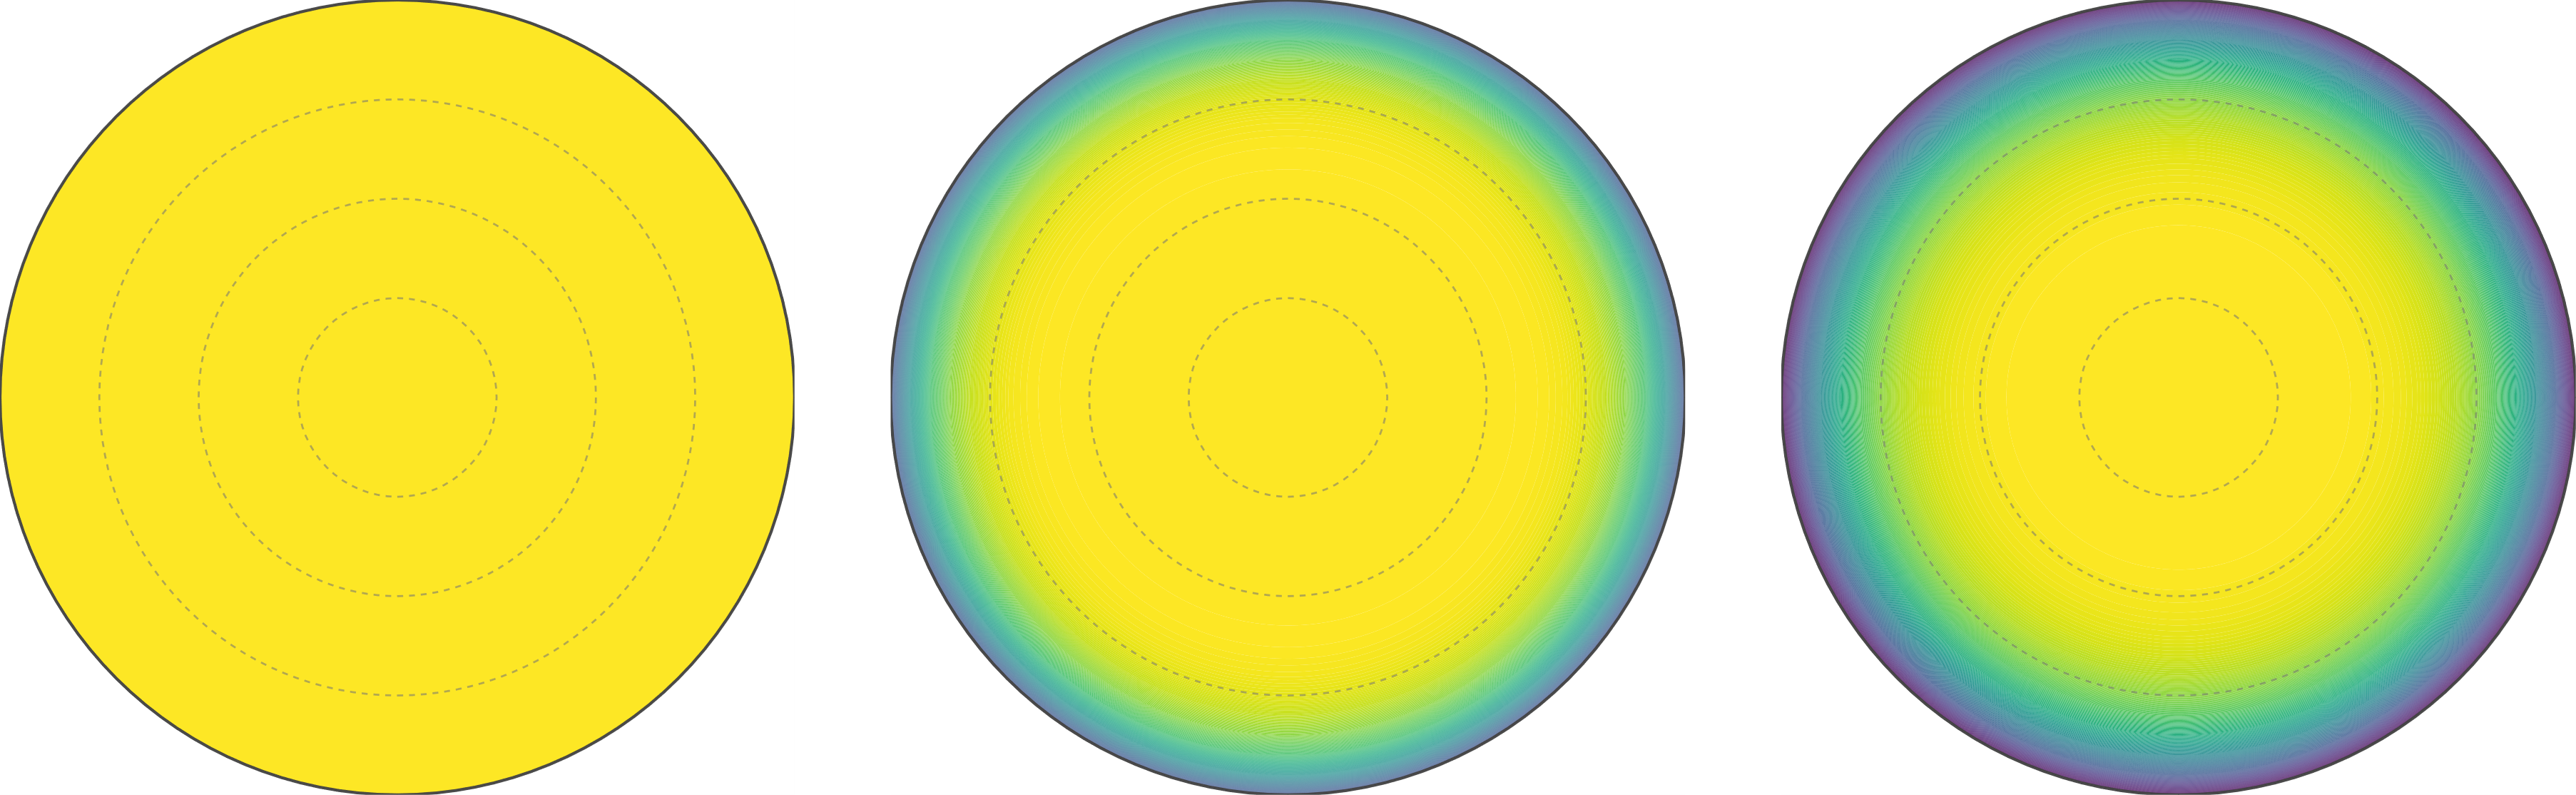
\includegraphics[width=\linewidth]{figures/云B.png}
\caption{$t=0\,\mathrm{s}$、$900\,\mathrm{s}$和$1800\,\mathrm{s}$时刻的水分浓度分布云图}
\label{fig:q1-moisture-clouds}
\end{subfigure}
\caption{不同时间的温度和水分浓度分布云图}
\label{fig:q1-clouds}
\end{figure}

\subsection{问题二模型的建立与求解}

\subsubsection{问题二模型的更新}

问题二沿用问题一建立的一维径向非稳态“传热-传质”模型，进一步考虑药材物性参数随温度和含水率变化的影响。并且，如图\ref{fig:q1-drying-process}所示,问题二将研究过程拓展到了整个烘干过程，分为预热平衡与恒温干燥阶段。其中，密度、比热容和导热系数随含水率变化，水分扩散系数同时受含水率和温度影响。因此，含水率场通过改变密度、比热容和导热系数影响温度场，温度场又通过扩散系数影响水分场，二者构成双向耦合的关系。

\begin{figure}[H]
\centering
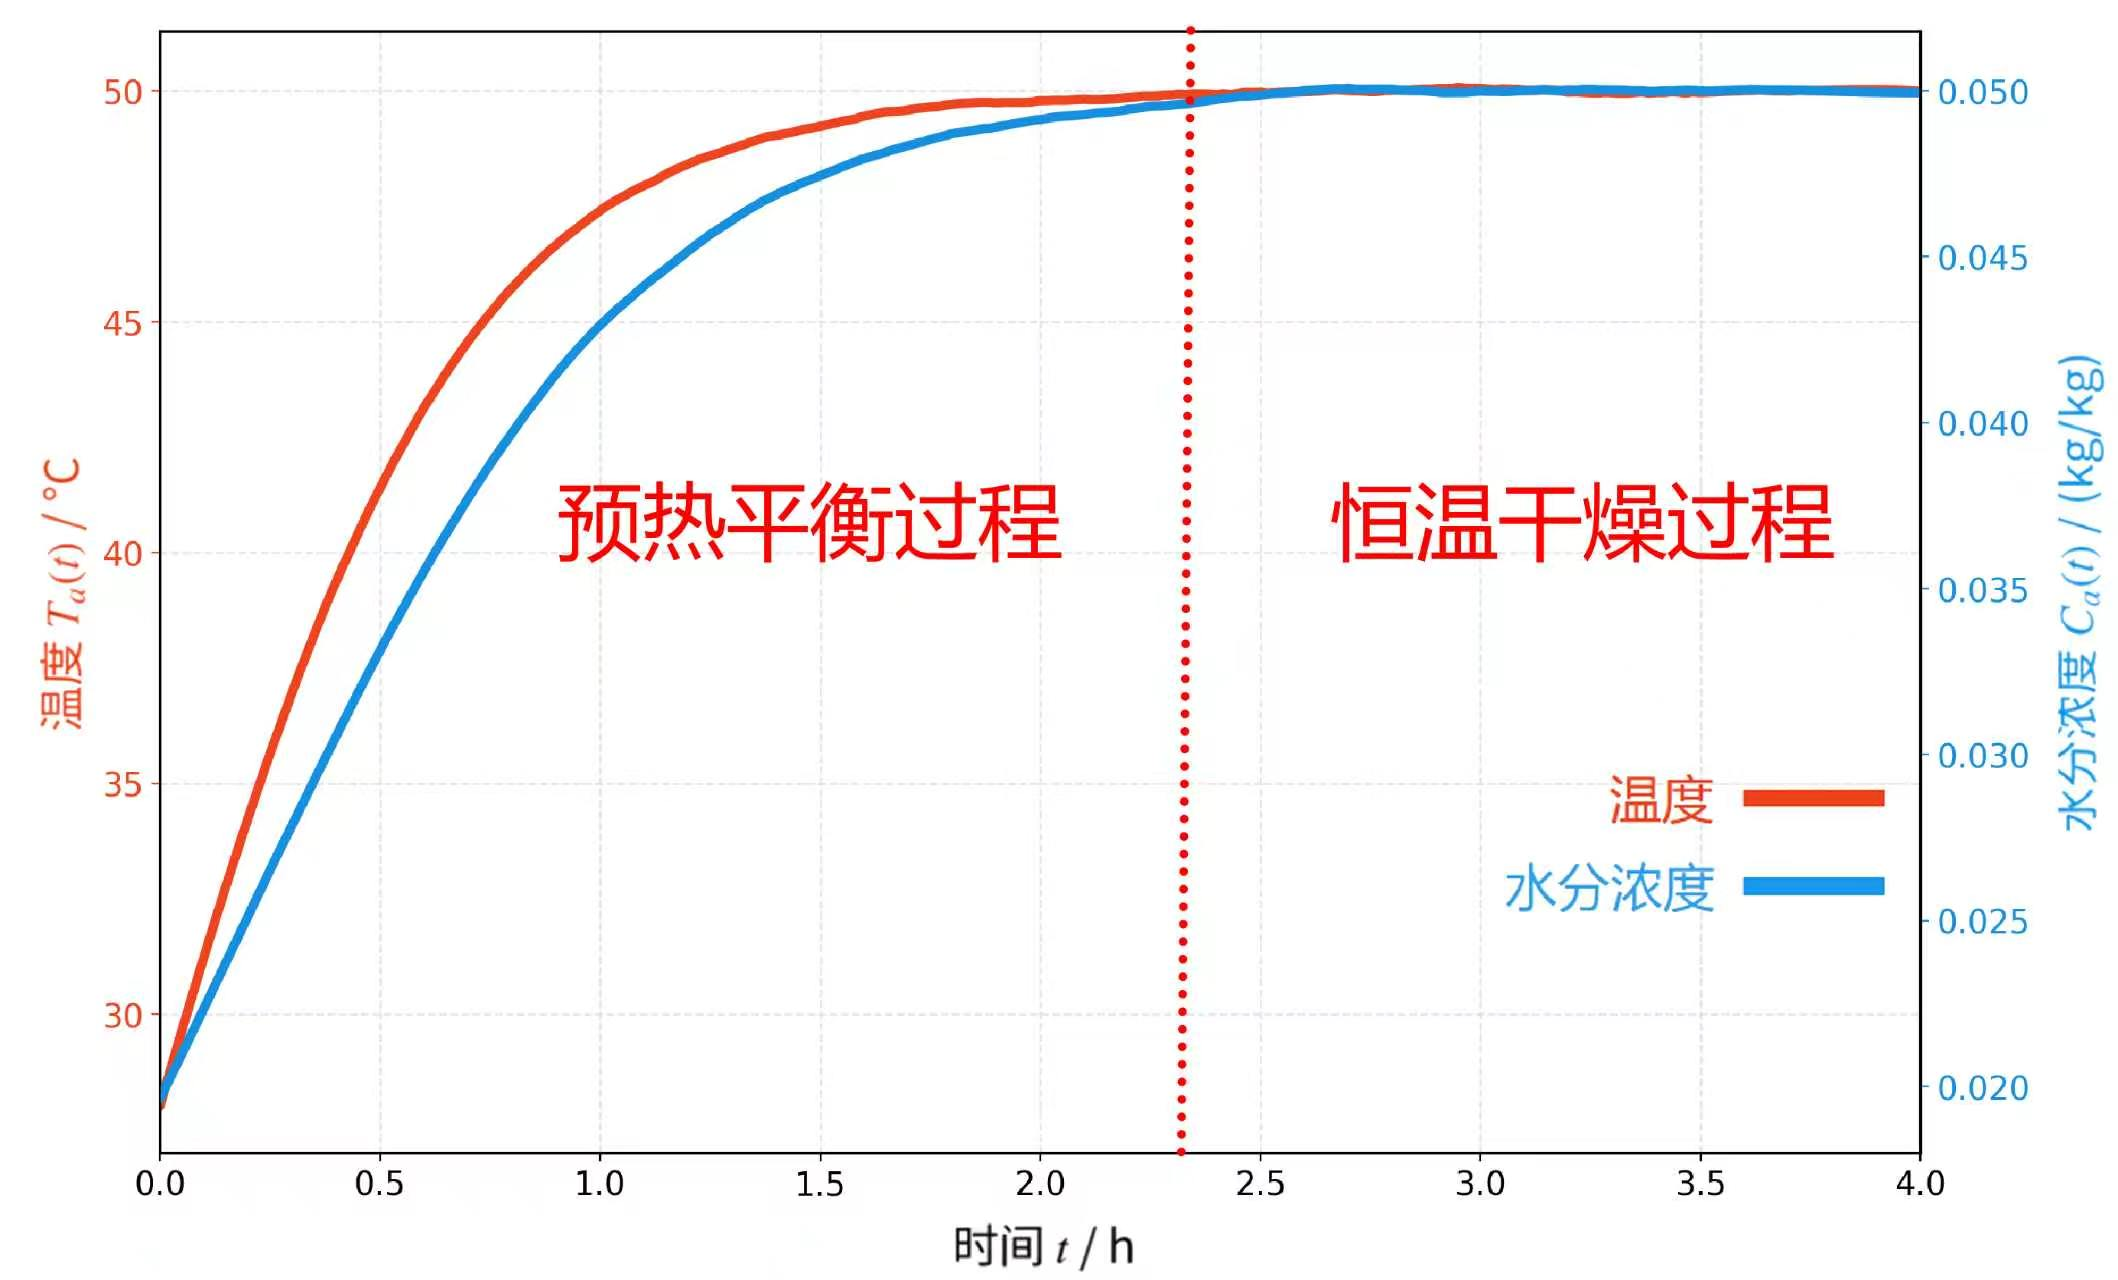
\includegraphics[width=0.8\textwidth]{figures/药材烘干过程示意图.png}
\caption{药材预热烘干过程示意图}
\label{fig:q1-drying-process}
\end{figure}

\subsubsection{变物性热湿耦合方程}

根据附录3，药材的变物性参数统一表示为
\begin{equation}
\left\{
\begin{aligned}
\rho(C)&=650+128C,\\
c_p(C)&=1450+2736\frac{C}{C+1},\\
k(C)&=0.21+0.38\frac{C}{C+1},\\
D(C,T_K)&=2.4\times10^{-3}
\exp\left(-\frac{0.45}{C}\right)
\exp\left(-\frac{3850}{T_K}\right)
\end{aligned}
\right.
\label{eq:q2-variable-properties}
\end{equation}
其中，$\rho$、$c_p$和$k$分别表示密度、比热容和导热系数，$D$表示水分扩散系数，$T_K$为绝对温度。
扩散系数公式中的温度采用绝对温度，因此计算时使用：
\begin{equation}
T_K=T+273.15
\label{eq:q2-absolute-temperature}
\end{equation}

将上述变物性关系代入能量守恒方程和质量守恒方程，得到问题二的温度场控制方程：
\begin{equation}
\boxed{
\rho(C)c_p(C)\frac{\partial T}{\partial t}
=
\frac{1}{r}
\frac{\partial}{\partial r}
\left[
rk(C)\frac{\partial T}{\partial r}
\right]
}
\label{eq:q2-variable-heat}
\end{equation}
以及水分场控制方程：
\begin{equation}
\boxed{
\frac{\partial C}{\partial t}
=
\frac{1}{r}
\frac{\partial}{\partial r}
\left[
rD(C,T_K)\frac{\partial C}{\partial r}
\right]
}
\label{eq:q2-variable-moisture}
\end{equation}

含水率$C$决定$\rho(C)$、$c_p(C)$和$k(C)$，而温度$T$与含水率$C$共同决定扩散系数$D(C,T_K)$。因此，温度场和水分场需要在同一时间层内迭代求解。

\subsubsection{数值离散与耦合求解}

\paragraph{非均匀网格的构造思想}
药材内部的温度和含水率主要通过表面与烘房交换。表面 Robin 边界直接施加热量和水分通量，烘干初期在表面附近形成比内部更陡的径向梯度。若全域采用能够分辨该边界层的均匀细网格，会在梯度较缓的内部区域产生大量冗余节点；若仅按$0.1\,\mathrm{cm}$输出间距离散，又不足以准确计算表面梯度和边界通量。为兼顾表面分辨率与计算效率，本文采用“内部较疏、表面加密”的两区节点型有限体积网格。

设药材半径为$R=0.02\,\mathrm{m}$，表面加密层厚度为$\delta_s=0.002\,\mathrm{m}$，内部网格步长为$\Delta r_b$，表面网格步长为$\Delta r_s$，加密倍率取$q=10$，即
\begin{equation}
\Delta r_s=\frac{\Delta r_b}{q}.
\label{eq:q2-grid-ratio}
\end{equation}
径向区间总数取$N=760$。由两区的区间数之和满足
\begin{equation}
\frac{R-\delta_s}{\Delta r_b}
+
\frac{\delta_s}{\Delta r_s}
=N,
\label{eq:q2-grid-count}
\end{equation}
得到
\begin{equation}
\Delta r_b
=
\frac{(R-\delta_s)+q\delta_s}{N}
=5.0\times10^{-5}\,\mathrm{m}
=50\,\mu\mathrm{m},
\qquad
\Delta r_s
=5.0\times10^{-6}\,\mathrm{m}
=5\,\mu\mathrm{m}.
\label{eq:q2-grid-steps}
\end{equation}
因此，$0\le r\le1.8\,\mathrm{cm}$的内部区域含$360$个区间，$1.8\,\mathrm{cm}<r\le2.0\,\mathrm{cm}$的表面层含$400$个区间，共有$N+1=761$个计算节点。节点坐标写为
\begin{equation}
r_i=
\begin{cases}
i\Delta r_b,
&0\le i\le360,\\
R-\delta_s+(i-360)\Delta r_s,
&360\le i\le760.
\end{cases}
\label{eq:q2-grid-nodes}
\end{equation}
该网格在仅使用$760$个区间的情况下获得$5\,\mu\mathrm{m}$的表面分辨率；若全域均采用同样的$5\,\mu\mathrm{m}$步长，则需要$4000$个区间。两区网格由此减少约$81\%$的空间未知量，同时保留最需要加密的表面区域。题目要求的$r=0,0.1,\ldots,2.0\,\mathrm{cm}$均为上述网格的实际节点，故结果输出不需要额外空间插值。

\paragraph{非均匀网格上的有限体积离散}
记相邻节点中点为控制面
\begin{equation}
r_{i+\frac12}=\frac{r_i+r_{i+1}}{2}.
\label{eq:q2-control-faces}
\end{equation}
约去所有控制体共有的$2\pi L$后，中心、内部和表面节点的径向体积权重分别为
\begin{equation}
M_0=\frac{r_{\frac12}^2}{2},
\qquad
M_i=\frac{r_{i+\frac12}^2-r_{i-\frac12}^2}{2},
\qquad
M_N=\frac{R^2-r_{N-\frac12}^2}{2}.
\label{eq:q2-control-weights}
\end{equation}
为统一表示温度场和水分场，定义
\begin{equation}
(\phi,S_i,\Gamma_i,b)=
\begin{cases}
\bigl(T,\rho(C_i)c_p(C_i),k(C_i),h\bigr),
&\text{温度场},\\
\bigl(C,1,D(C_i,T_i+273.15),h_m\bigr),
&\text{水分场}.
\end{cases}
\label{eq:q2-unified-parameters}
\end{equation}
界面传递系数采用相邻节点值的调和平均
\begin{equation}
\Gamma_{i+\frac12}
=
\frac{2\Gamma_i\Gamma_{i+1}}{\Gamma_i+\Gamma_{i+1}},
\label{eq:q2-harmonic-coefficient}
\end{equation}
并定义界面导通系数
\begin{equation}
G_{i+\frac12}
=
\frac{r_{i+\frac12}\Gamma_{i+\frac12}}
{r_{i+1}-r_i}.
\label{eq:q2-face-conductance}
\end{equation}
由控制体守恒积分，内部节点$i=1,\ldots,N-1$满足
\begin{equation}
S_iM_i\frac{\mathrm d\phi_i}{\mathrm dt}
=
G_{i+\frac12}(\phi_{i+1}-\phi_i)
-G_{i-\frac12}(\phi_i-\phi_{i-1}).
\label{eq:q2-fvm-interior}
\end{equation}
圆心处利用轴对称无通量条件，得到
\begin{equation}
S_0M_0\frac{\mathrm d\phi_0}{\mathrm dt}
=
G_{\frac12}(\phi_1-\phi_0),
\label{eq:q2-fvm-center}
\end{equation}
从而不需要在$r=0$处直接计算$1/r$。表面控制体计入 Robin 边界通量：
\begin{equation}
S_NM_N\frac{\mathrm d\phi_N}{\mathrm dt}
=
Rb\bigl(\phi_\infty(t)-\phi_N\bigr)
-G_{N-\frac12}(\phi_N-\phi_{N-1}).
\label{eq:q2-fvm-surface}
\end{equation}
上述形式在网格疏密交界面仍保持逐控制体守恒，非均匀间距通过$M_i$和$G_{i+\frac12}$直接进入离散方程。

\paragraph{半离散耦合系统与自适应 BDF}
将全部温度和含水率节点排列为
\begin{equation}
\boldsymbol y
=
\left(
T_0,\ldots,T_N,
C_0,\ldots,C_N
\right)^{\mathsf T}
\in\mathbb R^{1522},
\label{eq:q2-state-vector}
\end{equation}
由式\eqref{eq:q2-fvm-interior}--\eqref{eq:q2-fvm-surface}得到刚性非线性常微分方程组
\begin{equation}
\frac{\mathrm d\boldsymbol y}{\mathrm dt}
=
\boldsymbol F(t,\boldsymbol y).
\label{eq:q2-semidiscrete-system}
\end{equation}
每次计算$\boldsymbol F$时，由当前$\boldsymbol y$同步更新$\rho(C)$、$c_p(C)$、$k(C)$和$D(C,T_K)$，再计算热量与水分的界面净通量。因此，第二问是由隐式求解器对$1522$个未知量整体处理其非线性耦合。

时间积分采用自适应变阶 BDF。对第$n+1$个内部时间步，其一般形式可表示为
\begin{equation}
\sum_{j=0}^{q_n}
\alpha_{j,n}\boldsymbol y_{n+1-j}
=
\Delta t_n\beta_n
\boldsymbol F(t_{n+1},\boldsymbol y_{n+1}),
\qquad
1\le q_n\le5,
\label{eq:q2-adaptive-bdf}
\end{equation}
其中阶数$q_n$和内部步长$\Delta t_n$由局部误差估计自动调整。温度和含水率量纲不同，故分别设置绝对容差；主计算参数为
\begin{equation}
\operatorname{rtol}=2\times10^{-9},
\qquad
\operatorname{atol}_T=2\times10^{-9},
\qquad
\operatorname{atol}_C=2\times10^{-11}.
\label{eq:q2-bdf-tolerances}
\end{equation}
初始内部时间步取$10^{-4}\,\mathrm{s}$，最大内部时间步限制为$5\,\mathrm{s}$。求解器在相邻输出时刻之间可根据误差自动细分时间步。

由于每个节点只与自身及相邻节点的温度、含水率有关，系统 Jacobian 呈块三对角稀疏结构。计算中预先提供这一稀疏结构，以降低数值 Jacobian 计算和隐式线性方程组分解的开销，但不改变控制方程和误差判据。

\paragraph{网格与时间误差验证}
为检验非均匀网格的充分性，保持表面加密层厚度和$10$倍加密比例不变，依次采用$N=190,380,760$进行空间加密。由三层结果得到的温度、含水率最大范数观测阶分别为$1.8790$和$1.9999$，细网格的$1.25$倍 Richardson 安全误差上界分别为$4.665153\times10^{-6}\,{}^\circ\mathrm C$和$1.455194\times10^{-5}\,\mathrm{kg/kg}$。在$N=760$上进一步将积分容差缩小$4$倍并把最大内部步长减至$2.5\,\mathrm{s}$，温度和含水率最大变化分别为$5.360042\times10^{-6}\,{}^\circ\mathrm C$和$4.365391\times10^{-8}\,\mathrm{kg/kg}$。结果表明，表面加密网格和自适应时间积分均已达到题目四位小数输出所需的稳定精度。

\subsubsection{模型计算结果}

问题二的数值计算覆盖全部时间层$t=0,1,\ldots,10800\,\mathrm{s}$和全部径向节点$r=0,0.1,\ldots,2.0\,\mathrm{cm}$。基于全部时间层和全部径向节点的数值计算结果，绘制温度场和水分浓度场在各径向位置上的时间变化折线图，如图\ref{fig:q2-results}所示，其中子图(a)为温度场，子图(b)为水分浓度场；同时提取$0.5,1.0,1.5,2.0,2.5,3.0\,\mathrm{h}$时，$r=0,0.5,1.0,1.5,2.0\,\mathrm{cm}$处的温度和水分浓度，结果分别列于表\ref{tab:q2-temperature}和表\ref{tab:q2-moisture}。

\begin{figure}[H]
\centering
\begin{subfigure}[b]{0.48\textwidth}
\centering
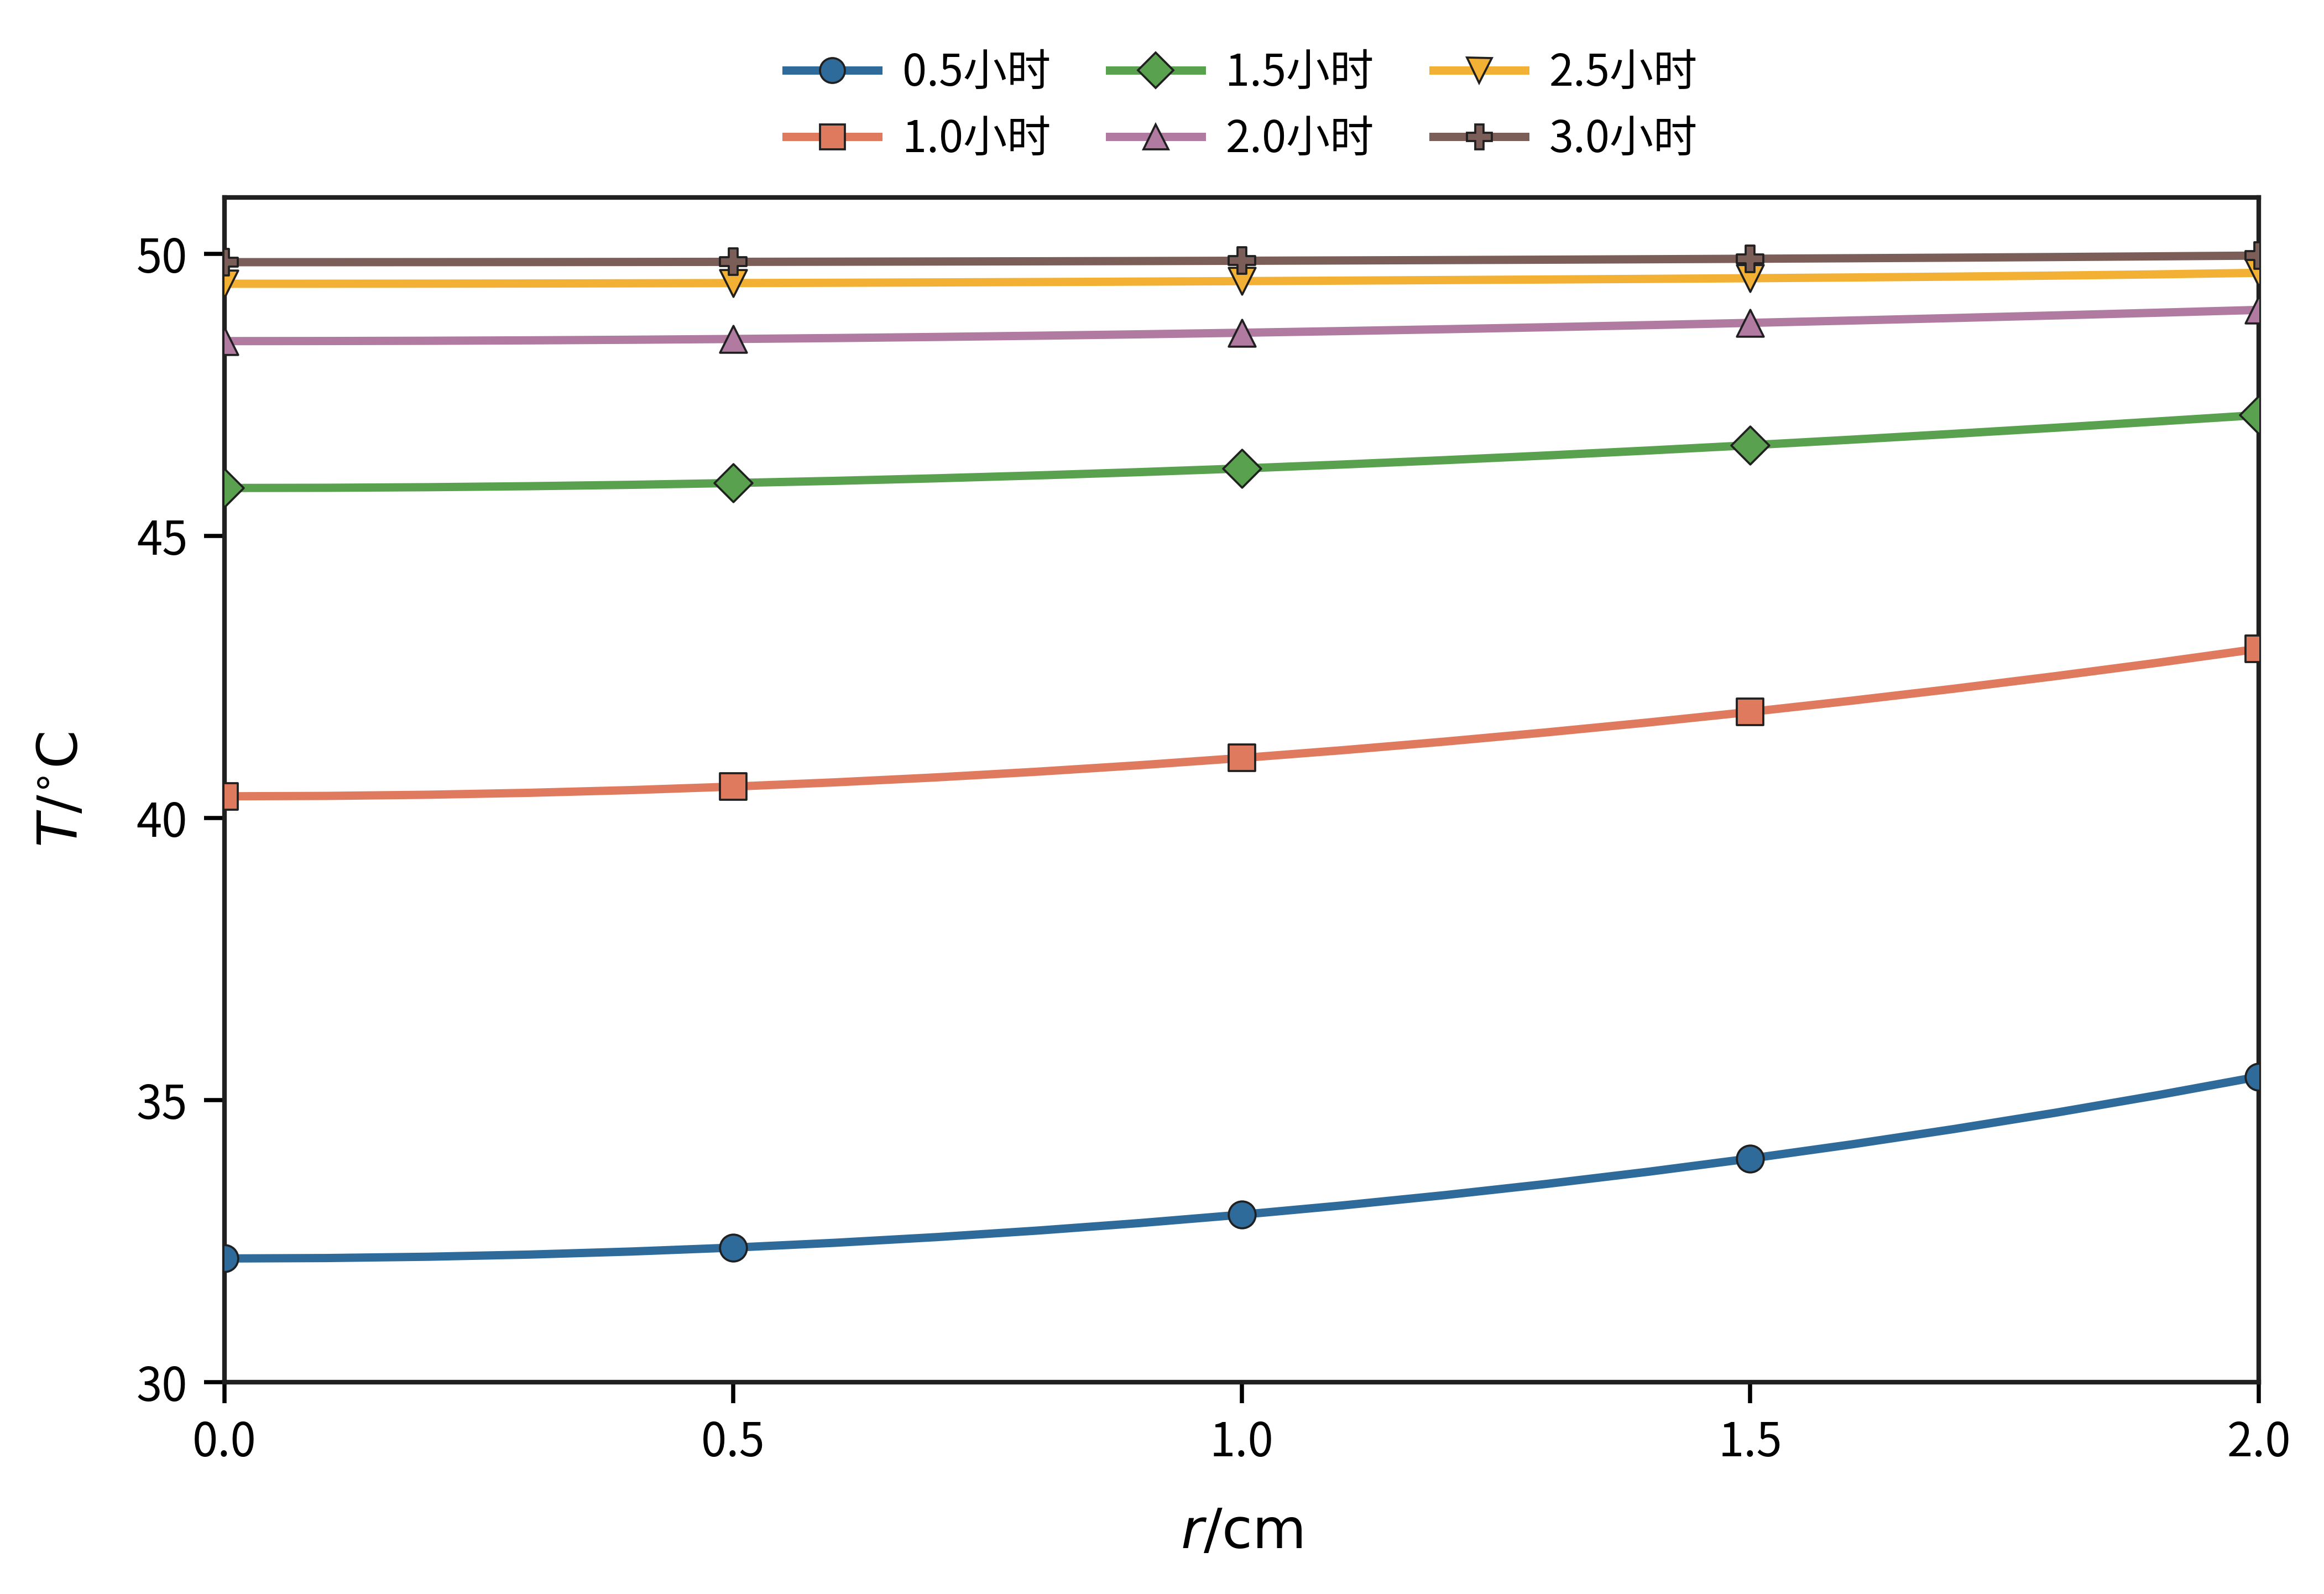
\includegraphics[width=\linewidth]{figures/问题二温度.png}
\caption{温度变化折线图}
\label{fig:q2-temperature-curves}
\end{subfigure}
\hfill
\begin{subfigure}[b]{0.48\textwidth}
\centering
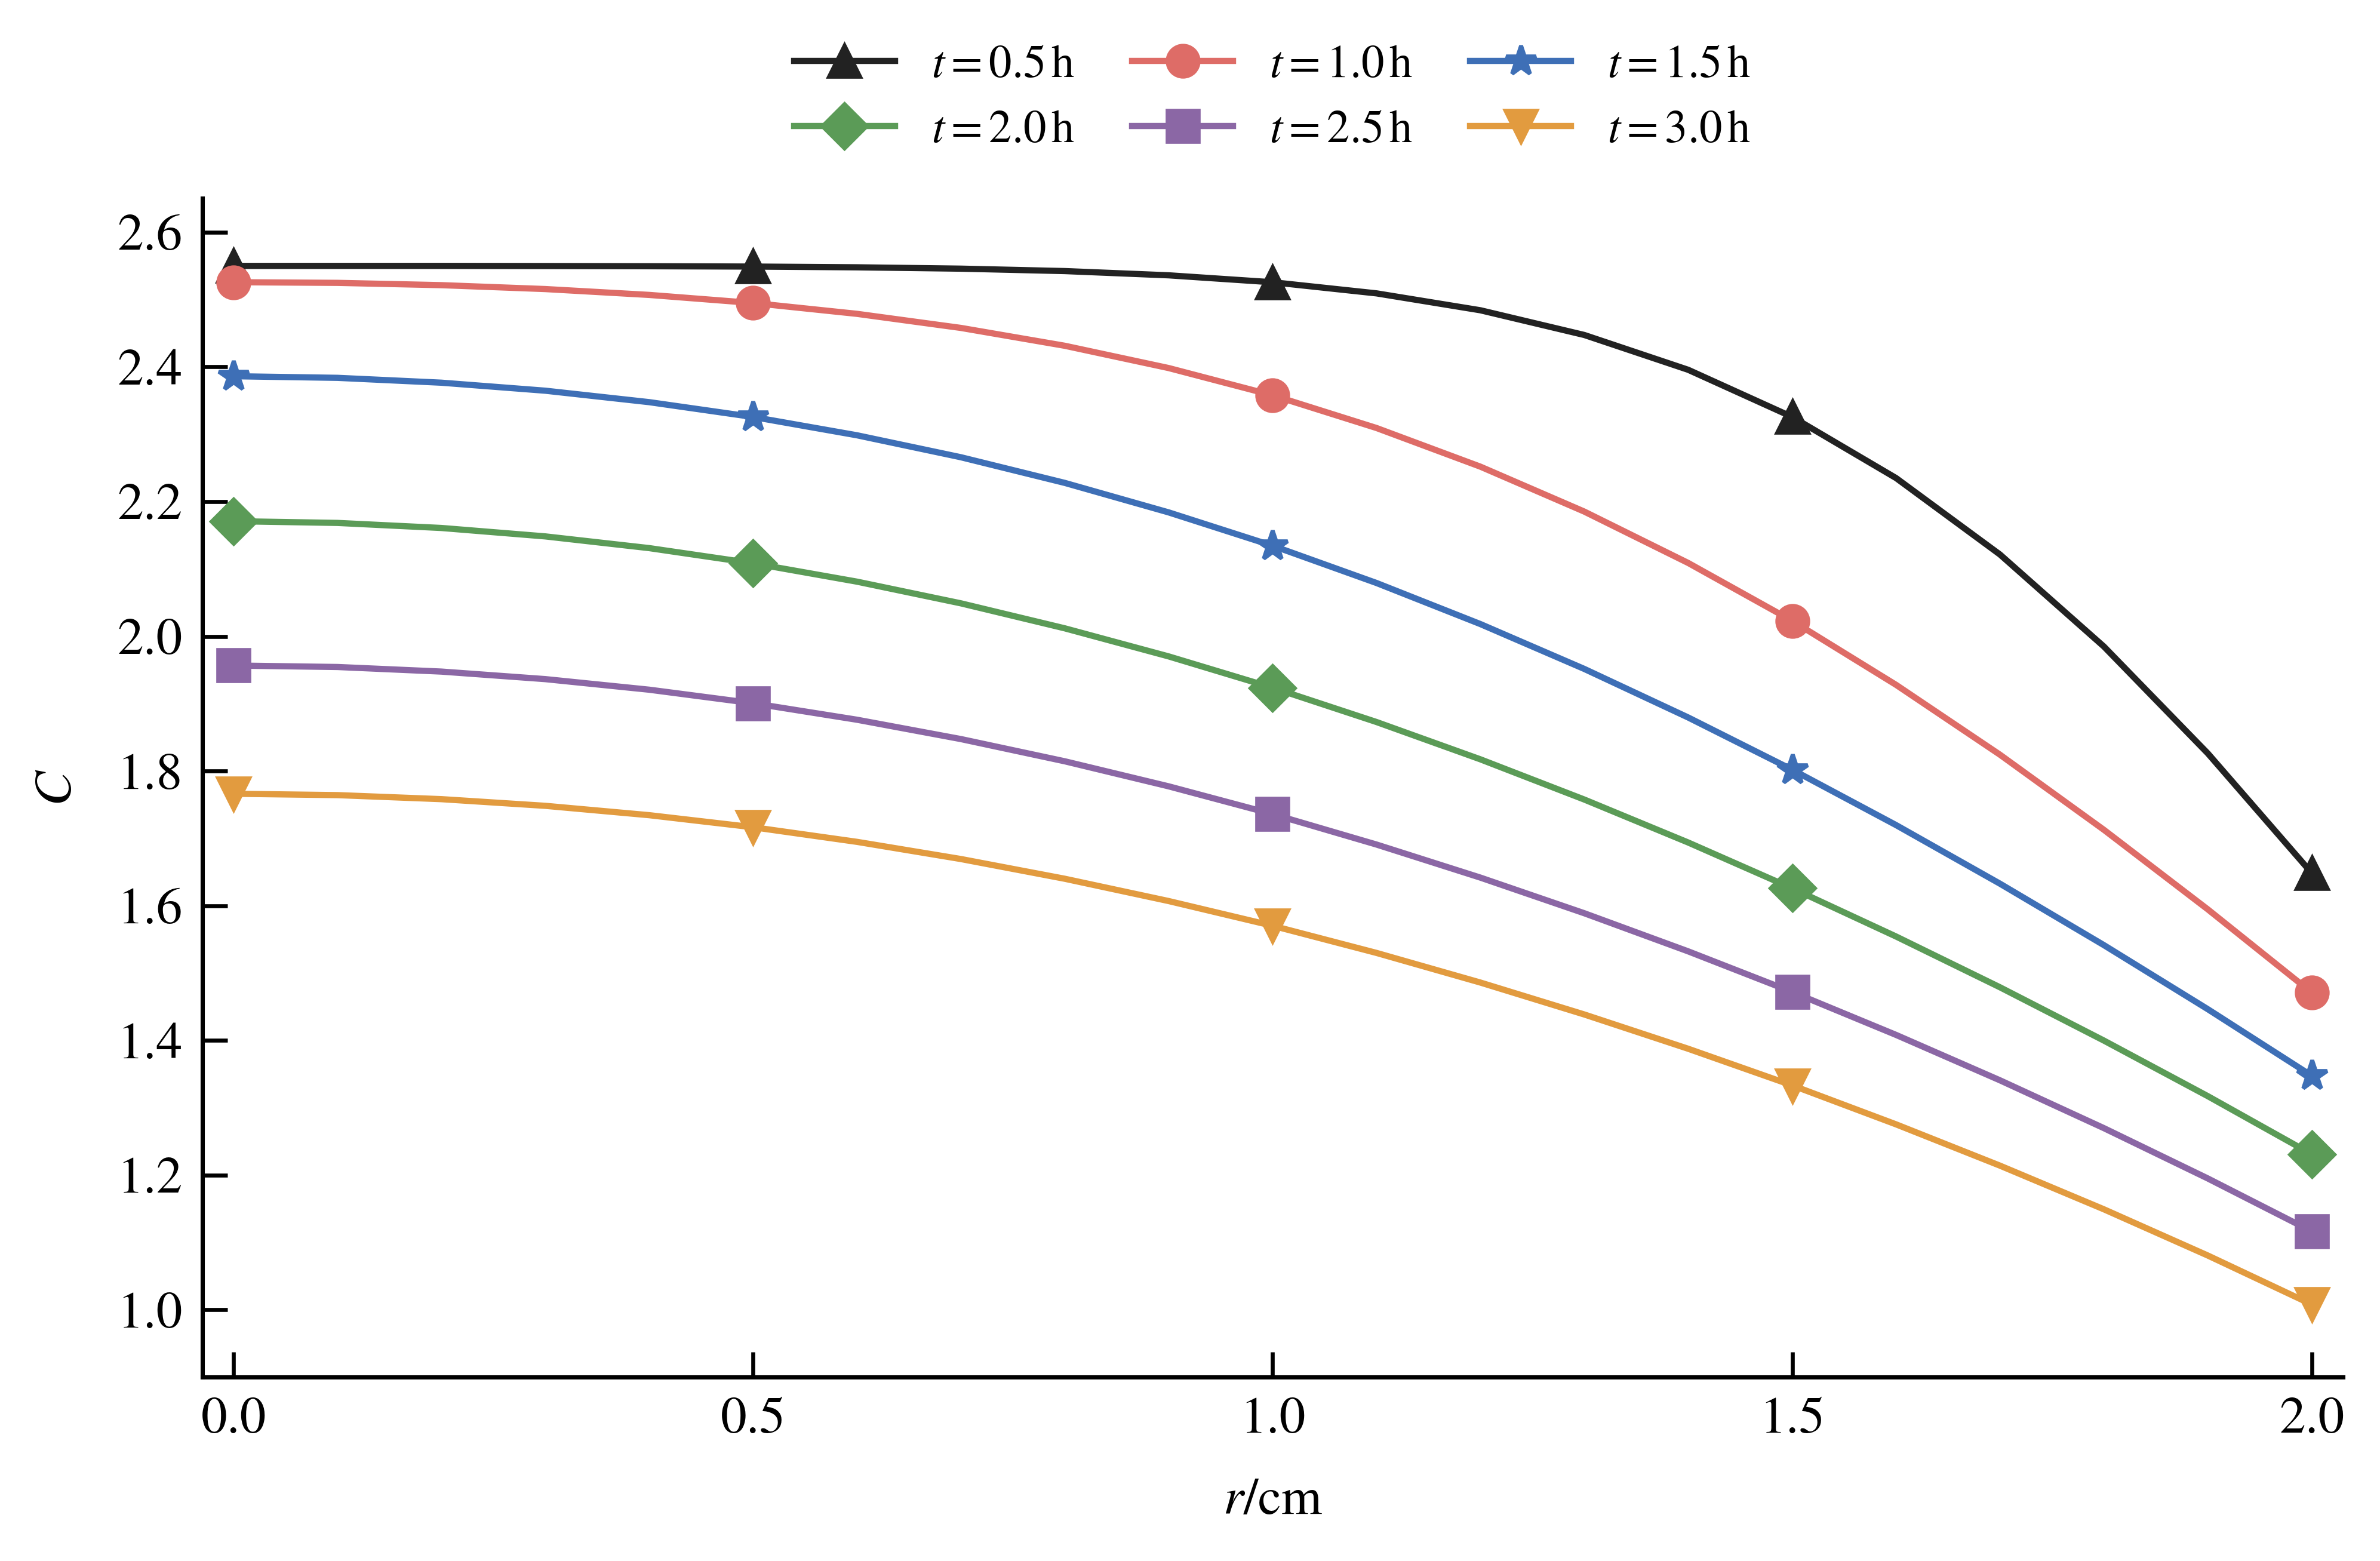
\includegraphics[width=\linewidth]{figures/问题二水分浓度.png}
\caption{水分浓度变化折线图}
\label{fig:q2-moisture-curves}
\end{subfigure}
\caption{问题二模型计算结果}
\label{fig:q2-results}
\end{figure}

\setcounter{table}{2}
\begin{table}[H]
\centering
\renewcommand{\arraystretch}{1.25}
\caption{3小时内药材的温度}
\label{tab:q2-temperature}
\begin{tabularx}{0.9\textwidth}{|>{\centering\arraybackslash}p{0.20\textwidth}|>{\centering\arraybackslash}X|>{\centering\arraybackslash}X|>{\centering\arraybackslash}X|>{\centering\arraybackslash}X|>{\centering\arraybackslash}X|}
\hline
\multirow{2}{*}{时间/h} & \multicolumn{5}{c|}{到药材中心的距离/cm} \\
\cline{2-6}
& 0 & 0.5 & 1 & 1.5 & 2 \\
\hline
0.5 & 32.1892 & 32.3821 & 32.9659 & 33.9608 & 35.4130 \\
\hline
1.0 & 40.3816 & 40.5536 & 41.0605 & 41.8782 & 42.9976 \\
\hline
1.5 & 45.8468 & 45.9348 & 46.1930 & 46.6051 & 47.1401 \\
\hline
2.0 & 48.4502 & 48.4881 & 48.5984 & 48.7736 & 49.0033 \\
\hline
2.5 & 49.4670 & 49.4792 & 49.5136 & 49.5653 & 49.6609 \\
\hline
3.0 & 49.8495 & 49.8553 & 49.8746 & 49.9101 & 49.9664 \\
\hline
\end{tabularx}
\end{table}

\begin{table}[H]
\centering
\renewcommand{\arraystretch}{1.25}
\caption{3小时内药材的水分浓度}
\label{tab:q2-moisture}
\begin{tabularx}{0.9\textwidth}{|>{\centering\arraybackslash}p{0.20\textwidth}|>{\centering\arraybackslash}X|>{\centering\arraybackslash}X|>{\centering\arraybackslash}X|>{\centering\arraybackslash}X|>{\centering\arraybackslash}X|}
\hline
\multirow{2}{*}{时间/h} & \multicolumn{5}{c|}{到药材中心的距离/cm} \\
\cline{2-6}
& 0 & 0.5 & 1 & 1.5 & 2 \\
\hline
0.5 & 2.5499 & 2.5489 & 2.5256 & 2.3257 & 1.6486 \\
\hline
1.0 & 2.5257 & 2.4948 & 2.3578 & 2.0230 & 1.4711 \\
\hline
1.5 & 2.3861 & 2.3256 & 2.1344 & 1.8020 & 1.3476 \\
\hline
2.0 & 2.1709 & 2.1084 & 1.9236 & 1.6259 & 1.2311 \\
\hline
2.5 & 1.9566 & 1.9006 & 1.7360 & 1.4720 & 1.1166 \\
\hline
3.0 & 1.7662 & 1.7165 & 1.5702 & 1.3333 & 1.0081 \\
\hline
\end{tabularx}
\end{table}

\subsection{问题三模型的建立与求解}

\subsubsection{第二问模型的继承与长期边界闭合}

问题三不再改变药材的几何尺寸和物性关系，而是在问题二模型的基础上延长计算时间，直至药材全域含水率满足干燥要求。因此，本问仍采用固定半径$R=0.02\,\mathrm{m}$的一维径向模型，温度场和含水率场分别满足式\eqref{eq:q2-variable-heat}和式\eqref{eq:q2-variable-moisture}，密度、比热容、导热系数和扩散系数均沿用式\eqref{eq:q2-variable-properties}。

附件1给出的烘房环境数据覆盖$0\le t\le t_a=14400\,\mathrm{s}$，采样间隔为$60\,\mathrm{s}$。在该区间内保留全部测量点，并按问题一的方法作分段线性插值。第三问的计算时间远大于$4\,\mathrm h$，题面未给出后续环境数据，因此取$3$--$4\,\mathrm h$内全部等间隔样本的算术平均：
\begin{equation}
\overline T_\infty=\frac{1}{N_p}
\sum_{t_j\ge10800\,\mathrm{s}}T_{\infty,j},
\qquad
\overline C_\infty=\frac{1}{N_p}
\sum_{t_j\ge10800\,\mathrm{s}}C_{\infty,j}.
\label{eq:q3-environment-average}
\end{equation}
该区间含首尾端点，共有$N_p=61$个样本。由附件1计算得到
\begin{equation}
\overline T_\infty=49.9989344262\,{}^\circ\mathrm C,
\qquad
\overline C_\infty=0.0499875410\,\mathrm{kg/kg}.
\label{eq:q3-environment-average-value}
\end{equation}
因此，长期环境边界定义为
\begin{equation}
\bigl(T_\infty(t),C_\infty(t)\bigr)=
\begin{cases}
\bigl(T_{\infty,\mathrm{att}}(t),C_{\infty,\mathrm{att}}(t)\bigr),
&0\le t<t_a,\\
\bigl(\overline T_\infty,\overline C_\infty\bigr),
&t\ge t_a.
\end{cases}
\label{eq:q3-environment-extension}
\end{equation}
本文所有第三问主解及辅助算法均采用式\eqref{eq:q3-environment-extension}，保证算法比较使用相同的边界输入。

\subsubsection{烘干结束判据}

题目要求烘干结束条件为药材各处的水分浓度均低于$0.15\,\mathrm{kg/kg}$。定义全域最大含水率
\begin{equation}
C_{\max}(t)
=
\max_{0\le r\le R}C(r,t),
\label{eq:q3-global-maximum}
\end{equation}
并构造事件函数
\begin{equation}
g(t)=C_{\max}(t)-0.15.
\label{eq:q3-event-function}
\end{equation}
连续临界时刻定义为
\begin{equation}
\boxed{
t_*
=
\inf
\left\{
t>0:C_{\max}(t)<0.15
\right\}.
}
\label{eq:q3-drying-time}
\end{equation}
有限体积解采用分段线性空间重构，其单元内最大值必在端点取得，故计算全部节点的最大值即可得到离散重构的全域最大值。计算结果显示，临界阶段的控制位置为圆柱中心$r=0$。

临界时刻是由场变量导出的决策量，需与场误差分开检查。若阈值附近控制最大值的分支光滑且$g'(t_*)\ne0$，对扰动后的零点作一阶展开可得
\begin{equation}
\delta t_*
\approx-\frac{\delta g(t_*)}{g'(t_*)}.
\label{eq:q3-event-sensitivity}
\end{equation}
式\eqref{eq:q3-event-sensitivity}说明，末期下降斜率较小时，较小的含水率偏差也可能转化为可见的时刻偏差；该式只用于解释局部敏感性，不作为严格误差界。

\subsubsection{数值离散与临界时刻求解}

固定半径下取无量纲坐标$\xi=r/R\in[0,1]$。为同时分辨内部缓变区和表层陡峭梯度，主计算使用$N=12160$个径向区间，其中$[0,0.9]$布置$5760$个等距区间，$[0.9,1]$布置$6400$个等距区间，即
\begin{equation}
\xi_j=
\begin{cases}
0.9j/5760, & 0\le j\le5760,\\
0.9+0.1(j-5760)/6400, & 5760<j\le12160.
\end{cases}
\qquad
\begin{aligned}
\Delta r_{\mathrm{in}}&=3.125\,\mu\mathrm m,\\
\Delta r_{\mathrm{surf}}&=0.3125\,\mu\mathrm m.
\end{aligned}
\label{eq:q3-space-grid}
\end{equation}
题目要求的$0.1\,\mathrm{cm}$输出位置均与网格节点对齐。

空间方向沿用式\eqref{eq:q2-fvm-interior}--\eqref{eq:q2-fvm-surface}的守恒有限体积格式；界面导热系数与扩散系数采用正值调和平均
\begin{equation}
a_{i+\frac12}
=\frac{2a_i a_{i+1}}{a_i+a_{i+1}},
\qquad a\in\{k,D\},
\label{eq:q3-face-harmonic}
\end{equation}
从而以单一导通系数计算同一控制面的守恒通量，并保持系数为正。

时间方向首步采用后向 Euler，随后采用可变步长 BDF2\cite{hairer1996}。记当前步长$h_n=t_{n+1}-t_n$、步长比$q=h_n/h_{n-1}$，则
\begin{equation}
\left.\frac{\partial\phi}{\partial t}\right|_{t_{n+1}}
\approx\frac{1}{h_n}
\left[
\frac{1+2q}{1+q}\phi^{n+1}
-(1+q)\phi^n
+\frac{q^2}{1+q}\phi^{n-1}
\right].
\label{eq:q3-bdf2}
\end{equation}
主时间计划在首分钟取$h=0.0078125\,\mathrm s$，随后以不超过$2$倍的比例逐级放宽，在附件数据及其$60\,\mathrm s$过渡段内最终取$h=0.125\,\mathrm s$，长期阶段最终取$h=1\,\mathrm s$。全部步长均整除$60\,\mathrm s$，因而外界数据折点和结果输出点均为时间节点。

温度和含水率在每个时间层内联合 Picard 迭代。第$m$次迭代由候选含水率更新$\rho,c_p,k$，求得温度后再更新$D(C,T_K)$并求含水率。更新量须满足
\begin{equation}
\left\|\Delta T^{(m+1)}-\Delta T^{(m)}\right\|_\infty
<2\times10^{-12},
\qquad
\left\|\Delta C^{(m+1)}-\Delta C^{(m)}\right\|_\infty
<2\times10^{-13}.
\label{eq:q3-picard-criterion}
\end{equation}
达到更新量阈值后，程序用最终候选状态重新计算全部物性和通量，并逐控制体核验离散平衡残差；相对残差阈值取$10^{-10}$，另显式计入双精度舍入容差。只有更新量与残差两项均通过时才接受该时间步。

当相邻时间层满足$g(t_n)\ge0$且$g(t_{n+1})<0$时，对最近三个时间层的每个节点构造二次时间插值多项式$P_i(t)$，并定义离散事件函数
\begin{equation}
g_h(t)=\max_{0\le i\le N}P_i(t)-0.15.
\label{eq:q3-discrete-event}
\end{equation}
在末个时间步内对$g_h$作二分搜索，直至严格下穿区间$[t_{h,-},t_{h,+}]$满足
\begin{equation}
g_h(t_{h,-})\ge0,
\qquad
g_h(t_{h,+})<0,
\qquad
t_{h,+}-t_{h,-}<10^{-4}\,\mathrm s.
\label{eq:q3-event-bracket}
\end{equation}
该宽度只是所选离散解的求根分辨率，不等于偏微分方程离散误差。每个 Picard 子步产生温度、含水率各一个三对角方程组，均用 Thomas 算法求解；网格几何量和工作数组的复用只影响效率，不改变数值格式。

% 配图建议：在此处或下一小节开头插入“问题三各径向位置含水率随时间变化曲线”。
% 横轴为时间/h，纵轴为含水率/(kg/kg)，绘制r=0,0.5,1.0,1.5,2.0 cm五条曲线，
% 并添加C=0.15水平阈值线和t=57.4723 h竖直事件线。

\subsubsection{模型计算结果}

主计算共接受$320842$个隐式时间步。严格下穿区间为
\begin{equation}
\boxed{
t_{h,-}=206900.236572266\,\mathrm s,
\qquad
t_{h,+}=206900.236633301\,\mathrm s.
}
\label{eq:q3-final-time}
\end{equation}
在$t_{h,+}$处，全网格未舍入最大含水率为$0.149999999991\,\mathrm{kg/kg}$，控制节点为圆心，圆心下降斜率为$-2.912878\times10^{-7}\,\mathrm{kg/(kg\,s)}$。下文空间、时间和事件定位给出的临界时刻综合经验误差估计为$\widehat\varepsilon_t=0.035503\,\mathrm s$，故向上保留四位小数的工艺报告值取
\begin{equation}
\boxed{
t_{\mathrm{rep}}
=10^{-4}\left\lceil
10^4\frac{t_{h,+}+\widehat\varepsilon_t}{3600}
\right\rceil
=57.4723\,\mathrm h.
}
\label{eq:q3-reported-time}
\end{equation}
该取值在当前模型和经验误差估计下留有约$7.86\times10^{-3}\,\mathrm s$的舍入余量。典型时刻的径向含水率见表\ref{tab:q3-moisture}。

\begin{table}[H]
\centering
\renewcommand{\arraystretch}{1.2}
\caption{药材烘干过程的水分浓度}
\label{tab:q3-moisture}
\begin{tabularx}{0.9\textwidth}{|>{\centering\arraybackslash}p{0.20\textwidth}|>{\centering\arraybackslash}X|>{\centering\arraybackslash}X|>{\centering\arraybackslash}X|>{\centering\arraybackslash}X|>{\centering\arraybackslash}X|}
\hline
\multirow{2}{*}{时间/h} & \multicolumn{5}{c|}{到药材中心的距离/cm} \\
\cline{2-6}
& 0 & 0.5 & 1.0 & 1.5 & 2.0 \\
\hline
6 & 1.0170 & 0.9881 & 0.9015 & 0.7550 & 0.5328 \\
\hline
12 & 0.4561 & 0.4432 & 0.4031 & 0.3297 & 0.1642 \\
\hline
18 & 0.2988 & 0.2915 & 0.2687 & 0.2253 & 0.0845 \\
\hline
24 & 0.2378 & 0.2327 & 0.2167 & 0.1855 & 0.0665 \\
\hline
30 & 0.2058 & 0.2018 & 0.1892 & 0.1641 & 0.0598 \\
\hline
36 & 0.1859 & 0.1825 & 0.1718 & 0.1504 & 0.0566 \\
\hline
42 & 0.1721 & 0.1691 & 0.1597 & 0.1407 & 0.0549 \\
\hline
48 & 0.1618 & 0.1592 & 0.1507 & 0.1334 & 0.0537 \\
\hline
54 & 0.1539 & 0.1514 & 0.1436 & 0.1277 & 0.0530 \\
\hline
57.4723 & 0.1500 & 0.1477 & 0.1402 & 0.1249 & 0.0527 \\
\hline
\end{tabularx}
\end{table}

由表\ref{tab:q3-moisture}可见，任一时刻的含水率均由中心向表面递减，表明水分从内部持续向表面迁移。表面含水率较早接近环境水平，而中心含水率下降最慢，故最终烘干时长由中心位置控制。末行中心值显示为$0.1500$是四位小数舍入结果，事件判断使用的是未舍入双精度数值。

% 配图建议：表5之后插入“问题三不同时刻径向含水率剖面图”。
% 建议选取t=6,12,24,36,48 h和t=t_*，横轴r/cm、纵轴C/(kg/kg)，
% 用不同线型而非仅用颜色区分，以保证黑白打印可读。
%
% 可选配图：绘制时间--半径含水率热图，横轴t/h、纵轴r/cm、色标为C/(kg/kg)；
% 不建议采用三维曲面作为唯一主图，因为三维透视会遮挡中心和表面的小幅差异。

\subsubsection{主方法的空间--时间收敛性}

主方法的空间检验固定时间计划，采用$N=3040,6080,12160$三层相似加密网格；时间检验固定$N=12160$，将“初始/附件期/长期”三段最大步长分别取为$(0.03125,0.5,4)$、$(0.015625,0.25,2)$和$(0.0078125,0.125,1)\,\mathrm s$。全部场差异在$60\,\mathrm s$至$206880\,\mathrm s$的共同输出时段、281个共同随体位置上计算，临界时刻则单独比较。

对三级结果$Q_h,Q_{h/2},Q_{h/4}$，观测阶与带$1.5$安全系数的细解余量估计定义为\cite{roache1998}
\begin{equation}
p_{\mathrm{obs}}
=\log_2\frac{|Q_h-Q_{h/2}|}{|Q_{h/2}-Q_{h/4}|},
\qquad
\widehat\varepsilon_Q
=1.5\frac{|Q_{h/2}-Q_{h/4}|}{2^{p_{\mathrm{obs}}}-1}.
\label{eq:q3-richardson-estimate}
\end{equation}
实际三级差值见表\ref{tab:q3-convergence}。

\begin{table}[H]
\centering
\small
\renewcommand{\arraystretch}{1.15}
\caption{第三问主方法的独立空间、时间加密结果}
\label{tab:q3-convergence}
\begin{tabularx}{\textwidth}{>{\raggedright\arraybackslash}p{0.17\textwidth} >{\centering\arraybackslash}X >{\centering\arraybackslash}X >{\centering\arraybackslash}p{0.12\textwidth} >{\centering\arraybackslash}X}
\hline
指标与加密方向 & 粗--中差异 & 中--细差异 & $p_{\mathrm{obs}}$ & 细解余量估计\\
\hline
$T$，空间 & $1.42505\times10^{-7}\,{}^\circ\mathrm C$ & $3.56262\times10^{-8}\,{}^\circ\mathrm C$ & $2.000001$ & $1.78131\times10^{-8}\,{}^\circ\mathrm C$\\
$T$，时间 & $5.19787\times10^{-7}\,{}^\circ\mathrm C$ & $1.29712\times10^{-7}\,{}^\circ\mathrm C$ & $2.002610$ & $6.48559\times10^{-8}\,{}^\circ\mathrm C$\\
$C$，空间 & $5.17710\times10^{-6}$ & $1.29271\times10^{-6}$ & $2.001742$ & $6.46356\times10^{-7}$\\
$C$，时间 & $4.12778\times10^{-8}$ & $1.03212\times10^{-8}$ & $1.999759$ & $5.16174\times10^{-9}$\\
$t_*$，空间 & $0.282288\,\mathrm s$ & $0.0705566\,\mathrm s$ & $2.000312$ & $0.0352783\,\mathrm s$\\
$t_*$，时间 & $1.15967\times10^{-3}\,\mathrm s$ & $3.05176\times10^{-4}\,\mathrm s$ & $1.925999$ & $1.63487\times10^{-4}\,\mathrm s$\\
\hline
\end{tabularx}
\end{table}

空间和时间加密均呈接近二阶的响应。将空间、时间估计相加，得到温度和含水率在上述共同采样集上的综合经验误差估计
\begin{equation}
\widehat\varepsilon_T=8.26690\times10^{-8}\,{}^\circ\mathrm C,
\qquad
\widehat\varepsilon_C=6.51518\times10^{-7}\,\mathrm{kg/kg}.
\label{eq:q3-field-error-estimates}
\end{equation}
临界时刻再计入$6.10352\times10^{-5}\,\mathrm s$的事件区间宽度，得到
\begin{equation}
\widehat\varepsilon_t
=0.0352783+0.000163487+0.0000610352
=0.035503\,\mathrm s.
\label{eq:q3-time-error-estimate}
\end{equation}
这些量依赖式\eqref{eq:q3-richardson-estimate}的渐近展开假设，是保守的工程误差估计而非严格数学上界。主解全部时间步均通过最终状态残差检查，最大热量、水分离散平衡相对残差分别为$1.52\times10^{-11}$和$2.03\times10^{-14}$；这些残差只验证所选离散方程的收支，不代表完整热力学模型已经得到实验验证。

\subsubsection{同一径向模型的跨算法一致性}

三级自收敛回答“同一有限体积离散继续加密时结果如何变化”，但不能排除各级网格共同继承的实现偏差。为此，本文采用分区 Chebyshev--Lobatto 弱形式谱元\cite{trefethen2000}和五阶 Radau IIA 方法\cite{hairer1996}重新求解相同的径向初边值问题。谱元使用$s=(r/R)^2$坐标、9个径向子区间；最高阶算例每区采用64阶多项式，共577个场自由度。它在空间近似、边界施加、时间推进以及空间最大值搜索方面均不同于有限体积主方法。

谱元的24、40、64阶加密中，含水率最大采样差由$1.93020\times10^{-7}$降至$2.67740\times10^{-8}\,\mathrm{kg/kg}$，相邻临界时刻差分别为$1.70841\times10^{-5}\,\mathrm s$和$1.01806\times10^{-5}\,\mathrm s$；在64阶空间离散上收紧 Radau 容差后，含水率最大采样差为$1.51519\times10^{-11}\,\mathrm{kg/kg}$，临界时刻差为$3.10441\times10^{-5}\,\mathrm s$。这些是共同采样集上的观测差异，不是严格误差界。

本文进一步从保存的全精度结果中，对有限体积与64阶谱元在3448个公共分钟、题目要求的21个实际径向位置上重新计算差异，得到
\begin{equation}
\begin{aligned}
E_T^{\mathrm{FVM,SEM}}&=4.57080\times10^{-8}\,{}^\circ\mathrm C,\\
E_C^{\mathrm{FVM,SEM}}&=4.67183\times10^{-8}\,\mathrm{kg/kg},\\
E_t^{\mathrm{FVM,SEM}}&=0.0233898\,\mathrm s.
\end{aligned}
\label{eq:q3-cross-algorithm-differences}
\end{equation}
谱元临界时刻为$206900.213243\,\mathrm s$，与有限体积结果的差异小于式\eqref{eq:q3-time-error-estimate}的经验估计。由此可认为，第三问的径向场分布及四位小数时长没有表现出明显的单一空间离散或时间推进依赖；这一结论仍只属于共同模型下的数值交叉证据，不能替代物理实验验证。

综上，有限体积自收敛和谱元同模型复算分别检验数值稳定性与跨离散一致性。第三问正式报告$t_{\mathrm{rep}}=57.4723\,\mathrm h$；该数字在给定物性、传递系数和长期边界闭合下具有稳定的数值依据，但不包含这些建模假设本身的不确定性。

% 第三问实验依据（相对于项目根目录）：
% problem3/q3_3algo/home/zyf/CUMCM/q3/problem3_fine/validation_report.md
% problem3/q3_3algo/home/zyf/CUMCM/q3/q3q4more/experiments_spectral/Q3/comparison_report.json

\subsection{问题四模型的建立与求解}

\subsubsection{数据相容性与模型选择}
\label{sec:q4-compatibility}

问题四同时给出半径时序和密度经验式，二者能否共同描述同一守恒材料，需要先作相容性检验。以下暂将附录4的$\rho_w(C)=760+90C$解释为精确的局部湿体积密度，其体积基准与圆柱几何体积一致。由干基含水率定义$C=\mathrm dm_w/\mathrm dm_d$，局部干固体体积密度及其上界为
\begin{equation}
\rho_d(C)=\frac{\rho_w(C)}{1+C}
=\frac{760+90C}{1+C}\le760\,\mathrm{kg/m^3},
\qquad C\ge0.
\label{eq:q4-true-dry-density-bound}
\end{equation}
初始温湿状态均匀，故初始总干质量为
\begin{equation}
\rho_{d0}=\frac{760+90C_0}{1+C_0}=278.7323944\,\mathrm{kg/m^3},
\qquad
M_{d0}=\pi R_0^2L_0\rho_{d0}=0.08756636\,\mathrm{kg}.
\label{eq:q4-initial-dry-mass}
\end{equation}
若干质量守恒，且当前圆柱长度$L(t)\le L_0=0.25\,\mathrm m$，则不论内部含水率如何分布、材料层如何变形，都有
\begin{equation}
\begin{aligned}
M_{d0}&=\int_{\text{药材体积}}\rho_d\,\mathrm dV
\le760\pi R(t)^2L(t)\le760\pi R(t)^2L_0,\\
R(t)&\ge R_0\sqrt{\frac{\rho_{d0}}{760}}
=1.211203\,\mathrm{cm}.
\end{aligned}
\label{eq:q4-absolute-radius-bound}
\end{equation}
附件2在$24\,\mathrm h$的半径已为$1.204\,\mathrm{cm}$，在$72\,\mathrm h$进一步降至$1.198\,\mathrm{cm}$，均低于式\eqref{eq:q4-absolute-radius-bound}。这一必要条件仅由题给附录4、初始条件、圆柱体积和质量定义推得，并未使用仿射假设或扩散方程。因而，\textbf{精确局部湿体积密度、实测外半径、干质量守恒及长度不增加，在当前圆柱解释下不能全部成立}；仅改变径向映射或增加端面交换不能消除该矛盾。若保留前三项，$72\,\mathrm h$的长度即使在完全无水的极限下也须不小于$25.5541\,\mathrm{cm}$。

为给出利用附件2的工程基线，本文保留实测半径，采用固定长度的径向仿射运动，并将附录4密度限定为温度方程中的有效显热储存参数，记作$\rho_{\mathrm{eff}}(C)$。这保留了附录经验式在热方程中的数值形式，但放松了它作为精确局部湿体积密度的解释；不再要求$\rho_{\mathrm{eff}}=(1+C)\rho_d$。下文的烘干时长在该闭合假设下成立，真实密度解释下的守恒对照见本问末尾。

\subsubsection{收缩假设与半径插值}

问题四将问题三的固定区域长期干燥推广到半径随时间变化的收缩区域，并在全部计算时段采用题面附录4给出的物性关系。时刻$t$的药材区域为
\begin{equation}
\Omega(t)=\{r:0\le r\le R(t)\},
\label{eq:q4-moving-domain}
\end{equation}
其中$R(t)$由附件2确定。基于前述模型选择，假设药材保持轴对称圆柱形，长度固定为$L_0$，各材料层作径向均匀仿射运动；$C$表示随干物质运动的干基含水率，收缩本身不产生额外水分源项。为与前文公式一致，下文热方程中的$\rho(C)$均指$\rho_{\mathrm{eff}}(C)$。固定长度是缺少轴向观测时采用的基线假设，并非由附件2推出。

附件2包含$145$个测点，时间范围为$0\le t\le259200\,\mathrm s$，半径从$R_0=2.000\,\mathrm{cm}$减小至$1.198\,\mathrm{cm}$。测点之间采用分段线性插值：
\begin{equation}
R(t)
=R_j+
\frac{t-t_j}{t_{j+1}-t_j}
\left(R_{j+1}-R_j\right),
\qquad t_j\le t\le t_{j+1}.
\label{eq:q4-radius-interpolation}
\end{equation}
若计算超过$72\,\mathrm h$，则令$R(t)=1.198\,\mathrm{cm}$；但本问所得结束时刻早于$72\,\mathrm h$，该延拓不参与最终结果。

\subsubsection{材料坐标与移动区域方程}

取初始时位于相对位置$\xi$的材料层在时刻$t$仍位于$r=\xi R(t)$，即
\begin{equation}
\boxed{
\xi=\frac{r}{R(t)},
\qquad 0\le\xi\le1.
}
\label{eq:q4-material-coordinate}
\end{equation}
相应的材料骨架径向速度为
\begin{equation}
u_r(r,t)
=\frac{\mathrm dr}{\mathrm dt}
=\frac{\dot R(t)}{R(t)}r.
\label{eq:q4-solid-velocity}
\end{equation}
对随材料运动的任意场$f(r,t)$，材料导数为
\begin{equation}
\frac{\mathrm Df}{\mathrm Dt}
=\left.\frac{\partial f}{\partial t}\right|_r
+u_r\frac{\partial f}{\partial r}.
\label{eq:q4-material-derivative}
\end{equation}
因此，移动物理区域上的传热、传质方程写为
\begin{equation}
\rho(C)c_p(C)\frac{\mathrm DT}{\mathrm Dt}
=\frac{1}{r}\frac{\partial}{\partial r}
\left[rk(C)\frac{\partial T}{\partial r}\right],
\label{eq:q4-physical-heat}
\end{equation}
\begin{equation}
\frac{\mathrm DC}{\mathrm Dt}
=\frac{1}{r}\frac{\partial}{\partial r}
\left[rD(C,T_K)\frac{\partial C}{\partial r}\right].
\label{eq:q4-physical-moisture}
\end{equation}
式\eqref{eq:q4-physical-moisture}以干基含水率为状态量；在均匀仿射收缩假设下，各材料层的参考干质量不变，故几何收缩通过材料运动和时变尺度进入方程，而不另设“浓缩项”。

定义固定区域上的未知量
\begin{equation}
\Theta(\xi,t)=T\bigl(\xi R(t),t\bigr),
\qquad
W(\xi,t)=C\bigl(\xi R(t),t\bigr).
\label{eq:q4-transformed-fields}
\end{equation}
在固定物理坐标$r$下，由链式法则有
\begin{equation}
\left.\frac{\partial f}{\partial t}\right|_r
=\left.\frac{\partial\widehat f}{\partial t}\right|_\xi
-\frac{\dot R}{R}\xi
\frac{\partial\widehat f}{\partial\xi},
\qquad
u_r\frac{\partial f}{\partial r}
=\frac{\dot R}{R}\xi
\frac{\partial\widehat f}{\partial\xi}.
\label{eq:q4-chain-rule}
\end{equation}
两式相加后，网格运动项严格抵消：
\begin{equation}
\boxed{
\frac{\mathrm Df}{\mathrm Dt}
=\left.\frac{\partial\widehat f}{\partial t}\right|_\xi.
}
\label{eq:q4-material-cancellation}
\end{equation}
又因为$\partial/\partial r=R^{-1}\partial/\partial\xi$，圆柱扩散算子满足
\begin{equation}
\frac{1}{r}\frac{\partial}{\partial r}
\left(r\Gamma\frac{\partial f}{\partial r}\right)
=\frac{1}{R(t)^2\xi}
\frac{\partial}{\partial\xi}
\left(\xi\Gamma\frac{\partial\widehat f}{\partial\xi}\right).
\label{eq:q4-radial-operator-transform}
\end{equation}
于是问题四被变换为固定区间$0\le\xi\le1$上的耦合方程
\begin{equation}
\boxed{
\rho(W)c_p(W)\frac{\partial\Theta}{\partial t}
=\frac{1}{R(t)^2\xi}
\frac{\partial}{\partial\xi}
\left[\xi k(W)\frac{\partial\Theta}{\partial\xi}\right],
}
\label{eq:q4-fixed-heat}
\end{equation}
\begin{equation}
\boxed{
\frac{\partial W}{\partial t}
=\frac{1}{R(t)^2\xi}
\frac{\partial}{\partial\xi}
\left[\xi D(W,\Theta_K)\frac{\partial W}{\partial\xi}\right].
}
\label{eq:q4-fixed-moisture}
\end{equation}
其中$\Theta_K=\Theta+273.15$。因$\xi$已被定义为随固体骨架运动的材料坐标，式\eqref{eq:q4-fixed-heat}和式\eqref{eq:q4-fixed-moisture}中不应再次加入与$\dot R$有关的网格对流项，否则会重复计算收缩运动。半径变化主要通过$R(t)^{-2}$改变内部传递时间尺度。

\subsubsection{物性、初始条件与边界条件}

问题四从$t=0$开始统一采用题面附录4的经验公式：
\begin{equation}
\left\{
\begin{aligned}
\rho(W)&=760+90W,\\
c_p(W)&=1850+2150\frac{W}{W+1},\\
k(W)&=0.12+0.20\frac{W}{W+1},\\
D(W,\Theta_K)
&=4.2\times10^{-4}
\exp\!\left(-\frac{0.30}{W}\right)
\exp\!\left(-\frac{3850}{\Theta_K}\right).
\end{aligned}
\right.
\label{eq:q4-properties}
\end{equation}
其单位依次为$\mathrm{kg/m^3}$、$\mathrm{J/(kg\cdot K)}$、$\mathrm{W/(m\cdot K)}$和$\mathrm{m^2/s}$。扩散系数中的温度必须取绝对温度。环境函数沿用式\eqref{eq:q3-environment-extension}：附件1覆盖范围内作分段线性插值，$4\,\mathrm h$后保持附件1末$1\,\mathrm h$环境测量值的算术平均。

初始条件为
\begin{equation}
\Theta(\xi,0)=28\,{}^\circ\mathrm C,
\qquad
W(\xi,0)=2.55\,\mathrm{kg/kg}.
\label{eq:q4-initial-condition}
\end{equation}
圆心处由轴对称性满足
\begin{equation}
\Theta_\xi(0,t)=0,
\qquad
W_\xi(0,t)=0.
\label{eq:q4-center-boundary}
\end{equation}
物理表面的对流换热、传质条件变换到$\xi=1$后为
\begin{equation}
\frac{k(W_s)}{R(t)}\Theta_\xi(1,t)
=h\left[T_\infty(t)-\Theta_s(t)\right],
\label{eq:q4-surface-heat}
\end{equation}
\begin{equation}
\frac{D(W_s,\Theta_{K,s})}{R(t)}W_\xi(1,t)
=h_m\left[C_\infty(t)-W_s(t)\right],
\label{eq:q4-surface-moisture}
\end{equation}
其中$h=25\,\mathrm{W/(m^2\cdot K)}$、$h_m=8\times10^{-7}\,\mathrm{m/s}$沿用题面前述参数。

\subsubsection{空间离散与自适应隐式求解}

在固定材料区间建立节点型有限体积网格
\begin{equation}
0=\xi_0<\xi_1<\cdots<\xi_N=1.
\label{eq:q4-grid}
\end{equation}
为解析表面附近的陡峭含水率梯度，将$0\le\xi\le0.9$作为内区，将$0.9<\xi\le1$作为表面加密区，后者的步长取内区的$1/10$。正式计算采用$N=6080$，故
\begin{equation}
\Delta\xi_{\mathrm b}
=\frac{0.9+10\times0.1}{6080}
=3.125\times10^{-4},
\qquad
\Delta\xi_{\mathrm s}
=3.125\times10^{-5}.
\label{eq:q4-grid-spacings}
\end{equation}
内区和表面区分别包含$2880$和$3200$个区间。初始半径下两区对应的物理步长分别为$6.25\,\mu\mathrm m$和$0.625\,\mu\mathrm m$，随半径收缩还会同比减小。

令节点控制体边界为$\xi_{i-1/2}$和$\xi_{i+1/2}$，圆柱径向储存权重为
\begin{equation}
M_i
=\int_{\xi_{i-1/2}}^{\xi_{i+1/2}}\xi\,\mathrm d\xi
=\frac{\xi_{i+1/2}^2-\xi_{i-1/2}^2}{2},
\label{eq:q4-storage-weight}
\end{equation}
其中$\xi_{-1/2}=0$、$\xi_{N+1/2}=1$。统一记
\begin{equation}
(\phi,S,\Gamma,b,\phi_\infty)
=
\begin{cases}
(\Theta,\rho c_p,k,h,T_\infty),&\text{温度方程},\\
(W,1,D,h_m,C_\infty),&\text{水分方程}.
\end{cases}
\label{eq:q4-unified-variables}
\end{equation}
界面传递系数采用调和平均
\begin{equation}
\Gamma_{i+1/2}
=\frac{2\Gamma_i\Gamma_{i+1}}
{\Gamma_i+\Gamma_{i+1}},
\label{eq:q4-harmonic-mean}
\end{equation}
内部界面通量写成
\begin{equation}
F_{i+1/2}
=\xi_{i+1/2}\Gamma_{i+1/2}
\frac{\phi_{i+1}-\phi_i}{\xi_{i+1}-\xi_i}.
\label{eq:q4-face-flux}
\end{equation}
对控制方程作体积积分，得到半离散方程
\begin{equation}
S_iM_i\frac{\mathrm d\phi_i}{\mathrm dt}
=\frac{F_{i+1/2}-F_{i-1/2}}{R(t)^2},
\qquad 1\le i\le N-1.
\label{eq:q4-fvm-interior}
\end{equation}
中心和表面通量直接取为
\begin{equation}
F_{-1/2}=0,
\qquad
F_{N+1/2}
=R(t)b\left(\phi_\infty-\phi_N\right),
\label{eq:q4-boundary-fluxes}
\end{equation}
再代入同一通量差公式即可得到$i=0,N$两个边界控制体方程。这样无需在$\xi=0$处直接计算$1/\xi$，内部通量也在相邻控制体之间严格成对抵消。

空间离散后形成$2(N+1)$维刚性非线性常微分方程组，采用自适应阶次的隐式 BDF 方法整体求解温湿耦合状态，并向求解器提供块三对角 Jacobian 稀疏结构。正式计算的相对容差为$5\times10^{-12}$，温度和含水率绝对容差分别为$5\times10^{-12}$和$5\times10^{-14}$；前$4\,\mathrm h$环境变化较快，最大内部步长限制为$0.5\,\mathrm s$，此后取$2.5\,\mathrm s$。每$60\,\mathrm s$保存一次结果，并同步积分表面传质通量以检验全局水分平衡。

第四问输出的是当前物理位置而非固定材料坐标。对任意固定距离$r_q<R(t)$，先计算
\begin{equation}
\xi_q(t)=\frac{r_q}{R(t)},
\qquad
C(r_q,t)=W\bigl(\xi_q(t),t\bigr),
\label{eq:q4-physical-output}
\end{equation}
再由材料网格插值；若$r_q\ge R(t)$，该位置已处于药材外部，Excel 中相应单元格留空。最后一列“药材表面”始终取$W(1,t)$，不能理解为某个固定厘米位置。

\subsubsection{严格干燥判据与安全工艺时长}

定义当前材料区域的最大含水率
\begin{equation}
C_{\max}^{(4)}(t)=\max_{0\le\xi\le1}W(\xi,t),
\label{eq:q4-global-maximum}
\end{equation}
则连续临界时刻为
\begin{equation}
\boxed{
t_*^{(4)}
=\inf\left\{t>0:C_{\max}^{(4)}(t)<0.15\right\}.
}
\label{eq:q4-drying-time}
\end{equation}
程序先在相邻$60\,\mathrm s$输出点之间检出$C_{\max}^{(4)}-0.15$的符号变化，再使用 BDF 稠密输出和 Brent 根求解定位等值点。由于含水率连续且临界点附近严格下降，式\eqref{eq:q4-drying-time}的下确界处仍满足$C_{\max}^{(4)}(t_*^{(4)})=0.15$，任意略晚时刻才满足严格小于。

为了给出可执行的整分钟工艺时长，还需同时计入含水率数值误差的保守估计$\varepsilon_C^{(4)}$和四位小数显示裕量
\begin{equation}
\delta_4=\frac{1}{2}\times10^{-4}=5\times10^{-5}.
\label{eq:q4-display-margin}
\end{equation}
因此定义
\begin{equation}
\boxed{
t_{\mathrm{end}}^{(4)}
=\min\left\{
60n:
C_{\max}^{(4)}(60n)+\varepsilon_C^{(4)}
<0.15-\delta_4,
\ n\in\mathbb N^+
\right\}.
}
\label{eq:q4-safe-end-time}
\end{equation}
在数值误差不超过所取估计量的条件下，该判据保证模型的未舍入含水率严格小于$0.15$；本次计算还使表6保留四位小数后显示为$0.1499$，而非$0.1500$。这里的安全性是给定模型和数值误差估计下的工艺裕量，不是包含模型结构误差的无条件保证。

\subsubsection{模型计算结果}

高精度计算得到连续临界时刻
\begin{equation}
\boxed{
t_*^{(4)}
=183926.094367684\,\mathrm s
=51.0905817688\,\mathrm h.
}
\label{eq:q4-final-crossing}
\end{equation}
取$\varepsilon_C^{(4)}=7.245764\times10^{-7}\,\mathrm{kg/kg}$后，由式\eqref{eq:q4-safe-end-time}得到安全工艺时长
\begin{equation}
\boxed{
t_{\mathrm{end}}^{(4)}
=184080\,\mathrm s
=51.1333333333\,\mathrm h.
}
\label{eq:q4-final-safe-time}
\end{equation}
该时刻全域最大含水率为$0.149921045870\,\mathrm{kg/kg}$。典型时刻的水分浓度和当前半径见表\ref{tab:q4-moisture}。

\begin{table}[H]
\centering
\renewcommand{\arraystretch}{1.18}
\caption{考虑半径收缩时药材烘干过程的水分浓度}
\label{tab:q4-moisture}
\begin{tabularx}{0.94\textwidth}{|>{\centering\arraybackslash}p{0.15\textwidth}|>{\centering\arraybackslash}X|>{\centering\arraybackslash}X|>{\centering\arraybackslash}X|>{\centering\arraybackslash}X|>{\centering\arraybackslash}p{0.16\textwidth}|}
\hline
\multirow{2}{*}{时间/h}
&\multicolumn{4}{c|}{到药材中心的距离/cm}
&\multirow{2}{*}{当前半径/cm}\\
\cline{2-5}
&0&0.5&1.0&药材表面&\\
\hline
6&1.7196&1.5377&1.0226&0.4207&1.3740\\
\hline
12&0.7377&0.6546&0.4083&0.1670&1.2480\\
\hline
18&0.4087&0.3686&0.2397&0.0892&1.2140\\
\hline
24&0.2851&0.2611&0.1790&0.0673&1.2040\\
\hline
30&0.2263&0.2094&0.1493&0.0595&1.2010\\
\hline
36&0.1928&0.1797&0.1317&0.0560&1.2000\\
\hline
42&0.1712&0.1604&0.1200&0.0541&1.2000\\
\hline
48&0.1561&0.1468&0.1116&0.0530&1.2000\\
\hline
51.1333&0.1499&0.1412&0.1080&0.0526&1.2000\\
\hline
\end{tabularx}
\end{table}

表\ref{tab:q4-moisture}表明，收缩过程中最大含水率始终位于中心，移动表面的含水率则最先接近环境水平。与问题三的固定半径、附录3物性模型相比，问题四的连续时长缩短约$6.3817\,\mathrm h$；但这一差异同时包含半径收缩和附录4物性变化，不能全部归因于几何收缩。收缩本身通过式\eqref{eq:q4-fixed-moisture}中的$R(t)^{-2}$因子缩短后期的内部扩散尺度。

\subsubsection{数值检验}

空间收敛检验采用$N=1520,3040,6080$三层相似加密网格。前两层与后两层最大含水率场差分别为$6.945758\times10^{-6}$和$1.736444\times10^{-6}\,\mathrm{kg/kg}$，因而观测阶为
\begin{equation}
p_r
=\frac{\ln\!\left(6.945758\times10^{-6}/1.736444\times10^{-6}\right)}{\ln2}
=1.999997.
\label{eq:q4-spatial-order}
\end{equation}
在观测到的二阶渐近收敛假设下，采用$1.25$倍 Richardson 安全系数得到细网格空间误差的保守估计$7.235205\times10^{-7}\,\mathrm{kg/kg}$；合并时间积分差异后，即得式\eqref{eq:q4-safe-end-time}所用的$\varepsilon_C^{(4)}=7.245764\times10^{-7}\,\mathrm{kg/kg}$。该量是网格收敛证据支持的工程误差估计，并非经严格后验分析证明的误差上界。三层网格的连续临界时刻分别为$183926.492296$、$183926.173952$和$183926.094368\,\mathrm s$。

在$N=6080$网格上进一步收紧 BDF 容差和最大步长，全部公共输出点的最大含水率差为$5.733953\times10^{-10}\,\mathrm{kg/kg}$，连续临界时刻差仅$5.474110\times10^{-6}\,\mathrm s$。通过辅助状态同步积分边界传质通量后，归一化水分库存的最大守恒绝对残差为$1.598721\times10^{-14}$；所有输出时刻的最大含水率均位于中心。这些结果共同表明，空间离散、时间积分、事件定位和整体守恒均已达到支持表6的精度。

\subsubsection{守恒对照与模型结构讨论}
\label{sec:q4-conservation-comparison}

主模型中，干固体守恒由材料映射单独约束。初始干固体分布均匀时，仿射映射的体积Jacobian及骨架干密度满足
\begin{equation}
J(t)=\left[\frac{R(t)}{R_0}\right]^2,
\qquad
\rho_d^{\mathrm{sk}}(t)J(t)=\rho_{d0}^{\mathrm{sk}},
\qquad
M_d^{\mathrm{sk}}=\pi L_0R(t)^2\rho_d^{\mathrm{sk}}(t)=\text{常数}.
\label{eq:q4-skeleton-conservation}
\end{equation}
上标$\mathrm{sk}$表示按骨架运动定义的干固体密度，不能再由$\rho_{\mathrm{eff}}/(1+W)$计算。取相对骨架的有效水质量通量$\boldsymbol j_w=-\rho_d^{\mathrm{sk}}D\nabla C$，用水分连续方程减去$C$倍干固体连续方程，得到$\rho_d^{\mathrm{sk}}\mathrm DC/\mathrm Dt=\nabla\cdot(\rho_d^{\mathrm{sk}}D\nabla C)$。因$\rho_d^{\mathrm{sk}}$在空间上均匀，可约去该因子，恢复式\eqref{eq:q4-physical-moisture}。这说明主模型可在所声明的骨架密度与有效通量约定下保持质量收支，但并未同时验证附录4密度的真实体积解释。

作为诊断，若仍将原模型输出中的附录4密度解释为真实湿体积密度，可计算
\begin{equation}
M_d^*(t)
=2\pi L R(t)^2
\int_0^1\frac{\rho(W)}{1+W}\xi\,\mathrm d\xi.
\label{eq:q4-dry-mass-diagnostic}
\end{equation}
安全时刻该量满足$M_d^*(t)/M_d^*(0)-1\approx-10.964\%$。这一偏差是把真实密度解释套用于当前场解后的相容性残差，不是实测干物质损失率，也不是式\eqref{eq:q4-skeleton-conservation}的数值守恒误差。式\eqref{eq:q4-absolute-radius-bound}进一步说明，即使取消仿射假设，也无法在保留其余条件时完全解决这一问题。

为检验可替代的闭合方式，另以累计干质量$\mu=m_d/M_d\in[0,1]$作为材料坐标，构造两组非仿射对照。此时真实密度解释给出$\mathrm dV=(1+C)\mathrm dm_d/(760+90C)$，积分得到共同的体积约束
\begin{equation}
\pi R(t)^2L(t)
=M_d\int_0^1\frac{1+C(\mu,t)}{760+90C(\mu,t)}\,\mathrm d\mu.
\label{eq:q4-mass-coordinate-volume}
\end{equation}
第一组输入实测$R(t)$，由式\eqref{eq:q4-mass-coordinate-volume}反演$L(t)$；第二组固定$L=L_0$，预测$R(t)$，附件2仅用于预测后的独立比较。两组均从初始状态重新求解守恒型传热传质方程，采用附录4物性，并沿用本问的长期环境条件。主要结果见表\ref{tab:q4-closure-comparison}。

\begin{table}[H]
\centering
\small
\renewcommand{\arraystretch}{1.2}
\caption{真实密度解释下的非仿射守恒对照}
\label{tab:q4-closure-comparison}
\begin{tabularx}{\textwidth}{>{\raggedright\arraybackslash}p{0.20\textwidth} >{\raggedright\arraybackslash}X >{\raggedright\arraybackslash}X}
\hline
闭合方案 & 计算结果 & 解释与限制\\
\hline
实测半径，反演长度 & 临界时刻$47.8764\,\mathrm h$；长度最高$32.3855\,\mathrm{cm}$，临界时刻$28.0723\,\mathrm{cm}$ & 守恒关系可满足，但反演伸长缺少轴向实测支持，不能视为真实变形的验证。\\
固定长度，预测半径 & 临界时刻$56.2103\,\mathrm h$；$72\,\mathrm h$预测半径$1.264861\,\mathrm{cm}$，实测$1.198000\,\mathrm{cm}$ & 145个实测时刻的半径RMSE为$0.120537\,\mathrm{cm}$；除初始点外均为正偏，不能充分解释实测收缩。\\
\hline
\end{tabularx}
\end{table}
% 对照证据（相对于项目根目录）：
% problem4-2/experiments/true_density_nonaffine_20260911_phase3_center_reconstructed/final_validation.md
% problem4-3/experiments/fixed_length_free_radius_20260911_final/结果报告.md

两组参考计算均采用$N=3040$、$\Delta t=1\,\mathrm s$。其几何结果和终止时刻已有网格对照，但最细两级全程含水率最大差仍约为$6.0\times10^{-4}\,\mathrm{kg/kg}$，因此这里只用它们诊断模型结构，不将其完整场值作为四位小数正式结果。表中时长均为各自模型的连续临界时刻，不能与主模型安全工艺时长混用，也不能将不同闭合方案的时长范围解释为统计置信区间。

上述分析支持将实测半径驱动模型作为明确假设下的工程基线，同时保留其密度解释和轴向运动的结构不确定性。进一步改进可在式\eqref{eq:q4-mass-coordinate-volume}基础上，引入$\rho_w(C,t)=a(t)(760+90C)$，由实测体积和干质量守恒确定密度修正因子，并在热湿方程中同步更新密度；但这需要放松原经验式的精确性，且尚未完成相应实验，不属于表\ref{tab:q4-moisture}的计算模型。端面交换可用于检验一维近似对烘干时长的影响，但不能改变式\eqref{eq:q4-absolute-radius-bound}的质量--体积限制。本文报告的离散误差仅衡量给定方程的求解精度，不包含上述模型结构误差。

\begin{thebibliography}{9}
\bibitem{fick1855}
Fick A. On liquid diffusion[J]. Philosophical Magazine, 1855, 10(63): 30--39. DOI: \url{https://doi.org/10.1080/14786445508641925}.

\bibitem{hairer1996}
Hairer E, Wanner G. Solving Ordinary Differential Equations II: Stiff and Differential-Algebraic Problems[M]. 2nd ed. Berlin: Springer, 1996. DOI: \url{https://doi.org/10.1007/978-3-642-05221-7}.

\bibitem{trefethen2000}
Trefethen L N. Spectral Methods in MATLAB[M]. Philadelphia: SIAM, 2000. DOI: \url{https://doi.org/10.1137/1.9780898719598}.

\bibitem{roache1998}
Roache P J. Verification and Validation in Computational Science and Engineering[M]. Albuquerque: Hermosa Publishers, 1998.

\end{thebibliography}

\iffalse
% 以下为被删除的旧板凳龙模型正文、结果、模型评价和代码附录，仅保留在源文件中供参考。
{\centering\includegraphics[width=0.715\textwidth]{figures/clip_frag_p24_005.png}\par}

第51 节龙身y (m)

{\centering\includegraphics[width=0.704\textwidth]{figures/clip_frag_p24_006.png}\par}

第101 节龙身x (m)

{\centering\includegraphics[width=0.719\textwidth]{figures/clip_frag_p24_007.png}\par}

第101 节龙身y (m)

{\centering\includegraphics[width=0.709\textwidth]{figures/clip_frag_p24_008.png}\par}

第151 节龙身x (m)

{\centering\includegraphics[width=0.715\textwidth]{figures/clip_frag_p24_009.png}\par}

第151 节龙身y (m)

{\centering\includegraphics[width=0.713\textwidth]{figures/clip_frag_p24_010.png}\par}

第201 节龙身x (m)

{\centering\includegraphics[width=0.715\textwidth]{figures/clip_frag_p24_011.png}\par}

第201 节龙身y (m)

{\centering\includegraphics[width=0.960\textwidth]{figures/clip_frag_p24_012.png}\par}

{\centering\textbf{表6\quad 调头过程中各节龙身速度随时间变化情况}\par}

{\centering\includegraphics[width=0.745\textwidth]{figures/clip_frag_p25_001.png}\par}

{\centering \includegraphics[width=0.451\textwidth]{figures/clip_fig_p25_002.png}\hfill \includegraphics[width=0.451\textwidth]{figures/clip_fig_p25_003.png}\par}

{\centering\includegraphics[width=0.649\textwidth]{figures/clip_frag_p25_004.png}\par}

{\centering \includegraphics[width=0.451\textwidth]{figures/clip_fig_p25_005.png}\hfill \includegraphics[width=0.451\textwidth]{figures/clip_fig_p25_006.png}\par}

{\centering\includegraphics[width=0.654\textwidth]{figures/clip_frag_p25_007.png}\par}

{\centering\textbf{图20\quad 调头过程中不同时刻板凳龙示意图}\par}

\subsubsection{调头运动模型的验证}
使用以上模型求得各时刻每个龙把手的位置与速度后，我们需要简单验证其合理性。

首先，通过使用电脑绘图，可以从视觉上验证位置的正确性。图20是用我们所求坐标绘制的不同时刻板凳龙状态示意图，可以发现板凳龙的把手均按照预定曲线移动，在直观上证实了我们所求坐标的正确性。

其次，我们采用数值微分法，通过选取小时间间隔（如0.01s），计算把手前后位移，再据此计算出平均速度，在时间间隔趋于0 的情况下，该平均速度应收敛于我们使用求导算出的速度。通过与我们利用模型求得的结果对比，可以看出二者之间确实差异较小。利用不同的速度求解方式，我们再一次验证了所求得相关数据的准确性以及所建立模型的合理性。并且相较于直接通过把手位置信息和速度公式求解速度，我们选取的模型能够直接得到更加精确的瞬时速度。

通过对各时刻各节把手的速度分析，我们发现未进入调头空间时，各把手的速度最大值出现在龙头前把手处，这与我们模型一中得出的结论相符。而在龙头前把手进入调头空间后，各把手的速度最大值出现变化。我们发现，在第14s 时，速度最大值出现了短暂的突增。我们猜测是由于龙头开始进入盘出螺线，路径的曲率半径出现较大变化。通过对每时刻舞龙队状态的可视化，我们可以发现在第14s 附近，龙头前把手开始进入曲线N，符合我们的猜想。对速度最大值的分析将会对下一问模型的建立有所帮助。

\subsection{问题五模型建立与求解}
\subsubsection{最大速度计算模型的建立}
题目要求全过程中，所有人的速度不能超过2m/s，求龙头前把手的最大行进速度vmax。注意到在相同位置上，所有把手的速度都成一定比例，也就是说，若龙头的速度从原来的v0 = 1m/s 变为vmax，那么在相同位置上，所有把手的速度都会变为原来的vmax/v0 倍。所以在v0 = 1m/s 时，所有把手速度的最大值一定是

{\centering\includegraphics[width=0.207\textwidth]{figures/clip_frag_p26_001.png}\par}

因此，只要我们借助问题四的模型，求出v0 = 1m/s 时所有把手速度的最大值，就可以算出问题五龙头前把手最大行进速度vmax。

根据要求，本题需要建立一个单目标优化模型，在板凳龙行进的全过程中，最大化速度vn(t)。其中决策变量为时间t。 \textbf{目标函数：}

{\centering\includegraphics[width=0.120\textwidth]{figures/clip_frag_p26_002.png}\par}

\textbf{约束条件：}

$\bullet$ \textbf{时间：}观察问题四得到的各把手的速度数据，不难发现：当t \(\leq\)0 时，

速度的最大值一定出现在龙头，恒为v0；而当t > 0 时，速度的最大值一开始出现

在龙头，后面随着t 的增大，整体呈现向龙尾方向移动的趋势。而且在t = 14s\textasciitilde{}15s

附近（也就是龙头在F 点附近时），速度的最大值突然出现一个极大值。在这之后，

速度的最大值整体呈现缓慢变大的趋势。

因此，我们只需要在龙头在F 点附近和龙尾在F 点附近时计算速度的最大值即可（经计算，该时间间隔为t = 376s\textasciitilde{}384s）。

{\centering\includegraphics[width=0.307\textwidth]{figures/clip_frag_p27_001.png}\par}

因此，我们确定\textbf{所有把手速度最大值的单目标优化模型}为

{\centering\includegraphics[width=0.400\textwidth]{figures/clip_frag_p27_002.png}\par}

\subsubsection{最大速度计算模型的求解}
目标时间范围内t \(\in\)[13s, 16s] \(\cup\)[376s, 384s]，我们以先以0.1s 为步长计算不同时刻下所有把手的最大速度，并比较每个时刻的最大速度。结果表明，所有把手最大速度的最大值出现在t \(\in\)[14s, 15s] 区间内。

通过分析该区间内最大速度的函数变化趋势，我们发现在该时间范围内，把手最大速度的函数图像呈单峰特征，即先增后减。根据此函数性质，我们选用了三分搜索法[2]进一步精确查找在该时间范围内把手的最大速度。

下面是三分搜索法的具体步骤以及示意图：

{\centering \includegraphics[width=0.524\textwidth]{figures/clip_fig_p27_003.png}\par}

{\centering\textbf{图21\quad 三分搜索法示意图}\par}

\textbf{Step 1:} 初始化参数。设定初始搜索区间为[14s, 15s]

\textbf{Step 2:} 计算两个中间点：根据当前区间[left, right]，计算两个三分点：

{\centering\includegraphics[width=0.532\textwidth]{figures/clip_frag_p28_001.png}\par}

分别计算在这两个时间点上的所有把手速度的最大值max

{\centering\includegraphics[width=0.295\textwidth]{figures/clip_frag_p28_002.png}\par}

\textbf{Step 3:} 比较中间点的函数值：• 如果max

{\centering\includegraphics[width=0.925\textwidth]{figures/clip_frag_p28_003.png}\par}

\textbf{Step 4:} 迭代过程：重复步骤2 和步骤3，逐步缩小搜索区间，直到区间的长度小于预设的精度\(\epsilon\) = 10\(-\)8，即|right \(-\)left| < \(\epsilon\)。

\textbf{Step 5:} 求解结果：在最后的迭代结束时，计算最终得到的中点tf = left + right

{\centering\includegraphics[width=0.120\textwidth]{figures/clip_frag_p28_004.png}\par}

应的所有把手速度vn(tf)。根据最小速度限制公式计算龙头前把手的最大速度：

{\centering\includegraphics[width=0.217\textwidth]{figures/clip_frag_p28_005.png}\par}

Step 6: 输出结果：输出最大行进速度vmax，并验证在此速度下所有把手的速度均不超过2m/s。

经计算，我们得出在t \(\approx\)14.47997148s 时，max

{\centering\includegraphics[width=0.463\textwidth]{figures/clip_frag_p28_006.png}\par}

故题目所求结果为vmax \(\approx\)1.246266m/s。

\subsubsection{最大速度优化模型的验证}
通过将所有把手最大速度随时间的变化可视化（图22）后，我们可以发现显然在14s 附近出现了所有把手的最大速度，并且出现在靠近龙头部分。这验证了我们在利用三分法求解速度最大值时选定的时间范围的合理性。

{\centering \includegraphics[width=1.000\textwidth]{figures/clip_fig_p28_007.png}\par}

{\centering\textbf{图22\quad t = \(-\)100s 至t = 500s 把手速度最大值}\par}

{\centering \includegraphics[width=0.623\textwidth]{figures/clip_fig_p29_001.png}\par}

{\centering\textbf{图23\quad t = 14s 至t = 15s 把手速度最大值}\par}

通过画出第14s 至第15s 的所有把手最大速度函数图像（图23，\(\star\)号标注为求得的最大值），我们验证了在该范围区间内使用三分搜索法的合理性，即该函数在给定定义域内仅存在一个极大值，且函数图像呈现先增后减趋势。

\section{模型的评价}
\subsection{模型的优点}
$\bullet$ 模型建立过程中，问题二通过完整证明合理假设，缩小了求解范围，简化了相关模

型；问题四中，对于龙把手不同位置情况进行详细的分类讨论。问题五中，通过巧

妙转化求解目标，同样简化了相关模型。 $\bullet$ 模型求解过程中，通过二分法、粒子群算法、三分搜索法等算法进行优化，并且对

比了不同优化方式的适配与各个模型的适配度，从而选择最优的求解方式，提高求

解效率以及结果的精确度。 $\bullet$ 每个模型都通过不同方式对于最后的求解结果进行验证与分析。

\subsection{模型的缺点}
$\bullet$ 在碰撞检测方法中，并未充分考虑碰撞时物体的物理特性可能会带来的影响。

\begin{thebibliography}{1}
\bibitem{fick1855} Fick A. On liquid diffusion. 1855.
\end{thebibliography}
% 原参考文献图片
{\centering\includegraphics[width=1.000\textwidth]{figures/clip_frag_p30_001.png}\par}
\newpage
{\centering\includegraphics[width=\textwidth]{figures/clip_appendix31_head.png}\par}
\vspace{8pt}
\begin{CodeText}
"""
文件名：dragon.py
用途：第1~3问板凳龙模型(无调头)
"""
import numpy as np
import pandas as pd
import matplotlib.pyplot as plt
from math import *
from matplotlib.font_manager import FontProperties

ben_wid = 0.3 # 板凳宽度(m)
ben_len_head = 3.41 # 龙头板长(m)
ben_len = 2.20 # 龙身及龙尾板长度(m)
hole_dis = 0.275 # 孔离板头距离(m)
hole_dia = 0.055 # 孔的直径(m)
dra_len = 223 # 板凳个数

font = FontProperties(fname="/System/Library/Fonts/Supplemental/Times New Roman.ttf")



font2 = FontProperties(fname="/System/Library/Fonts/Supplemental/Songti.ttc")


class Dragon():

   def __init__(self, d=0.55, v0=1, theta0=32 * pi): # d为螺距(m), v0为龙头前把手速度(m/s)

      self.d = d # 螺距(m)
      self.v0 = v0 # 龙头前把手速度(m/s)
      self.theta0 = theta0 # 0时刻龙头前把手角度

      self.ang = None # 把手角度列表
      self.pos = None # 把手坐标列表
      self.vol = None # 把手速度列表

      self.time = None # 当前时间

   # 设定时间t(s)
   def set_time(self, t, need_vol=False):

      self.time = t # 更新当前时间

      # 求解龙头前把手位置
      theta_n = self.head_pos(t)
      self.ang = [theta_n]
      self.pos = [(self.arc_x(theta_n), self.arc_y(theta_n))]

      if need_vol:
          self.vol = [self.v0]
          d_theta_n = -2 * pi * self.v0 / (self.d * (1 + theta_n**2)**0.5)

      # 求解龙身及龙尾前把手、龙尾后把手位置
      for n in range(223):
          if n != 0:
             theta_n = self.next_pos(theta_n)
          else:
             theta_n = self.next_pos(theta_n, is_head=True)
          self.ang.append(theta_n)
          self.pos.append((self.arc_x(theta_n), self.arc_y(theta_n)))

          if need_vol:
             theta_n0 = self.ang[n]
             theta_n1 = self.ang[n + 1]

             par1 = 2 * theta_n0 - 2 * theta_n1 * cos(theta_n1 - theta_n0) - 2 * theta_n0 *
                       theta_n1 * sin(theta_n1 - theta_n0)
             par2 = 2 * theta_n1 - 2 * theta_n0 * cos(theta_n1 - theta_n0) + 2 * theta_n0 *

                     theta_n1 * sin(theta_n1 - theta_n0)

          d_theta_n1 = -(par1 / par2) * d_theta_n

          v = self.d / (2 * pi) * abs(d_theta_n1) * (1 + theta_n1**2)**0.5
          self.vol.append(v)

          d_theta_n = d_theta_n1

# 判断是否碰撞
def judge_col(self):
   dis_min = 1 # 最短距离(m)

   # 找到距龙头一圈外的第一个板凳
   i_max = 0
   while self.ang[i_max] - self.ang[0] <= 2 * pi:
      i_max += 1

   for i in range(0, i_max + 1):

      l_i = 2.86 if i == 0 else 1.65

      # 找到距第i个板凳一圈外的第一个板凳j0
      j0 = i_max
      while self.ang[j0] - self.ang[i] <= 2 * pi:
          j0 += 1

      # 遍历j0及前后各两个板凳
      # 判断是否相碰
      for j in range(j0 - 2, j0 + 3):
          l_j = 1.65
          delta_xi = self.pos[i + 1][0] - self.pos[i][0]
          delta_yi = self.pos[i + 1][1] - self.pos[i][1]
          delta_xj = self.pos[j + 1][0] - self.pos[j][0]
          delta_yj = self.pos[j + 1][1] - self.pos[j][1]

          s = - delta_yi / l_i # sin(alpha)
          c = - delta_xi / l_i # cos(alpha)

          x1 = self.pos[i][0] + hole_dis * c - (ben_wid / 2) * s
          y1 = self.pos[i][1] + hole_dis * s + (ben_wid / 2) * c
          x2 = self.pos[i + 1][0] - hole_dis * c - (ben_wid / 2) * s
          y2 = self.pos[i + 1][1] - hole_dis * s + (ben_wid / 2) * c

          dis1 = abs(delta_yj * x1 - delta_xj * y1 + self.pos[j + 1][0] * self.pos[j][1] -
                     self.pos[j][0] * self.pos[j + 1][1]) / l_j
          dis2 = abs(delta_yj * x2 - delta_xj * y2 + self.pos[j + 1][0] * self.pos[j][1] -

                      self.pos[j][0] * self.pos[j + 1][1]) / l_j

            if dis1 <= 0.15 or dis2 <= 0.15:
                return True, min(dis1, dis2)

            dis_min = min(dis_min, dis1, dis2)

   return False, dis_min

# 判断龙头前把手到外圈板凳的最短距离
def min_dis(self, t):

   self.set_time(t)
   dis_min = 1 # 最短距离(m)

   # 找到距龙头一圈外的第一个板凳
   j0 = 0
   while self.ang[j0] - self.ang[0] <= 2 * pi:
      j0 += 1

   l_i = 2.86
   for j in range(j0 - 2, j0 + 3):
      l_j = 1.65
      delta_xi = self.pos[1][0] - self.pos[0][0]
      delta_yi = self.pos[1][1] - self.pos[0][1]
      delta_xj = self.pos[j + 1][0] - self.pos[j][0]
      delta_yj = self.pos[j + 1][1] - self.pos[j][1]

      s = - delta_yi / l_i # sin(alpha)
      c = - delta_xi / l_i # cos(alpha)

      x1 = self.pos[0][0] + hole_dis * c - (ben_wid / 2) * s
      y1 = self.pos[0][1] + hole_dis * s + (ben_wid / 2) * c
      x2 = self.pos[1][0] - hole_dis * c - (ben_wid / 2) * s
      y2 = self.pos[1][1] - hole_dis * s + (ben_wid / 2) * c

      dis1 = abs(delta_yj * x1 - delta_xj * y1 + self.pos[j + 1][0] * self.pos[j][1] -
                  self.pos[j][0] * self.pos[j + 1][1]) / l_j
      dis2 = abs(delta_yj * x2 - delta_xj * y2 + self.pos[j + 1][0] * self.pos[j][1] -
                  self.pos[j][0] * self.pos[j + 1][1]) / l_j

      dis_min = min(dis_min, dis1, dis2)

   return dis_min

# 求解相碰时间及此时龙头前把手距中心的距离
def time_col(self):


   time = 0

   # 设定初始状态
   self.set_time(time)

   while not self.judge_col()[0]:
      time += 1
      self.set_time(time)

   return time, self.arc_r(self.ang[0]) # 龙头前把手离中心距离

# 求解龙头前把手到达调头空间的时间
def arr_time(self):
   return binary_search(self.if_arrive, 0, 421, incre=True)

# 打印板凳龙状态(无板凳)
def print_status(self):

   theta = np.linspace(0, 20 * 2 * pi, 1500)
   x = self.d / (2 * pi) * theta * np.cos(theta)
   y = self.d / (2 * pi) * theta * np.sin(theta)

   x_lst = [ben_pos[0] for ben_pos in self.pos]
   y_lst = [ben_pos[1] for ben_pos in self.pos]

   plt.figure()
   plt.plot(x, y, color='black', linewidth=2, alpha=0.5)
   plt.scatter(x_lst, y_lst, color='red', marker='.')

   plt.xlabel('X')
   plt.ylabel('Y')

   plt.grid(True, alpha=0.3)
   plt.show()

# 打印板凳龙图像(有板凳)
def print_img(self, save_pth=None, magn=None, show=True, circle=False):

   # save_pth 保存路径，默认不保存
   # magn 是否放大中心，默认不放大

   a = hole_dis
   b = ben_wid / 2

   # 初始化图像
   plt.figure(figsize=(8, 8))


# 绘制把手
theta = np.linspace(0, 16 * 2 * pi, 1500)
x = self.d / (2 * pi) * theta * np.cos(theta)
y = self.d / (2 * pi) * theta * np.sin(theta)

x_lst = [ben_pos[0] for ben_pos in self.pos]
y_lst = [ben_pos[1] for ben_pos in self.pos]

plt.plot(x, y, color='black', linewidth=2, alpha=0.2)
plt.scatter(x_lst, y_lst, color='red', marker='.')

# 绘制板凳
for i in range(223):

   li = 2.86 if i == 0 else 1.65

   delta_xi = self.pos[i + 1][0] - self.pos[i][0]
   delta_yi = self.pos[i + 1][1] - self.pos[i][1]

   s = - delta_yi / li # sin(alpha)
   c = - delta_xi / li # cos(alpha)

   x1 = self.pos[i][0] + a * c - b * s
   y1 = self.pos[i][1] + a * s + b * c
   x2 = self.pos[i + 1][0] - a * c - b * s
   y2 = self.pos[i + 1][1] - a * s + b * c
   x3 = self.pos[i + 1][0] - a * c + b * s
   y3 = self.pos[i + 1][1] - a * s - b * c
   x4 = self.pos[i][0] + a * c + b * s
   y4 = self.pos[i][1] + a * s - b * c

   rect = [(x1, y1), (x2, y2), (x3, y3), (x4, y4)]

   x, y = zip(*rect)
   plt.plot(x + (x[0],), y + (y[0],), 'b-')

if circle:
   circle = plt.Circle((0, 0), 4.5, color='yellow', fill=True, alpha=0.5)
   plt.gca().add_artist(circle)

# 设置图形属性
plt.xlabel('X', fontproperties=font, size=12)
plt.ylabel('Y', fontproperties=font, size=12)

plt.xticks(fontproperties=font, size=12)
plt.yticks(fontproperties=font, size=12)


   # 放大区域
   if magn is not None:
      plt.xlim(-magn, magn)
      plt.ylim(-magn, magn)

   # 显示图形
   # plt.axis('equal') # 设置坐标轴等比例
   plt.grid(True, alpha=0.3) # 显示网格
   if save_pth:
      plt.savefig(save_pth, dpi=300)
   if show:
      plt.show()
   plt.close()

# (辅助函数）求解龙头前把手角度
def head_pos(self, t):
   par1 = self.theta0 * (1 + self.theta0**2)**0.5
   par2 = log(self.theta0 + (1 + self.theta0**2)**0.5)
   par3 = 4 * pi * self.v0 * t / self.d

   def fn(x):
      return par1 + par2 - par3 - x * (1 + x**2)**0.5 - log(x + (1 + x**2)**0.5)

   return binary_search(fn, 0, self.theta0, incre=False)

# (辅助函数）判断龙头前把手是否进入调头空间
def if_arrive(self, t):
   ang = self.head_pos(t)
   if self.arc_r(ang) <= 4.5:
      return 1
   else:
      return -1

# （辅助函数）求解龙身及龙尾把手角度
def next_pos(self, theta_n, is_head=False): # theta_n为前一把手角度
   l = 2.86 if is_head else 1.65 # 两孔距离(m)
   para1 = (2 * pi * l / self.d)**2

   def fn(x):
      return theta_n**2 + x**2 - 2 * theta_n * x * cos(x - theta_n) - para1

   return binary_search(fn, theta_n, theta_n + pi, incre=True)

# （辅助函数）角度转换为x坐标
def arc_x(self, arc):
   return self.d / (2 * pi) * arc * cos(arc)


   # （辅助函数）角度转换为y坐标
   def arc_y(self, arc):
      return self.d / (2 * pi) * arc * sin(arc)

   # （辅助函数）角度转换为半径
   def arc_r(self, arc):
      return self.d / (2 * pi) * arc


# 二分搜索函数
def binary_search(fn, lb, ub, incre, eps=1e-8):

   cur = (lb + ub) / 2

   while ub - lb > eps:

      cur_res = fn(cur)

      # 若函数递增
      if incre:
            if cur_res < 0:
                lb = cur
            elif cur_res > 0:
                ub = cur

      # 若函数递减
      else:
            if cur_res > 0:
                lb = cur
            elif cur_res < 0:
                ub = cur

      cur = (lb + ub) / 2

   return cur


# 临时测试函数
def test():
   dragon = Dragon()
   dragon.set_time(412)
   dragon.print_img(magn=4)


if __name__ == '__main__':
   test()
\end{CodeText}
\begin{CodeText}
"""
文件名：dragon2.py
用途：第4~5问板凳龙模型(含调头)
"""

"""
请注意
本文档中所有把手角度均为·二元组·
第一个数 表示 所在曲线(1/2/3/4)
第二个数 表示 极角
"""

import numpy as np
import pandas as pd
import matplotlib.pyplot as plt
import matplotlib.patches as patches
from math import *
from matplotlib.font_manager import FontProperties
import os

font = FontProperties(fname="/System/Library/Fonts/Supplemental/Times New Roman.ttf")
font2 = FontProperties(fname="/System/Library/Fonts/Supplemental/Songti.ttc")

ben_wid = 0.3 # 板凳宽度(m)
ben_len_head = 3.41 # 龙头板长(m)
ben_len = 2.20 # 龙身及龙尾板长度(m)
hole_dis = 0.275 # 孔离板头距离(m)
hole_dia = 0.055 # 孔的直径(m)
dra_len = 223 # 板凳个数

d = 1.7 # 螺距(m)
r = 4.5 # 调头空间半径(m)

theta = 2 * pi * r / d # 图中theta角
alpha = atan(theta) # 图中alpha角

R1 = 3 / sin(alpha) # 大圆半径
R2 = 3 / (2 * sin(alpha)) # 小圆半径
# 大圆圆心坐标
O1x = r * cos(theta) - R1 * sin(theta + alpha)
O1y = r * sin(theta) + R1 * cos(theta + alpha)

# 小圆圆心坐标
O2x = -r * cos(theta) + R2 * sin(theta + alpha)

O2y = -r * sin(theta) - R2 * cos(theta + alpha)

# 盘入切点坐标
x1 = d / (2 * pi) * theta * cos(theta)
y1 = d / (2 * pi) * theta * sin(theta)

# 盘出切点坐标
x3 = -x1
y3 = -y1

# 两圆切点坐标
x2 = x1 / 3 + x3 * 2 / 3
y2 = y1 / 3 + y3 * 2 / 3


class Dragon():

   def __init__(self, v0=1): # v0为龙头前把手速度(m/s)

      self.d = d # 螺距(m)
      self.v0 = v0 # 龙头前把手速度(m/s)

      self.ang = None # 把手角度列表
      self.pos = None # 把手坐标列表
      self.vol = None # 把手速度列表

      self.time = None # 当前时间

   # 设定时间t(s)
   def set_time(self, t, need_vol=False):

      self.time = t # 更新当前时间

      # 求解龙头前把手位置
      theta_n = self.head_pos(t)
      self.ang = [theta_n]
      self.pos = [(self.arc_x(theta_n), self.arc_y(theta_n))]

      # 求解龙身及龙尾前把手、龙尾后把手位置
      for n in range(223):
           if n != 0:
              theta_n = self.next_pos(theta_n)
           else:
              theta_n = self.next_pos(theta_n, is_head=True)
           self.ang.append(theta_n)
           self.pos.append((self.arc_x(theta_n), self.arc_y(theta_n)))


# 求解各把手速度
if need_vol == False:
   return

# 求解龙头前把手速度
if self.ang[0][0] == 1:
   d_theta = -2 * pi * self.v0 / d / sqrt(1 + self.ang[0][1] ** 2)
elif self.ang[0][0] == 2:
   d_theta = - self.v0 / R1
elif self.ang[0][0] == 3:
   d_theta = self.v0 / R2
elif self.ang[0][0] == 4:
   d_theta = 2 * pi * self.v0 / d / sqrt(1 + (self.ang[0][1] + pi) ** 2)
self.vol = [self.v0]
d_theta_1 = d_theta

# 求解龙身及龙尾前把手、龙尾后把手速度
for n in range(223):
   l = 2.86 if n == 0 else 1.65
   theta1 = self.ang[n][1]
   theta2 = self.ang[n + 1][1]
   (x1, y1) = self.pos[n]
   (x2, y2) = self.pos[n + 1]

   # 前一把手位于盘入螺线(当前把手位于盘入螺线)
   if self.ang[n][0] == 1:
      par1 = theta1 - theta2 * cos(theta2 - theta1) - theta1 * theta2 * sin(theta2 -
                  theta1)
      par2 = theta2 - theta1 * cos(theta2 - theta1) + theta1 * theta2 * sin(theta2 -
                  theta1)
      d_theta1 = -par1 / par2 * d_theta
      self.vol.append(self.d / (2 * pi) * abs(d_theta1) * sqrt(1 + theta2 ** 2))

   # 前一把手位于大圆圆弧
   elif self.ang[n][0] == 2:

      # 当前把手位于大圆圆弧
      if self.ang[n + 1][0] == 2:
            d_theta1 = d_theta
            self.vol.append(self.vol[n])

      # 当前把手位于盘入螺线
      elif self.ang[n + 1][0] == 1:
            x1d = self.vol[n] * sin(theta1)
            y1d = -self.vol[n] * cos(theta1)
            par1 = (x1 - d / (2 * pi) * theta2 * cos(theta2)) * x1d + (y1 - d / (2 * pi)
                      * theta2 * sin(theta2)) * y1d

      par2 = (x1 - d / (2 * pi) * theta2 * cos(theta2)) * (cos(theta2) - theta2 *
                 sin(theta2)) + (y1 - d / (2 * pi) * theta2 * sin(theta2)) * (sin(theta2)
                 + theta2 * cos(theta2))
      d_theta1 = 2 * pi / d * par1 / par2
      self.vol.append(self.d / (2 * pi) * abs(d_theta1) * sqrt(1 + theta2 ** 2))

# 前一把手位于小圆圆弧
elif self.ang[n][0] == 3:

   # 当前把手位于小圆圆弧
   if self.ang[n + 1][0] == 3:
      d_theta1 = d_theta
      self.vol.append(self.vol[n])

   # 当前把手位于大圆圆弧
   elif self.ang[n + 1][0] == 2:
      x1d = self.vol[n] * sin(theta1)
      y1d = -self.vol[n] * cos(theta1)
      par1 = (x1 - O1x - R1 * cos(theta2)) * x1d + (y1 - O1y - R1 * sin(theta2)) *
                 y1d
      par2 = (x1 - O1x - R1 * cos(theta2)) * sin(theta2) - (y1 - O1y - R1 *
                 sin(theta2)) * cos(theta2)
      d_theta1 = -par1 / (R1 * par2)
      self.vol.append(abs(d_theta1) * R1)

# 前一把手位于盘出螺线
elif self.ang[n][0] == 4:

   # 当前把手位于盘出螺线
   if self.ang[n + 1][0] == 4:
      theta1, theta2 = theta1 + pi, theta2 + pi
      par1 = theta1 - theta2 * cos(theta2 - theta1) - theta1 * theta2 * sin(theta2
                 - theta1)
      par2 = theta2 - theta1 * cos(theta2 - theta1) + theta1 * theta2 * sin(theta2
                 - theta1)
      d_theta1 = -par1 / par2 * d_theta
      self.vol.append(self.d / (2 * pi) * abs(d_theta1) * sqrt(1 + theta2 ** 2))
      theta1, theta2 = theta1 - pi, theta2 - pi

   # 当前把手位于小圆圆弧
   elif self.ang[n + 1][0] == 3:
      beta = theta1 + atan(theta1 + pi)
      x1d = self.vol[n] * cos(beta)
      y1d = self.vol[n] * sin(beta)
      par1 = (x1 - O2x + R2 * cos(theta2)) * x1d + (y1 - O2y + R2 * sin(theta2)) *
                 y1d
      par2 = (x1 - O2x + R2 * cos(theta2)) * sin(theta2) - (y1 - O2y + R2 *

                          sin(theta2)) * cos(theta2)
                d_theta1 = par1 / (R2 * par2)
                self.vol.append(abs(d_theta1) * R2)

      d_theta = d_theta1

# 打印板凳龙状态(无板凳)
def print_status(self):

   # 计算盘入盘出螺线
   ang = np.linspace(theta, 10 * 2 * pi, 1000)
   xx1 = d / (2 * pi) * ang * np.cos(ang)
   yy1 = d / (2 * pi) * ang * np.sin(ang)
   xx2 = -xx1
   yy2 = -yy1

   plt.figure(figsize=(8, 8))

   # 绘制盘入盘出螺线
   plt.plot(xx1, yy1, color='red', linewidth=2, label='盘入螺线', alpha=0.5)
   plt.plot(xx2, yy2, color='blue', linewidth=2, label='盘出螺线', alpha=0.5)
   plt.plot([], [], color='black', linewidth=2, label='调头路径', alpha=0.5)

   # 绘制调头空间
   circle = plt.Circle((0, 0), 4.5, color='yellow', fill=True, alpha=0.4)
   plt.gca().add_artist(circle)

   # 绘制两圆圆心
   # plt.scatter(O1x, O1y, color='black', marker='.', alpha=0.5)
   # plt.scatter(O2x, O2y, color='black', marker='.', alpha=0.5)

   # 绘制调头路径
   arc1 = patches.Arc((O1x, O1y), width=R1 * 2, height=R1 * 2, theta1=np.rad2deg(theta -
             alpha - pi / 2), theta2=np.rad2deg(theta + alpha - pi / 2), color='black',
             linewidth=2, alpha=0.5)
   plt.gca().add_patch(arc1)

   arc2 = patches.Arc((O2x, O2y), width=R2 * 2, height=R2 * 2, theta1=np.rad2deg(theta -
             alpha + pi / 2), theta2=np.rad2deg(theta + alpha + pi / 2), color='black',
             linewidth=2, alpha=0.5)
   plt.gca().add_patch(arc2)

   x_lst = [ben_pos[0] for ben_pos in self.pos]
   y_lst = [ben_pos[1] for ben_pos in self.pos]

   plt.scatter(x_lst, y_lst, color='black', marker='.')


   plt.axis('equal')
   plt.xlabel('X', fontproperties=font, size=12)
   plt.ylabel('Y', fontproperties=font, size=12)
   plt.xticks(fontproperties=font, size=12)
   plt.yticks(fontproperties=font, size=12)

   plt.grid(True, alpha=0.3)
   plt.show()

# 打印板凳龙图像(有板凳)
def print_img(self, save_pth=None, magn=None, show=True):

   # save_pth 保存路径，默认不保存
   # magn 是否放大中心，默认不放大
   # show 是否展示，默认展示

   # 初始化图像
   plt.figure(figsize=(8, 8))

   # 计算盘入盘出螺线
   ang = np.linspace(theta, 10 * 2 * pi, 1000)
   xx1 = d / (2 * pi) * ang * np.cos(ang)
   yy1 = d / (2 * pi) * ang * np.sin(ang)
   xx2 = -xx1
   yy2 = -yy1

   # 绘制盘入盘出螺线
   plt.plot(xx1, yy1, color='red', linewidth=2, label='盘入螺线', alpha=0.5)
   plt.plot(xx2, yy2, color='blue', linewidth=2, label='盘出螺线', alpha=0.5)
   plt.plot([], [], color='black', linewidth=2, label='调头路径', alpha=0.5)

   # 绘制调头空间
   circle = plt.Circle((0, 0), 4.5, color='yellow', fill=True, alpha=0.4)
   plt.gca().add_artist(circle)

   # 绘制两圆圆心
   # plt.scatter(O1x, O1y, color='black', marker='.', alpha=0.5)
   # plt.scatter(O2x, O2y, color='black', marker='.', alpha=0.5)

   # 绘制调头路径
   arc1 = patches.Arc((O1x, O1y), width=R1 * 2, height=R1 * 2, theta1=np.rad2deg(theta -
             alpha - pi / 2), theta2=np.rad2deg(theta + alpha - pi / 2), color='black',
             linewidth=2, alpha=0.5)
   plt.gca().add_patch(arc1)

   arc2 = patches.Arc((O2x, O2y), width=R2 * 2, height=R2 * 2, theta1=np.rad2deg(theta -
             alpha + pi / 2), theta2=np.rad2deg(theta + alpha + pi / 2), color='black',

          linewidth=2, alpha=0.5)
plt.gca().add_patch(arc2)

# 绘制把手
x_lst = [ben_pos[0] for ben_pos in self.pos]
y_lst = [ben_pos[1] for ben_pos in self.pos]

plt.scatter(x_lst, y_lst, color='black', marker='.')

# 绘制板凳
a = hole_dis
b = ben_wid / 2

for i in range(223):

   li = 2.86 if i == 0 else 1.65

   delta_xi = self.pos[i + 1][0] - self.pos[i][0]
   delta_yi = self.pos[i + 1][1] - self.pos[i][1]

   s = - delta_yi / li # sin(alpha)
   c = - delta_xi / li # cos(alpha)

   x1 = self.pos[i][0] + a * c - b * s
   y1 = self.pos[i][1] + a * s + b * c
   x2 = self.pos[i + 1][0] - a * c - b * s
   y2 = self.pos[i + 1][1] - a * s + b * c
   x3 = self.pos[i + 1][0] - a * c + b * s
   y3 = self.pos[i + 1][1] - a * s - b * c
   x4 = self.pos[i][0] + a * c + b * s
   y4 = self.pos[i][1] + a * s - b * c

   rect = [(x1, y1), (x2, y2), (x3, y3), (x4, y4)]

   x, y = zip(*rect)
   plt.plot(x + (x[0],), y + (y[0],), 'b-')

# 设置图形属性
plt.xlabel('X', fontproperties=font, size=12)
plt.ylabel('Y', fontproperties=font, size=12)

plt.xticks(fontproperties=font, size=12)
plt.yticks(fontproperties=font, size=12)

# 放大区域
if magn is not None:
   plt.xlim(-magn, magn)

      plt.ylim(-magn, magn)

   # 显示图形
   # plt.axis('equal') # 设置坐标轴等比例
   plt.grid(True, alpha=0.3)
   if save_pth:
      plt.savefig(save_pth, dpi=300)
   if show:
      plt.show()
   plt.close()

# 保存板凳龙图像
def save_imgs(self, start_t, end_t, save_pth="photos2", magn=8):
   for time in np.arange(start_t, end_t + 1, 1):
      print("time = ", time)
      self.set_time(time)
      self.print_img(os.path.join(save_pth, f"{time}.png"), magn=magn, show=False)

# (辅助函数）求解龙头前把手角度
def head_pos(self, t):

   # 位于盘入螺线
   if t <= 0:
      par1 = theta * (1 + theta**2)**0.5
      par2 = log(theta + (1 + theta**2)**0.5)
      par3 = 4 * pi * self.v0 * t / self.d

      def fn(x):
           return par1 + par2 - par3 - x * (1 + x**2)**0.5 - np.log(x + (1 + x**2)**0.5)

      return 1, binary_search(fn, theta, theta * 2, incre=False)

   # 位于大圆圆弧
   elif t < 6 * alpha / (sin(alpha) * self.v0):
      theta_n = theta + alpha - pi / 2 - self.v0 * t / R1
      return 2, theta_n

   # 位于小圆圆弧
   elif t < 9 * alpha / (sin(alpha) * self.v0):
      theta_n = theta - alpha - pi / 2 + self.v0 * (t - 2 * alpha * R1 / self.v0) / R2
      return 3, theta_n

   # 位于盘出螺线
   else:
      par1 = theta * (1 + theta**2)**0.5
      par2 = log(theta + (1 + theta**2)**0.5)
      par3 = 4 * pi * self.v0 * (t - 2 * alpha * (R1 + R2) / self.v0) / self.d


      def fn(x):
            return x * (1 + x**2)**0.5 + np.log(x + (1 + x**2)**0.5) - par1 - par2 - par3

      return 4, binary_search(fn, theta, theta * 20, incre=True) - pi

# （辅助函数）龙头前把手路径图
def head_img(self):

   # 计算盘入盘出螺线
   ang = np.linspace(theta, 6 * 2 * pi, 1000)
   x1 = d / (2 * pi) * ang * np.cos(ang)
   y1 = d / (2 * pi) * ang * np.sin(ang)
   x2 = -x1
   y2 = -y1

   plt.figure(figsize=(8, 8))

   # 绘制盘入盘出螺线
   plt.plot(x1, y1, color='red', linewidth=2, label='盘入螺线', alpha=0.5)
   plt.plot(x2, y2, color='blue', linewidth=2, label='盘出螺线', alpha=0.5)
   plt.plot([], [], color='black', linewidth=2, label='调头路径', alpha=0.5)

   # 绘制调头空间
   circle = plt.Circle((0, 0), 4.5, color='yellow', fill=True, alpha=0.4)
   plt.gca().add_artist(circle)

   # 绘制两圆圆心
   plt.scatter(O1x, O1y, color='black', marker='.', alpha=0.5)
   plt.scatter(O2x, O2y, color='black', marker='.', alpha=0.5)

   # 绘制调头路径
   arc1 = patches.Arc((O1x, O1y), width=R1 * 2, height=R1 * 2, theta1=np.rad2deg(theta -
             alpha - pi / 2), theta2=np.rad2deg(theta + alpha - pi / 2), color='black',
             linewidth=2, alpha=0.5)
   plt.gca().add_patch(arc1)

   arc2 = patches.Arc((O2x, O2y), width=R2 * 2, height=R2 * 2, theta1=np.rad2deg(theta -
             alpha + pi / 2), theta2=np.rad2deg(theta + alpha + pi / 2), color='black',
             linewidth=2, alpha=0.5)
   plt.gca().add_patch(arc2)

   x = []
   y = []

   for t in np.arange(-100, 101):
      ang = self.head_pos(t)

      x.append(self.arc_x(ang))
      y.append(self.arc_y(ang))

   plt.scatter(x, y, marker='*', color='black')

   plt.axis('equal')
   plt.xlabel('X', fontproperties=font, size=12)
   plt.ylabel('Y', fontproperties=font, size=12)
   plt.xticks(fontproperties=font, size=12)
   plt.yticks(fontproperties=font, size=12)

   plt.legend(prop=font2)
   plt.grid(True, alpha=0.2)
   # plt.savefig("Figure_8.png")
   plt.show()

# （辅助函数）求解龙身及龙尾把手角度
def next_pos(self, theta_n, is_head=False): # theta_n为前一把手角度

   l = 2.86 if is_head else 1.65 # 两孔距离(m)

   # 前一把手位于盘入螺线（当前把手位于盘入螺线）
   if theta_n[0] == 1:
      theta_n = theta_n[1]
      par1 = (2 * pi * l / self.d)**2

      def fn(x):
         return theta_n**2 + x**2 - 2 * theta_n * x * cos(x - theta_n) - par1

      return 1, binary_search(fn, theta_n, theta_n + pi, incre=True)

   # 前一把手位于大圆圆弧
   elif theta_n[0] == 2:
      xn = self.arc_x(theta_n)
      yn = self.arc_y(theta_n)

      # 当前把手位于盘入螺线
      if dist((xn, yn), (x1, y1)) <= l:

         def fn(x):
                par1 = d / (2 * pi) * x * np.cos(x)
                par2 = d / (2 * pi) * x * np.sin(x)
                return (xn - par1)**2 + (yn - par2)**2 - l**2

         return 1, binary_search(fn, theta_n[1], theta_n[1] + pi, incre=True)

      # 当前把手位于大圆圆弧

   else:
      delta_theta = 2 * asin(l / (2 * R1))
      return 2, theta_n[1] + delta_theta

# 前一把手位于小圆圆弧
elif theta_n[0] == 3:
   xn = self.arc_x(theta_n)
   yn = self.arc_y(theta_n)

   # 当前把手位于大圆圆弧
   if dist((xn, yn), (x2, y2)) <= l:

      def fn(x):
           par1 = xn - O1x - R1 * np.cos(x)
           par2 = yn - O1y - R1 * np.sin(x)
           return par1**2 + par2**2 - l**2

      return 2, binary_search(fn, theta - alpha - pi / 2, theta + alpha - pi / 2,
                 incre=True)

   # 当前把手位于小圆圆弧
   else:
      delta_theta = 2 * asin(l / (2 * R2))
      return 3, theta_n[1] - delta_theta

# 前一把手位于盘出螺线
elif theta_n[0] == 4:
   xn = self.arc_x(theta_n)
   yn = self.arc_y(theta_n)

   # 当前把手位于小圆圆弧
   if dist((xn, yn), (x3, y3)) <= l and theta_n[1] <= theta:

      def fn(x):
           par1 = xn - O2x + R2 * np.cos(x)
           par2 = yn - O2y + R2 * np.sin(x)
           return par1**2 + par2**2 - l**2

      return 3, binary_search(fn, theta - alpha - pi / 2, theta + alpha - pi / 2,
                 incre=False)

   # 当前把手位于盘出螺线
   else:
      theta_n = theta_n[1]
      par1 = (2 * pi * l / self.d)**2

      def fn(x):

                 return (theta_n + pi)**2 + (x + pi)**2 - 2 * (theta_n + pi) * (x + pi) *
                           cos(x - theta_n) - par1

             return 4, binary_search(fn, theta_n - pi, theta_n, incre=False)

   # （辅助函数）角度转换为x坐标
   def arc_x(self, arc):

      # 位于盘入螺线
      if arc[0] == 1:
          return self.d / (2 * pi) * arc[1] * cos(arc[1])

      # 位于大圆圆弧
      elif arc[0] == 2:
          return O1x + R1 * cos(arc[1])

      # 位于小圆圆弧
      elif arc[0] == 3:
          return O2x - R2 * cos(arc[1])

      # 位于盘出螺线
      elif arc[0] == 4:
          return self.d / (2 * pi) * (arc[1] + pi) * cos(arc[1])

   # （辅助函数）角度转换为y坐标
   def arc_y(self, arc):

      # 位于盘入螺线
      if arc[0] == 1:
          return self.d / (2 * pi) * arc[1] * sin(arc[1])

      # 位于大圆圆弧
      elif arc[0] == 2:
          return O1y + R1 * sin(arc[1])

      # 位于小圆圆弧
      elif arc[0] == 3:
          return O2y - R2 * sin(arc[1])

      # 位于盘出螺线
      elif arc[0] == 4:
          return self.d / (2 * pi) * (arc[1] + pi) * sin(arc[1])


# 二分搜索函数
def binary_search(fn, lb, ub, incre, eps=1e-8):


      cur = (lb + ub) / 2

      while ub - lb > eps:

         cur_res = fn(cur)

         # 若函数递增
         if incre:
               if cur_res < 0:
                   lb = cur
               elif cur_res > 0:
                   ub = cur

         # 若函数递减
         else:
               if cur_res > 0:
                   lb = cur
               elif cur_res < 0:
                   ub = cur

         cur = (lb + ub) / 2

      return cur

# 求两点间距离
def dist(p1, p2):
      return ((p1[0] - p2[0])**2 + (p1[1] - p2[1])**2)**0.5


# 临时测试函数
def test():
      dragon = Dragon()
      dragon.set_time(300)
      dragon.print_img(magn=8)


if __name__ == '__main__':
      test()
\end{CodeText}
\begin{CodeText}
"""
文件名：problem1_1.py
用途：求解0~300s各把手位置
"""
from dragon import *

col_0 = ['龙头x (m)', '龙头y (m)']

for i in range(1, 222):
      col_0.append(f'第{i}节龙身x (m)')
      col_0.append(f'第{i}节龙身y (m)')
col_0.extend(['龙尾x (m)', '龙尾y (m)', '龙尾（后）x (m)', '龙尾（后）y (m)'])

data = {'': col_0}

dragon = Dragon()

for time in range(301):

      if time % 10 == 0:
         print(f"已求解{time}s")

      dragon.set_time(time)

      xy_lst = []
      for x, y in dragon.pos:
         xy_lst.append(x)
         xy_lst.append(y)

      data[f'{time} s'] = xy_lst

df = pd.DataFrame(data)
df.to_csv('result1_pos.csv', index=False)
\end{CodeText}
\begin{CodeText}
"""
文件名：problem1_2.py
用途：求解0~300s各把手速度
"""
from dragon import *

col_0 = ['龙头 (m/s)']
for i in range(1, 222):
      col_0.append(f'第{i}节龙身 (m/s)')
col_0.extend(['龙尾 (m/s)', '龙尾（后） (m/s)'])

data = {'': col_0}

dragon = Dragon()

for time in range(301):

      if time % 10 == 0:
         print(f"已求解{time}s")


      dragon.set_time(time, need_vol=True)

      data[f'{time} s'] = dragon.vol

df = pd.DataFrame(data)
df.to_csv('result1_vol.csv', index=False)
\end{CodeText}
\begin{CodeText}
"""
文件名：problem2_1.py
用途：变步长求解碰撞时刻
"""
from dragon import *

dragon = Dragon()

def check_col(start, end, step):
      for time in np.arange(start, end, step):
         dragon.set_time(time)
         coll = dragon.judge_col()
         print("time = ", time, " if_collision = ", coll[0], " min_dis = ", coll[1])

check_col(412, 413, 0.1)
\end{CodeText}
\begin{CodeText}
"""
文件名：problem2_2.py
用途：求解碰撞时刻各把手的位置和速度
"""
from dragon import *

col_time = 412.47383777 # 碰撞时刻(s)

dragon = Dragon()
dragon.set_time(col_time, need_vol=True)

col_0 = ['龙头']
for i in range(1, 222):
      col_0.append(f'第{i}节龙身')
col_0.extend(['龙尾', '龙尾（后）'])

data = {'': col_0}

data['横坐标x (m)'] = [ben_pos[0] for ben_pos in dragon.pos]
data['纵坐标y (m)'] = [ben_pos[1] for ben_pos in dragon.pos]
data['速度 (m/s)'] = dragon.vol

df = pd.DataFrame(data)

df.to_csv('result2_all.csv', index=False)
\end{CodeText}
\begin{CodeText}
"""
文件名：problem3.py
用途：求解龙头前把手能进入调头空间的最小螺距
"""
from dragon import *
from sko.PSO import PSO


def min_pitch(start, end, step, fig1=False, fig2=False):

      for d in np.arange(start, end, step):
         dragon = Dragon(d=d)
         time = dragon.arr_time()
         print(f'当前螺距为{d}m')

         pso = PSO(func=dragon.min_dis, n_dim=1, pop=40, max_iter=50, lb=0, ub=time, w=0.8,
                  c1=0.5, c2=0.5)
         pso.run()
         dist = pso.gbest_y
         print('best_x is ', pso.gbest_x, 'best_y is', pso.gbest_y)

         # 作图1
         if fig1:
            xx = np.linspace(0, time, 1000)
            yy = np.array([dragon.min_dis(x) for x in xx])
            plt.figure()
            plt.plot(xx, yy)
            plt.plot(pso.gbest_x, pso.gbest_y, '*r')
            plt.xlabel('时间t(s)', fontproperties=font2, size=12)
            plt.ylabel('A点和B点距其他板凳中心线的最短距离', fontproperties=font2, size=12)
            plt.xticks(fontproperties=font, size=12)
            plt.yticks(fontproperties=font, size=12)
            plt.savefig("Figure_4.png", dpi=300)
            plt.show()

         # 作图2
         if fig2:
            plt.figure(figsize=(7, 5))
            plt.plot(pso.gbest_y_hist)
            plt.xlabel('粒子群迭代次数', fontproperties=font2, size=12)
            plt.ylabel('全局最优解的函数值', fontproperties=font2, size=12)
            plt.xticks(fontproperties=font, size=12)
            plt.yticks(fontproperties=font, size=12)
            plt.savefig("Figure_6.png", dpi=300)

            plt.show()

         if dist > 0.15:
            break


if __name__ == '__main__':
      min_pitch(0.45, 0.46, 0.001)
\end{CodeText}
\begin{CodeText}
"""
文件名：problem4_1.py
用途：求解-100~100s各把手的位置
"""
from dragon2 import *

col_0 = ['龙头x (m)', '龙头y (m)']
for i in range(1, 222):
      col_0.append(f'第{i}节龙身x (m)')
      col_0.append(f'第{i}节龙身y (m)')
col_0.extend(['龙尾x (m)', '龙尾y (m)', '龙尾（后）x (m)', '龙尾（后）y (m)'])

data = {'': col_0}

dragon = Dragon()
for time in np.arange(-100, 101, 1):

      if time % 10 == 0:
         print(f"已求解到{time}s")

      dragon.set_time(time)
      xy_lst = []
      for x, y in dragon.pos:
         xy_lst.append(x)
         xy_lst.append(y)

      data[f"{time} s"] = xy_lst

df = pd.DataFrame(data)
df.to_csv('result4_pos.csv', index=False)
\end{CodeText}
\begin{CodeText}
"""
文件名：problem4_2.py
用途：求解-100~100s各把手的速度
"""
from dragon2 import *


col_0 = ['龙头 (m/s)']
for i in range(1, 222):
      col_0.append(f'第{i}节龙身 (m/s)')
col_0.extend(['龙尾 (m/s)', '龙尾（后） (m/s)'])

data = {'': col_0}

dragon = Dragon()
for time in np.arange(-100, 101, 1):

      if time % 10 == 0:
         print(f"已求解到{time}s")

      dragon.set_time(time, need_vol=True)

      data[f"{time} s"] = dragon.vol

df = pd.DataFrame(data)
df.to_csv('result4_vol.csv', index=False)
\end{CodeText}
\begin{CodeText}
"""
文件名：problem5.py
用途：求解全局把手最大速度
"""
from dragon2 import *

dragon = Dragon()


# 求某时刻的最大速度
def max_vt(time):
      dragon.set_time(time, need_vol=True)
      return max(dragon.vol)


# 求某时间段内的最大速度
def max_v(start, end, step, save_pth=None):

      glo_max_v = 0 # 全局最大速度
      max_time = 0 # 最大速度对应时间

      for time in np.arange(start, end, step):
         dragon.set_time(time, need_vol=True)
         cur_max_v = max(dragon.vol)

         if cur_max_v > glo_max_v:

          glo_max_v = cur_max_v
          max_time = time

      print("time = ", time, " max_v = ", cur_max_v)

   print(glo_max_v, max_time)

   plt.figure(figsize=(20, 7))

   xx = np.arange(start, end, step)
   yy = [max_vt(x) for x in xx]
   plt.plot(xx, yy, color='#00C5D7', linewidth=2)

   plt.xlabel('时间t(s)', fontproperties=font2, size=12)
   plt.ylabel('把手最大速度(m/s)', fontproperties=font2, size=12)
   plt.xticks(fontproperties=font, size=12)
   plt.yticks(fontproperties=font, size=12)

   plt.grid(True, alpha=0.3)
   if save_pth:
      plt.savefig(save_pth, dpi=300)
   plt.show()


# 三分搜索算法(求极大值)
def ternary_search(fn, lb, ub, eps=1e-8):

   while ub - lb >= eps:

      margin = (ub - lb) / 3
      x1 = lb + margin
      x2 = ub - margin

      if fn(x1) <= fn(x2):
          lb = x1
      else:
          ub = x2

   return (lb + ub) / 2


# 三分搜索法求最大速度
def main(save_pth=None, show=True):

   t = ternary_search(max_vt, 14, 15)
   f_t = max_vt(t)


   print(t, f_t)

   if show:
      plt.figure()

      xx = np.arange(14, 15, 0.01)
      yy = [max_vt(x) for x in xx]
      plt.plot(xx, yy, color='#00A7E3', linewidth=2)

      plt.plot(t, f_t, marker='*', color='red')

      plt.xlabel('时间t(s)', fontproperties=font2, size=12)
      plt.ylabel('把手最大速度(m/s)', fontproperties=font2, size=12)
      plt.xticks(fontproperties=font, size=12)
      plt.yticks(fontproperties=font, size=12)

      plt.grid(True, alpha=0.3)
      if save_pth is not None:
          plt.savefig(save_pth, dpi=300)
      plt.show()


if __name__ == '__main__':
   main(save_pth="Figure_10.png")
\end{CodeText}
\fi
\end{document}
